% getfast-heat-journal.tex -- journal-length version of the heat and running paper.
% The long manuscript (../getfast-weather-modeling.tex) is the extended version and is cited for full methods.
% Every reported number is a macro defined in numbers.tex (with its source; canonical file
% /weather/data/fade/paper_open_items_20261109/numbers.json). Red brackets mark pending results and author placeholders.
% Build: latexmk -pdf getfast-heat-journal.tex   (or pdflatex, bibtex, pdflatex, pdflatex)
\documentclass[12pt]{article}
\usepackage[margin=1in]{geometry}
\usepackage[utf8]{inputenc}
\usepackage[T1]{fontenc}
\usepackage{lmodern}
\usepackage{microtype}
\usepackage{textcomp}
\usepackage{amsmath}
\usepackage{graphicx}
\usepackage[table]{xcolor}
\usepackage{booktabs}
\usepackage{array}
\usepackage{caption}
\captionsetup{font=small,labelfont=bf,labelsep=period,justification=raggedright,singlelinecheck=false}
\usepackage{setspace}
\usepackage[mathlines]{lineno}
\usepackage[numbers,sort&compress]{natbib}
\usepackage{tcolorbox}
\usepackage{enumitem}
\usepackage[hidelinks]{hyperref}
\graphicspath{{figures/}{../figures/}}
\setlength{\emergencystretch}{2em}

% =====================================================================================================================
% numbers.tex -- every reported number in getfast-heat-journal.tex, one macro each, with its source.
%
% Canonical source (9 November 2026): /weather/data/fade/paper_open_items_20261109/numbers.json (same rows in
% numbers.csv), which resolves the 19 open items of the long manuscript. Comments give the numbers.json `name` (NJ:
% <name>). Numbers that numbers.json does not carry cite the stored file they come from; the journal scripts
% (journal/build_journal_figures.py, build_table1_numbers.py, derived_numbers.py) reproduce or derive them and write
% their output to the *.log files beside them. Specification throughout: identified first stage (no drift term, log
% units), official race windows, Capital City Half 2017 removed.
%
% Conventions
%   \pending{what}      a result not yet available (analyses in progress); renders as a red bracket.
%   \placeholder{what}  an administrative item to be supplied by the authors (declarations, contact).
%   \ot{value}{n}, \otv{value}  red marking for a value tied to an open item n of the long manuscript; no longer used
%                       (all items are resolved or carry a recommendation) but kept so a value can be re-flagged.
% Design constants (thresholds, window lengths, filter bounds) and numbers quoted from the literature stay inline in
% the text: they are procedure or citation, not results of this study.
% =====================================================================================================================
\definecolor{otred}{HTML}{C00000}
\newif\ifshowmarks \showmarkstrue
\newcommand{\pending}[1]{\textcolor{otred}{\textbf{[pending: #1]}}}
\newcommand{\placeholder}[1]{\textcolor{otred}{[#1]}}
\newcommand{\ot}[2]{\ifshowmarks\textcolor{otred}{#1}\textsuperscript{\textcolor{otred}{\,OT#2}}\else#1\fi}
\newcommand{\otv}[1]{\ifshowmarks\textcolor{otred}{#1}\else#1\fi}

% ---- word counts (journal/wordcount.sh; red draft markers excluded) -------------------------------------------------
\newcommand{\wcAbstract}{249}
\newcommand{\wcMain}{5{,}462}

% =====================================================================================================================
% 1. Cohorts (Table 1)
% =====================================================================================================================
% training-run corpus. NJ: corpus_runs (403,719 runs, 2,420 runners; strict HR and pace bounds as coded);
% descriptives: build_table1_numbers.log (same filter, same 403,719 runs)
\newcommand{\nRuns}{403{,}719}
\newcommand{\nRunners}{2{,}420}
\newcommand{\runsPerRunnerMed}{97}
\newcommand{\runsPerRunnerIQR}{33--240}
\newcommand{\corpusFirst}{May 2023}
\newcommand{\corpusLast}{August 2026}
\newcommand{\effortsLast}{October 2026}   % build_efforts_v3.json last_effort 2026-10-25
\newcommand{\nCountries}{157}
\newcommand{\shareUS}{23.9}
\newcommand{\shareKR}{8.4}
\newcommand{\shareGB}{6.7}
\newcommand{\medDist}{8.1 (5.2--11.3)}
\newcommand{\medDur}{47 (32--65)}
\newcommand{\medPace}{5.7 (5.1--6.4)}
\newcommand{\medHR}{147 (137--156)}
\newcommand{\wbgtMed}{14.7}
\newcommand{\wbgtPten}{3.1}
\newcommand{\wbgtPninety}{24.0}
\newcommand{\shareEighteen}{33.9}
\newcommand{\shareTwentytwo}{16.9}
% race-distance efforts: /weather/data/fade/hrrr_extension_20261028/build_efforts_v3.json;
% combined_placement_20261109/combined_placement.json (data, coverage)
\newcommand{\nEfforts}{5{,}013}
\newcommand{\nEffHalf}{3{,}940}
\newcommand{\nEffMar}{1{,}073}
\newcommand{\nEffRunners}{1{,}224}
\newcommand{\nEffHot}{1{,}308}
\newcommand{\nEffHotRunners}{572}
\newcommand{\nEffHotHalf}{1{,}142}
\newcommand{\nEffHotMar}{166}
% official results. NJ: finishes_linked, linkage_persons, linkage_persons_2plus_finishes, courses_with_edition_effects,
% finishes_in_analysis_editions; per-distance finishes and persons: build_table1_numbers.log
\newcommand{\nFinishes}{8{,}221{,}398}
\newcommand{\nEditionsAll}{840}
\newcommand{\nPersons}{3{,}927{,}315}
\newcommand{\nRepeaters}{1{,}565{,}641}
\newcommand{\nCoursesEff}{92}
\newcommand{\nFinAnalysis}{5{,}852{,}530}
\newcommand{\nEdMar}{321}
\newcommand{\nRacesMar}{49}
\newcommand{\nEdHalf}{239}
\newcommand{\nRacesHalf}{40}
\newcommand{\finMar}{2{,}993{,}606}
\newcommand{\finHalf}{2{,}858{,}924}
% NJ: wbgt_range_marathon_editions, wbgt_range_half_editions; counts at 18 / 22 C: build_journal_figures.log
\newcommand{\wbgtRangeMar}{$-3.8$ to 23.4}
\newcommand{\wbgtRangeHalf}{$-4.1$ to 25.9}
\newcommand{\wbgtMaxMar}{23.4}
\newcommand{\edMarEighteen}{34}
\newcommand{\edMarTwentytwo}{7}
\newcommand{\edHalfEighteen}{21}
\newcommand{\edHalfTwentytwo}{5}
\newcommand{\medFinMar}{4:23}      % 4.39 h, median over editions of the edition median finish time (build_table1_numbers.log)
\newcommand{\medFinHalf}{2:14}     % 2.23 h
% NJ: falselink_bound_pct (2,574 of 105,258 checkable person-courses)
\newcommand{\falseLink}{2.45}
% editions without a sourced first mass-start time: paper_open_items_20261109/RESULTS.md, item 11 (128 held, non-2020
% editions; 122 for that reason alone, 6 also with an unverified date)
\newcommand{\nNoStart}{128}

% =====================================================================================================================
% 2. Training-run dose-response
% =====================================================================================================================
% NJ: curve_training_pct_W16 ... W28 (c(14) from build_journal_figures.log: 0.11 %)
\newcommand{\cFourteen}{0.1}
\newcommand{\cSixteen}{0.3}
\newcommand{\cTwenty}{1.0}
\newcommand{\cTwentyfour}{2.4}
\newcommand{\cTwentyeight}{4.3}
% verbal reading of the curve and of the race-day free shape (positive from 14 C; effort_heat_tests_round2.json R5)
\newcommand{\flatToWBGT}{14}
\newcommand{\costStartRange}{14 to 16}
% NJ: curve_artifact_includes_holdout_runners
\newcommand{\curveShapeRunners}{1{,}961}
\newcommand{\curveShapeHoldout}{175}
\newcommand{\curveRefRunners}{1{,}201}
\newcommand{\curveRefHoldout}{108}
\newcommand{\curveHoldoutDiff}{0.019}   % paper_open_items_20261109/RESULTS.md "Further findings"
% NJ: training_scale_expected_duration_<30min ... >150min (n from the same rows)
\newcommand{\scLtThirty}{0.21 [0.03, 0.38]}
\newcommand{\scLtThirtyPt}{0.21}
\newcommand{\scThirtySixty}{0.81 [0.66, 0.95]}
\newcommand{\scSixtyNinety}{1.41 [1.24, 1.58]}
\newcommand{\scNinetyOneFifty}{1.71 [1.49, 1.94]}
\newcommand{\scGtOneFifty}{2.34 [1.82, 2.87]}
\newcommand{\scGtOneFiftyPt}{2.34}
\newcommand{\nLtThirty}{87{,}099}
\newcommand{\nThirtySixty}{188{,}884}
\newcommand{\nSixtyNinety}{83{,}367}
\newcommand{\nNinetyOneFifty}{31{,}286}
\newcommand{\nGtOneFifty}{7{,}046}
\newcommand{\nGtOneFiftyRunners}{997}
% NJ: training_scale_per_log_duration, training_scale_placebo_recovered
\newcommand{\scPerLog}{0.69 [0.56, 0.82]}
\newcommand{\placeboTrue}{0.79}
\newcommand{\placeboRange}{0.74 to 0.81}
% scale 2.34 applied to the curve at WBGT 20 C: derived_numbers.log part 3
\newcommand{\longTwenty}{2.5}
% NJ: effort_gradient_predetermined_labels (hard minus easy days, % per C, base 0.20)
\newcommand{\effortGradient}{0.02 [$-0.03$, 0.07]}
\newcommand{\effortBase}{0.20}

% =====================================================================================================================
% 3. Race-day scale (official results)
% =====================================================================================================================
% NJ: alpha_marathon_fs2, alpha_half_fs2, *_partial_r2, alpha_marathon_minus_half_fs2
\newcommand{\alphaMarCI}{5.09 [4.52, 5.67]}
\newcommand{\alphaHalfCI}{4.21 [3.62, 4.80]}
\newcommand{\alphaMarPlain}{5.09}
\newcommand{\alphaHalfPlain}{4.21}
\newcommand{\prsqMar}{0.54}
\newcommand{\prsqHalf}{0.52}
\newcommand{\alphaDiff}{1.07 [0.29, 1.85]}
\newcommand{\alphaDiffP}{0.007}
% rounded verbal forms used in the abstract, key points and conclusions
\newcommand{\alphaMarRound}{five}
\newcommand{\alphaHalfRound}{four}
\newcommand{\ratioRound}{twice}
% NJ: race_scale_over_duration_matched_training_marathon / _half
\newcommand{\ratioMar}{2.17 [1.63, 2.71]}
\newcommand{\ratioHalf}{2.46 [1.99, 2.93]}
\newcommand{\ratioMarPt}{2.2}
\newcommand{\ratioHalfPt}{2.5}
% median edition finish times in minutes: effort_heat_tests_round2.json R3.alpha.*.median_finish_min
\newcommand{\medFinMarMin}{263}
\newcommand{\medFinHalfMin}{134}
% NJ: finish_cost_marathon_W21_fs2 (6.94 [6.13, 7.75] %); minutes on a 4:00 finish: build_journal_figures.log
\newcommand{\marPctTwentyone}{6.9 [6.1, 7.8]}
\newcommand{\marMinTwentyone}{16.7 [14.7, 18.6]}
% implied cost on the Table 2 grid (same method as NJ finish_cost_*; derived_numbers.log part 1)
\newcommand{\marMinSixteen}{3.9}
\newcommand{\marMinEighteen}{8.2}
\newcommand{\marMinTwenty}{13.0 [11.5, 14.5]}
\newcommand{\marMinTwentytwo}{21.0}
\newcommand{\halfMinTwenty}{5.3}
\newcommand{\trMinTwentyMar}{2.5}
% NJ: alpha_marathon_q50_runners, alpha_marathon_q25_runners, alpha_half_q50_runners, alpha_half_q25_runners;
% trimmed and spread: /weather/data/race_heat_without_blowups.json (A, B; same first stage)
\newcommand{\alphaMarMedian}{5.21 [4.54, 5.87]}
\newcommand{\alphaMarQtf}{4.87 [4.27, 5.46]}
\newcommand{\alphaMarTrim}{5.12 [4.49, 5.75]}
\newcommand{\alphaHalfMedian}{4.32 [3.48, 5.15]}
\newcommand{\alphaHalfQtf}{3.89 [3.09, 4.69]}
\newcommand{\spreadMar}{1.14 [0.51, 1.78]}
% NJ: alpha_by_finish_tier_loo_marathon / _half; intervals and trends: /weather/data/alpha_by_finish_tier_loo.json V2
\newcommand{\tierMarFast}{4.66 [3.85, 5.47]}
\newcommand{\tierMarPeak}{5.72 [5.08, 6.36]}
\newcommand{\tierMarSlow}{4.04 [3.46, 4.62]}
\newcommand{\tierMarTrend}{$-0.41$ [$-1.10$, 0.28]}
\newcommand{\tierHalfRange}{3.17 to 4.78}
\newcommand{\tierHalfTrend}{$-0.21$ [$-1.77$, 1.36]}
% short races, official results (RunSignup, US): /weather/data/fade/short_race_alpha_20261109/results.json (main),
% alpha_table.csv (course-clustered CI = primary), alpha_vs_duration_fit.json; reproduced in build_journal_figures.log
\newcommand{\alphaFiveK}{1.28 [1.19, 1.36]}
\newcommand{\alphaFiveKPt}{1.28}
\newcommand{\alphaTenK}{2.54 [2.26, 2.81]}
\newcommand{\alphaFifteen}{3.31 [2.70, 3.93]}
\newcommand{\alphaFifteenNoBoiler}{2.99}       % without the largest-weight course (sensitivity_table.csv)
\newcommand{\nEdFiveK}{30{,}165}
\newcommand{\nCrFiveK}{6{,}827}
\newcommand{\nWarmFiveK}{10{,}936}
\newcommand{\nEdTenK}{3{,}976}
\newcommand{\nCrTenK}{820}
\newcommand{\nWarmTenK}{1{,}126}
\newcommand{\nEdFifteen}{703}
\newcommand{\nCrFifteen}{151}
\newcommand{\nWarmFifteen}{165}
\newcommand{\durIntercept}{$-5.20$}
\newcommand{\durSlope}{1.85}
\newcommand{\durRsq}{0.95}
\newcommand{\durPerDoubling}{1.3}             % 1.28 (all_race_bands.per_doubling)
\newcommand{\trainPerDoubling}{0.66}          % training.per_doubling (fit through the five R3 band estimates)
\newcommand{\raceOverTrainRange}{1.8 to 2.7}  % race_over_training_at_same_duration, ten bands
\newcommand{\rsuMar}{5.03}                    % check_vs_official: RunSignup marathon (official 5.09)
\newcommand{\rsuHalf}{3.56}                   % RunSignup half (official 4.21)
\newcommand{\startShift}{3 to 12}             % % change in alpha for a 1 h shift of every start (sensitivity_table.csv)
\newcommand{\startMatch}{97.5}                % rsu_start_validation.json: % within 15 min of official first-mass starts
\newcommand{\startMatchN}{40}
% rounded verbal forms
\newcommand{\alphaFiveKRound}{1.3}
% NJ: alpha_majors_minus_nonmajors_fs2 (p = 0.046)
\newcommand{\majorsDiff}{1.11 [0.02, 2.21]}
\newcommand{\majorsDiffP}{0.046}
% shape: effort_heat_tests_round2.json R5.by_band.marathon (free hinge shape vs scaled curve, leave-one-race-out)
\newcommand{\freeFourteen}{1.42 [1.00, 1.83]}
\newcommand{\scaledFourteen}{0.55}
\newcommand{\rmseNoWx}{1.83}
\newcommand{\rmseScaled}{1.24}
\newcommand{\rmseFree}{1.18}
% NJ: rise_marathon_fs2, rise_half_fs2, rise_pooled_fs2, degree_hours22_marathon_fs2, degree_hours22_half_fs2
\newcommand{\riseMar}{0.14 [0.08, 0.20]}
\newcommand{\riseHalf}{0.18 [0.09, 0.26]}
\newcommand{\risePooled}{0.16 [0.11, 0.21]}
\newcommand{\dhMar}{0.16 [$-0.06$, 0.38]}
\newcommand{\dhHalf}{0.34 [$-0.53$, 1.21]}
\newcommand{\nDhMar}{16}
\newcommand{\nDhHalf}{8}
% NJ: late_share_heat_cost (15 warm editions; official splits 368,545 runners, 50 editions, 9 races)
\newcommand{\lateShare}{79 [47, 111]}
\newcommand{\nSplitRunners}{368{,}545}
\newcommand{\nSplitEd}{50}
\newcommand{\nSplitCourses}{9}
\newcommand{\nSplitWarm}{15}

% =====================================================================================================================
% 4. Recent heat exposure
% =====================================================================================================================
% NJ: trait_hr_heat_slope_population (368,042 runs, 2,341 persons; +0.43 above 24); 7.0 bpm at 27 C:
% trait_state_20261027/summary.json hr_magnitudes
\newcommand{\hrSlope}{0.48 [0.45, 0.51]}
\newcommand{\hrSlopeTwentyfour}{0.43 [0.35, 0.51]}
\newcommand{\hrAtTwentyseven}{7.0}
\newcommand{\hrRuns}{368{,}042}
\newcommand{\hrPersons}{2{,}341}
% acclimation kinetics (9 November 2026): /weather/data/fade/acclimation_kinetics_20261109/summary.json, onset_ydayctrl.json,
% travel.json, breaks.json; reproduced in journal/build_kinetics_figure.log. Outcome: HR excess over the population heat
% cost at matched pace, duration and climb on hot runs (heat counted from WBGT 22 C). These supersede the September
% travel numbers and the trait/state level shift (which fails the kinetics study's future-dose placebo).
% onset (summary.json build_onset_ydayctrl): half-life in hot-run days, decline, count vs calendar days / ambient heat
\newcommand{\kinOnsetEpisodes}{2{,}468}
\newcommand{\kinOnsetPersons}{1{,}313}
\newcommand{\kinOnsetHalf}{3.5 [1.4, 13.9]}
\newcommand{\kinOnsetDecline}{1.6 [1.0, 3.9]}
\newcommand{\kinCountCal}{100}           % share_count_beats_calendar (500 person bootstraps)
\newcommand{\kinCountAmb}{98}            % share_count_beats_ambient 0.976
\newcommand{\kinCalAdd}{$-0.5$ [$-1.4$, 0.3]}   % joint_count_vs_days.coef_d -0.536 (SE 0.445)
\newcommand{\kinAmbAdd}{0.1 [$-0.3$, 0.5]}      % joint_count_vs_ambient.coef_a 0.116 (SE 0.215)
% trips (summary.json build_travel; travel.json A_build day0_2 means: hot +0.14 minus neutral -1.07)
\newcommand{\kinTrips}{892}
\newcommand{\kinTripPersons}{495}
\newcommand{\kinTripsNeutral}{828}
\newcommand{\kinTripsCool}{646}
\newcommand{\kinTripHalf}{2.7 [0.7, 10.5]}
\newcommand{\kinTripDrop}{1.6 [0.6, 4.4]}
\newcommand{\kinSlopeHot}{$-0.23$ [$-0.36$, $-0.11$]}
\newcommand{\kinSlopeNeutral}{0.06 [$-0.07$, 0.19]}
\newcommand{\kinSlopeCool}{0.03 [$-0.15$, 0.20]}
\newcommand{\kinArrival}{1.2}
\newcommand{\travelEarlySept}{1.9 [0.7, 3.1]}   % NJ: hr_travel_arrival_excess (person fixed-effect baseline)
% breaks (summary.json decay_breaks; breaks.json by_L)
\newcommand{\kinBreaks}{23{,}134}
\newcommand{\kinBreakPersons}{1{,}134}
\newcommand{\kinBreakFour}{0.5}
\newcommand{\kinBreakEight}{0.6}
\newcommand{\kinBreakFifteen}{1.5}
\newcommand{\kinBreakTwentynine}{2.1}
\newcommand{\kinDecayHalf}{9.7 [2.1, 27.7]}
\newcommand{\kinFullLoss}{2.9 [2.1, 5.3]}
% state-model decay half-lives (onset_ydayctrl.json state_grid_onset_boot; summary.json kinetic._ydayctrl.hot22)
\newcommand{\kinStateOnset}{11 (80\% interval 7--27)}
\newcommand{\kinStatePanel}{7 (80\% interval 4--11)}
% heat-specificity check (summary.json decay_breaks.did_nonhot, 15-28 d: +1.37, SE 0.76, p 0.07; 3,215 breaks)
\newcommand{\kinNonhotDiD}{1.4 [$-0.1$, 2.9]}
\newcommand{\kinNonhotBreaks}{3{,}215}
% rounded verbal forms (build half-life 2.7-3.5 hot-run days; decay half-life 7-11 days)
\newcommand{\kinBuildRound}{three}
\newcommand{\kinDecayRound}{ten}
% shares of the slope variance carried by recent exposure: trait_state_20261027/summary.json (score22, hours: 0.2%,
% upper 95% 1.1%) and RESULTS.md reconciliation (21-day count: about 2% within, 3% between persons)
\newcommand{\stateShareIdx}{under 1}
\newcommand{\stateShareCount}{2 to 3}
% race-distance efforts, combined placement model (RA0): combined_placement_20261109/boot_ra0.json
% "heat: acclimation score22 (per unit)", "heat: volume (per SD)"
\newcommand{\scoreRace}{$-0.93$ [$-1.27$, $-0.62$]}
\newcommand{\volumeRace}{0.21 [0.11, 0.31]}
% NJ: deviation_pos_marathon_fs2, deviation_pos_half_fs2
\newcommand{\devMar}{0.11 [0.04, 0.18]}
\newcommand{\devHalf}{0.11 [0.07, 0.16]}
% NJ: hometown_recent_alone_marathon / _half (recommended single-term model); illustration: derived_numbers.log part 2
\newcommand{\homeMarAlone}{$-0.047$ [$-0.069$, $-0.024$]}
\newcommand{\homeHalfAlone}{$-0.062$ [$-0.095$, $-0.029$]}
\newcommand{\homeIllusMar}{0.4}
\newcommand{\homeIllusMarMin}{0.9}
\newcommand{\homeFinMar}{1{,}197{,}267}
\newcommand{\homePersMar}{337{,}536}
\newcommand{\homeEdMar}{302}
\newcommand{\homeFinHalf}{915{,}106}
\newcommand{\homePersHalf}{306{,}038}
\newcommand{\homeEdHalf}{224}

% =====================================================================================================================
% 5. Between-runner differences (late-October and 9 November results; supersede the July per-runner claims)
% =====================================================================================================================
% NJ: trait_persistent_between_runner_sd (1,791 persons), trait_sd_across_heat_seasons (1,304), trait_sd_alternate_weeks,
% trait_share_persistent_across_summers_pct, trait_reliability_full_history, trait_proxies_joint_share_pct,
% trait_mass_proxy_share_pct; 66 / 33 %: trait_state_20261027/summary.json hr_variance_budget_shares
\newcommand{\sdPersistent}{0.28 [0.24, 0.34]}
\newcommand{\sdWeeks}{0.34 [0.31, 0.38]}
\newcommand{\sdSeasons}{0.29 [0.24, 0.34]}
\newcommand{\nSeasonsPersons}{1{,}304}
\newcommand{\nSlopePersons}{1{,}791}
\newcommand{\sharePersistent}{66}
\newcommand{\shareSameSeason}{33}
\newcommand{\acrossSummers}{74 [62, 85]}
\newcommand{\reliability}{0.61}
\newcommand{\proxyShare}{4.7 [0.2, 8.4]}
\newcommand{\massShare}{0.1 [$-0.8$, 0.9]}
% NJ: groups_late_half_slopes (gap 0.31 [0.24, 0.38], 1,789 runners), groups_posterior_own_group_pct;
% cut-points and mean of person slopes: resilience_buckets_20261028/resilience_buckets.json
\newcommand{\tierCuts}{0.37 and 0.61}
\newcommand{\muPersons}{0.49}
\newcommand{\tierLate}{0.32, 0.51 and 0.62}
\newcommand{\tierGap}{0.31 [0.24, 0.38]}
\newcommand{\nTierRunners}{1{,}789}
\newcommand{\postThree}{56}
\newcommand{\postFour}{42}
\newcommand{\postFive}{33}
% combined placement (RA0, miss-trait correlation fixed at 0): combined_placement_20261109/RESULTS.md section 2
% (combined_placement.json heldout / paired, followups.json, extra_pairs.json); 1,308 hot efforts, 572 runners
\newcommand{\cpMissPop}{7.92 [7.48, 8.35]}
\newcommand{\cpTrainPrior}{$-0.02$ [$-0.06$, 0.04]}
\newcommand{\cpRaces}{$-0.52$ [$-0.72$, $-0.33$]}
\newcommand{\cpRacesVal}{7.41}
\newcommand{\cpCombined}{$-0.63$ [$-0.85$, $-0.41$]}
\newcommand{\cpCombinedVal}{7.30}
\newcommand{\cpHeatOnly}{$-0.13$ [$-0.21$, $-0.07$]}
\newcommand{\cpWithEarlier}{736}
\newcommand{\shareNoEarlier}{44}
% groups: calibration_ra0.json thirds_with_earlier_hot (736 efforts); followups.json training_trait_thirds
\newcommand{\groupsEarlier}{0.83, 1.03 and 1.17}
\newcommand{\gapEarlier}{0.34 [0.06, 0.59]}
\newcommand{\groupsTrain}{0.91, 0.98 and 1.22}
\newcommand{\gapTrain}{0.31 [0.02, 0.60]}
\newcommand{\nTrainThirds}{726}
\newcommand{\nEarlierThirds}{736}
\newcommand{\gapNoEarlier}{0.11 [$-0.24$, 0.48]}
\newcommand{\nNoEarlierTrait}{521}
% race-to-race persistence of the race-day scale in official results:
% /weather/data/fade/race_resilience_persistence_20261109/summary.json (marathon.S6_course_disjoint_within, .S7_*,
% .period_check.S8_course_and_year_disjoint, .S0_naive, .hier, .product.S6_course_disjoint_within_point, .four_cell,
% half.S6_course_disjoint_within); SD and % at WBGT 21 C, trait terms: RESULTS.md sections 1 and 5;
% reproduced in build_journal_figures.log
\newcommand{\persistTau}{8.7 [3.0, 14.3]}
\newcommand{\persistP}{0.001}
\newcommand{\persistTauPlacebo}{6.8 [1.0, 12.7]}
\newcommand{\persistSD}{2.6 [1.0, 3.6]}
\newcommand{\persistPct}{3.5 [1.3, 4.7]}
\newcommand{\persistRunners}{33{,}129}
\newcommand{\persistNeff}{4{,}255}
\newcommand{\persistTrend}{8.9 [$-2.7$, 20.5]}
\newcommand{\persistYear}{10.3 [$-4.4$, 24.9]}
\newcommand{\nRepeatMar}{562{,}388}
\newcommand{\remlUpper}{0.06}
\newcommand{\naiveTau}{41.9}
\newcommand{\naiveP}{37.4}
\newcommand{\persistRel}{0.04}
\newcommand{\persistRelPninety}{0.07}
\newcommand{\persistTercile}{39}
\newcommand{\persistShrink}{0.09}
\newcommand{\formCorr}{0.79}
\newcommand{\contrastCorr}{0.015 [0.000, 0.030]}
\newcommand{\persistHalf}{$-2.5$ [$-26.6$, 21.5]}
\newcommand{\persistHalfRunners}{7{,}047}
\newcommand{\womenScale}{$-1.25$ [$-1.58$, $-0.88$]}
\newcommand{\subThreeScale}{$-2.50$ [$-3.49$, $-1.63$]}
\newcommand{\persistSpreadShare}{a third}   % RESULTS.md: persistent part at most about a quarter to a third of the heat-related spread
% posterior confidence: RESULTS.md section 5 (median most-probable-bucket posterior)
\newcommand{\postOneRace}{0.38}
\newcommand{\postFiveRaces}{0.45}

% =====================================================================================================================
% 6. Table 2 rows: derived_numbers.log part 1. Each row: scale [95% CI] & % slower than at WBGT 10 C (minutes on the
%    reference finish time) at WBGT 16, 18, 20 and 22 C; scale interval only. Training rows: % only.
% =====================================================================================================================
\newcommand{\TabTr}{1 & 0.3 & 0.7 & 1.0 & 1.7}   % Training runs, all
\newcommand{\TabLong}{2.34 [1.82, 2.87] & 0.8 & 1.6 & 2.5 & 3.9}   % Training runs over 150 min
\newcommand{\TabFiveK}{1.28 [1.19, 1.36] & 0.4 (0.1) & 0.8 (0.3) & 1.3 (0.4) & 2.1 (0.6)}   % 5K, reference finish 30 min
\newcommand{\TabTenK}{2.54 [2.26, 2.81] & 0.8 (0.5) & 1.7 (1.0) & 2.7 (1.6) & 4.3 (2.6)}   % 10K, reference finish 60 min
\newcommand{\TabFifteen}{3.31 [2.70, 3.93] & 1.1 (1.0) & 2.2 (2.0) & 3.5 (3.1) & 5.6 (5.1)}   % 15K and 10 miles, reference finish 90 min
\newcommand{\TabHalf}{4.21 [3.62, 4.80] & 1.4 (1.6) & 2.8 (3.4) & 4.5 (5.3) & 7.2 (8.6)}   % Half marathon, reference finish 120 min
\newcommand{\TabMar}{5.09 [4.52, 5.67] & 1.6 (3.9) & 3.4 (8.2) & 5.4 (13.0) & 8.8 (21.0)}   % Marathon, reference finish 240 min

% =====================================================================================================================
% 7. Heart rate, cadence and stride length in heat, and the gap between the training curve and the race-day scale:
%    mechanism_numbers.log (journal/mechanism_numbers.py, which reads the aggregate estimates behind fig_mech_* and
%    fig_followup_*). Intervals are 95%; training-run models are within runner with runner-clustered standard errors.
% =====================================================================================================================
% 7a. Training runs: pace, heart rate and cadence against WBGT (estimates.json fig1; reference WBGT 8-10 C)
\newcommand{\mechRuns}{363{,}005}   % estimates.json n_runs
\newcommand{\mechRunners}{2{,}325}   % estimates.json n_runners
\newcommand{\mechRunsHot}{3{,}521}   % bin_counts: runs at WBGT 28 C and over
\newcommand{\mechPaceTwenty}{1.01 [0.80, 1.23]}   % fig1.pace at 20-22 C: pace, % slower
\newcommand{\mechPaceTwentyFour}{2.34 [1.82, 2.87]}   % fig1.pace at 24-26 C: pace, % slower
\newcommand{\mechPaceHot}{4.17 [3.51, 4.82]}   % fig1.pace at 28 C and over: pace, % slower
\newcommand{\mechPaceAtHRTwenty}{1.69 [1.49, 1.90]}   % fig1.pace_at_hr at 20-22 C: pace at matched heart rate, % slower
\newcommand{\mechPaceAtHRTwentyFour}{3.79 [3.21, 4.38]}   % fig1.pace_at_hr at 24-26 C: pace at matched heart rate, % slower
\newcommand{\mechPaceAtHRHot}{6.60 [5.90, 7.30]}   % fig1.pace_at_hr at 28 C and over: pace at matched heart rate, % slower
\newcommand{\mechHRTwenty}{1.87 [1.63, 2.12]}   % fig1.hr_at_pace at 20-22 C: heart rate at matched pace, bpm
\newcommand{\mechHRTwentyFour}{4.12 [3.61, 4.62]}   % fig1.hr_at_pace at 24-26 C: heart rate at matched pace, bpm
\newcommand{\mechHRHot}{7.08 [6.42, 7.74]}   % fig1.hr_at_pace at 28 C and over: heart rate at matched pace, bpm
\newcommand{\mechCadTwenty}{$-0.49$ [$-0.58$, $-0.40$]}   % fig1.cad_at_pace at 20-22 C: cadence at matched pace, %
\newcommand{\mechCadTwentyFour}{$-0.70$ [$-0.82$, $-0.58$]}   % fig1.cad_at_pace at 24-26 C: cadence at matched pace, %
\newcommand{\mechCadHot}{$-0.98$ [$-1.22$, $-0.75$]}   % fig1.cad_at_pace at 28 C and over: cadence at matched pace, %
% 7b. Pace cost by band of the run's mean heart rate (fig2), and two other band definitions (followups C1)
\newcommand{\bandEasyHot}{4.14 [3.24, 5.05]}   % fig2.easy at 28 C and over, % slower
\newcommand{\bandEasyTwentyFour}{2.23 [1.73, 2.74]}   % fig2.easy at 24-26 C, % slower
\newcommand{\bandEasyRuns}{102{,}182}   % fig2.easy runs
\newcommand{\bandModHot}{5.39 [4.66, 6.12]}   % fig2.moderate at 28 C and over, % slower
\newcommand{\bandModTwentyFour}{3.19 [2.62, 3.75]}   % fig2.moderate at 24-26 C, % slower
\newcommand{\bandModRuns}{201{,}062}   % fig2.moderate runs
\newcommand{\bandHardHot}{9.06 [8.03, 10.09]}   % fig2.hard at 28 C and over, % slower
\newcommand{\bandHardTwentyFour}{5.23 [4.52, 5.94]}   % fig2.hard at 24-26 C, % slower
\newcommand{\bandHardRuns}{59{,}761}   % fig2.hard runs
\newcommand{\bandAdjEasyHot}{1.69 [0.94, 2.45]}   % C1.eff_b[0] at 28 C and over: heat-adjusted %HRmax bands
\newcommand{\bandAdjModHot}{3.04 [2.22, 3.86]}   % C1.eff_b[1] at 28 C and over: heat-adjusted %HRmax bands
\newcommand{\bandAdjHardHot}{7.20 [5.50, 8.91]}   % C1.eff_b[2] at 28 C and over: heat-adjusted %HRmax bands
\newcommand{\bandOwnEasyHot}{3.00 [1.95, 4.05]}   % C1.eff_c[0] at 28 C and over: own-HR thirds within 4 C WBGT band
\newcommand{\bandOwnModHot}{4.04 [3.13, 4.94]}   % C1.eff_c[1] at 28 C and over: own-HR thirds within 4 C WBGT band
\newcommand{\bandOwnHardHot}{7.39 [6.19, 8.59]}   % C1.eff_c[2] at 28 C and over: own-HR thirds within 4 C WBGT band
\newcommand{\bandMovedPct}{5.9}   % C1: % of runs that change band after the heat adjustment
% 7c. Speed difference split into cadence and stride length (fig4; coefficients add exactly)
\newcommand{\splitSpeedTwenty}{$-1.01$ [$-1.23$, $-0.80$]}   % fig4.lspd at 20-22 C, %
\newcommand{\splitCadTwenty}{$-0.73$ [$-0.83$, $-0.63$]}   % fig4.lcad at 20-22 C, %
\newcommand{\splitStrideTwenty}{$-0.28$ [$-0.48$, $-0.09$]}   % fig4.lstr at 20-22 C, %
\newcommand{\splitCadShareTwenty}{72}   % fig4 lcad / lspd at 20-22 C, %
\newcommand{\splitSpeedHot}{$-4.17$ [$-4.82$, $-3.51$]}   % fig4.lspd at 28 C and over, %
\newcommand{\splitCadHot}{$-1.97$ [$-2.27$, $-1.68$]}   % fig4.lcad at 28 C and over, %
\newcommand{\splitStrideHot}{$-2.19$ [$-2.73$, $-1.66$]}   % fig4.lstr at 28 C and over, %
\newcommand{\splitCadShareHot}{47}   % fig4 lcad / lspd at 28 C and over, %
% 7d. Second half minus first half of sampled runs, WBGT 28 C and over against 10-15 C (fig5; last bin)
\newcommand{\driftRuns}{57{,}580}   % fig5.spd_decay n
\newcommand{\driftRunners}{1{,}783}   % fig5.spd_decay runners
\newcommand{\driftHR}{2.24 [1.72, 2.75]}   % fig5.hr_drift at 28 C and over, bpm
\newcommand{\driftSpeed}{$-2.44$ [$-2.96$, $-1.93$]}   % fig5.spd_decay at 28 C and over, %
\newcommand{\driftCad}{$-1.06$ [$-1.27$, $-0.86$]}   % fig5.cad_decay at 28 C and over, %
% 7e. Race-distance efforts at WBGT 18 C and over: loss as a multiple of the typical loss (race.json d_section21_v3)
\newcommand{\rhoAll}{0.97 [0.84, 1.09]}   % 'all hot with both terms': rho, runner bootstrap
\newcommand{\rhoAllN}{1{,}278}   % 'all hot with both terms': efforts
\newcommand{\rhoRaceHeld}{0.82 [0.68, 0.98]}   % 'in-race decay held (cad_drift >= -1%)': rho, runner bootstrap
\newcommand{\rhoRaceHeldN}{800}   % 'in-race decay held (cad_drift >= -1%)': efforts
\newcommand{\rhoRaceFell}{1.20 [1.04, 1.35]}   % 'in-race decay (cad_drift < -1%)': rho, runner bootstrap
\newcommand{\rhoRaceFellN}{478}   % 'in-race decay (cad_drift < -1%)': efforts
\newcommand{\rhoCoolHeld}{0.91 [0.67, 1.13]}   % 'raw: held vs own cool races (>= -1%)': rho, runner bootstrap
\newcommand{\rhoCoolHeldN}{296}   % 'raw: held vs own cool races (>= -1%)': efforts
\newcommand{\rhoCoolDown}{1.61 [1.41, 1.82]}   % 'raw: down vs own cool races (< -1%)': rho, runner bootstrap
\newcommand{\rhoCoolDownN}{399}   % 'raw: down vs own cool races (< -1%)': efforts
\newcommand{\rhoTrainHeld}{0.93 [0.78, 1.08]}   % 'cadence held for the speed (give >= -1%)': rho, runner bootstrap
\newcommand{\rhoTrainHeldN}{897}   % 'cadence held for the speed (give >= -1%)': efforts
\newcommand{\rhoTrainDown}{1.07 [0.91, 1.25]}   % 'cadence down for the speed (give < -1%)': rho, runner bootstrap
\newcommand{\rhoTrainDownN}{381}   % 'cadence down for the speed (give < -1%)': efforts
% 7f. Gap between the all-training scale and the official race-day scale, on the curve's scale (followups A_gap)
\newcommand{\gapTrainAll}{0.79 [0.65, 0.94]}   % A_gap.all_training: scale of all ordinary training runs
\newcommand{\gapPlatMar}{5.64 [3.36, 7.92]}   % marathon: platform runners, finish time within runner x distance
\newcommand{\gapPlatMarN}{735}   % marathon: efforts in that fit
\newcommand{\gapPlatMarRunners}{252}   % marathon: runners in that fit
\newcommand{\gapPredMar}{3.85 [2.68, 5.02]}   % marathon: loss against the fitness prediction, pooled, above 10 C
\newcommand{\gapPredSlopeMar}{0.99 [$-0.41$, 2.39]}   % marathon: fitness prediction on the curve, within runner
\newcommand{\gapPlatMinusOffMar}{0.55 [$-1.80$, 2.90]}   % marathon: platform scale minus official scale
\newcommand{\gapShareDurMar}{36}   % marathon: share of the gap from run duration, %
\newcommand{\gapShareAccMar}{6}   % marathon: share from the exposure-index difference, %
\newcommand{\gapShareRaceMar}{77}   % marathon: share from racing the distance, same cohort, %
\newcommand{\gapSharePlatMar}{$-13$}   % marathon: share from platform to official cohort, %
\newcommand{\gapPlatHalf}{4.50 [3.88, 5.12]}   % half: platform runners, finish time within runner x distance
\newcommand{\gapPlatHalfN}{3{,}567}   % half: efforts in that fit
\newcommand{\gapPlatHalfRunners}{796}   % half: runners in that fit
\newcommand{\gapPredHalf}{2.67 [2.11, 3.23]}   % half: loss against the fitness prediction, pooled, above 10 C
\newcommand{\gapPredSlopeHalf}{0.75 [0.37, 1.13]}   % half: fitness prediction on the curve, within runner
\newcommand{\gapPlatMinusOffHalf}{0.29 [$-0.57$, 1.14]}   % half: platform scale minus official scale
\newcommand{\gapShareDurHalf}{27}   % half: share of the gap from run duration, %
\newcommand{\gapShareAccHalf}{1}   % half: share from the exposure-index difference, %
\newcommand{\gapShareRaceHalf}{81}   % half: share from racing the distance, same cohort, %
\newcommand{\gapSharePlatHalf}{$-8$}   % half: share from platform to official cohort, %
\newcommand{\gapFifthLow}{2.76 [1.79, 3.74]}   % lowest fifth of the predicted individual multiplier: scale
\newcommand{\gapFifthHigh}{5.31 [4.29, 6.33]}   % highest fifth of the predicted individual multiplier: scale
\newcommand{\gapEffortsPooled}{2.78 [2.24, 3.32]}   % all race-distance efforts above 10 C with a held-out prediction: scale
% 7g. Platform race-distance efforts on the date, distance and start line of an official edition (followups B)
\newcommand{\edlEfforts}{205}   % B.in_effort_table
\newcommand{\edlEditions}{63}   % B.editions
\newcommand{\edlRunners}{134}   % B.runners
\newcommand{\edlSlope}{0.69 [$-0.02$, 1.40]}   % B: platform loss on the official edition effect, edition-clustered
\newcommand{\edlPOne}{0.39}   % B: p for slope = 1
\newcommand{\edlPZero}{0.06}   % B: p for slope = 0
% 7h. Exposure index on race-distance efforts: proportional term against a level term (followups D)
\newcommand{\formInt}{$-0.88$ [$-1.24$, $-0.52$]}   % D.form.pooled: cost x index, no level term
\newcommand{\formIntFree}{$-0.01$ [$-0.49$, 0.48]}   % D.form.pooled: cost x index with level terms
\newcommand{\formLevel}{$-8.90$ [$-12.56$, $-5.25$]}   % D.form.pooled: level term of the index, %
\newcommand{\formIntFreeMar}{$-0.88$ [$-1.91$, 0.14]}   % D.form.marathon: cost x index with level terms
\newcommand{\formIndexCostCorr}{0.69}   % D: correlation of the index with the typical cost
\newcommand{\splitPred}{4.33 [1.85, 6.81]}   % D.split: one unit of index on the fitness prediction, %
\newcommand{\splitFinish}{$-4.25$ [$-7.21$, $-1.29$]}   % D.split: one unit of index on the finish time, %
\newcommand{\splitLoss}{$-8.76$ [$-11.65$, $-5.87$]}   % D.split: one unit of index on the loss, %
\newcommand{\splitN}{4{,}302}   % D.split: efforts
\newcommand{\splitRunners}{834}   % D.split: runners
% 7i. Hottest minus coolest WBGT band at the same relative speed, two baselines (followups C2)
\newcommand{\relHRThirtyDay}{1.27 to 2.32}   % C2 relspd30: HR gap range across speed bins, bpm
\newcommand{\relCadThirtyDay}{$-1.65$ to $-0.84$}   % C2 relspd30: cadence gap range across speed bins, %
\newcommand{\relHRFixed}{1.42 to 3.04}   % C2 relspdfix: HR gap range across speed bins, bpm
\newcommand{\relCadFixed}{$-1.29$ to $-0.54$}   % C2 relspdfix: cadence gap range across speed bins, %
\newcommand{\relCorr}{0.83}   % C2: correlation of the two relative speeds
% 7j. Race-distance efforts within runner, per unit of typical heat cost (race.json a_within_runner)
\newcommand{\raceWithinN}{3{,}025}   % a_within_runner.efforts
\newcommand{\raceWithinRunners}{703}   % a_within_runner.runners
\newcommand{\raceSpeed}{$-1.14$ [$-1.28$, $-0.99$]}   % log speed per unit typical cost, %
\newcommand{\raceCad}{$-0.34$ [$-0.40$, $-0.28$]}   % log cadence per unit typical cost, %
\newcommand{\raceStride}{$-0.80$ [$-0.90$, $-0.69$]}   % log stride length per unit typical cost, %
\newcommand{\raceCadShare}{30 [26, 34]}   % cadence share of the heat speed loss, %
\newcommand{\raceCadDrift}{$-0.12$ [$-0.16$, $-0.07$]}   % within-effort cadence change per unit typical cost, %
\newcommand{\raceCondSlope}{0.48 [0.35, 0.59]}   % heat slope of loss conditional on the effort's cadence
\newcommand{\raceCondShare}{52 [44, 62]}   % share of the heat slope that moves with cadence, %
% 7k. Exposure index of hot race-distance efforts and hot training runs, and sensitivity fits (followups A_gap)
\newcommand{\gapIndexHotMar}{0.22}   % marathon: mean exposure index on hot efforts
\newcommand{\gapHotEffortsMar}{166}   % marathon: hot efforts (WBGT 18 C and over)
\newcommand{\gapPredNMar}{685}   % marathon: efforts above 10 C in the pooled loss fit
\newcommand{\gapPlatPredMar}{5.06 [2.94, 7.19]}   % marathon: finish-time scale with the fitness prediction as covariate
\newcommand{\gapPlatTrendMar}{6.11 [3.82, 8.39]}   % marathon: finish-time scale with a runner time trend
\newcommand{\gapUnitsMar}{4.30}   % marathon: official scale minus all-training scale
\newcommand{\gapIndexHotHalf}{0.28}   % half: mean exposure index on hot efforts
\newcommand{\gapHotEffortsHalf}{1{,}142}   % half: hot efforts (WBGT 18 C and over)
\newcommand{\gapPredNHalf}{2{,}748}   % half: efforts above 10 C in the pooled loss fit
\newcommand{\gapPlatPredHalf}{4.16 [3.59, 4.74]}   % half: finish-time scale with the fitness prediction as covariate
\newcommand{\gapPlatTrendHalf}{4.47 [3.84, 5.09]}   % half: finish-time scale with a runner time trend
\newcommand{\gapUnitsHalf}{3.42}   % half: official scale minus all-training scale
\newcommand{\splitCurveFinish}{5.02 [4.31, 5.72]}   % D.split: finish time on the curve, within runner x distance
\newcommand{\splitCurvePred}{0.29 [$-0.13$, 0.70]}   % D.split: fitness prediction on the curve, same model
\newcommand{\edlSDOfficial}{1.55}   % B: SD of the official edition effect across linked editions, %
\newcommand{\edlSDPlatform}{9.15}   % B: SD of the platform loss across linked efforts, %


% ---- notation ------------------------------------------------------------------------------------------------------
\newcommand{\degC}{\,\textdegree C}
\newcommand{\cW}{$c(W)$}
\newcommand{\bpmC}{bpm per \textdegree C}

% word-count build (wordcount.sh): pdflatex "\def\wordcountbuild{1}% getfast-heat-journal.tex -- journal-length version of the heat and running paper.
% The long manuscript (../getfast-weather-modeling.tex) is the extended version and is cited for full methods.
% Every reported number is a macro defined in numbers.tex (with its source; canonical file
% /weather/data/fade/paper_open_items_20261109/numbers.json). Red brackets mark pending results and author placeholders.
% Build: latexmk -pdf getfast-heat-journal.tex   (or pdflatex, bibtex, pdflatex, pdflatex)
\documentclass[12pt]{article}
\usepackage[margin=1in]{geometry}
\usepackage[utf8]{inputenc}
\usepackage[T1]{fontenc}
\usepackage{lmodern}
\usepackage{microtype}
\usepackage{textcomp}
\usepackage{amsmath}
\usepackage{graphicx}
\usepackage[table]{xcolor}
\usepackage{booktabs}
\usepackage{array}
\usepackage{caption}
\captionsetup{font=small,labelfont=bf,labelsep=period,justification=raggedright,singlelinecheck=false}
\usepackage{setspace}
\usepackage[mathlines]{lineno}
\usepackage[numbers,sort&compress]{natbib}
\usepackage{tcolorbox}
\usepackage{enumitem}
\usepackage[hidelinks]{hyperref}
\graphicspath{{figures/}{../figures/}}
\setlength{\emergencystretch}{2em}

% =====================================================================================================================
% numbers.tex -- every reported number in getfast-heat-journal.tex, one macro each, with its source.
%
% Canonical source (9 November 2026): /weather/data/fade/paper_open_items_20261109/numbers.json (same rows in
% numbers.csv), which resolves the 19 open items of the long manuscript. Comments give the numbers.json `name` (NJ:
% <name>). Numbers that numbers.json does not carry cite the stored file they come from; the journal scripts
% (journal/build_journal_figures.py, build_table1_numbers.py, derived_numbers.py) reproduce or derive them and write
% their output to the *.log files beside them. Specification throughout: identified first stage (no drift term, log
% units), official race windows, Capital City Half 2017 removed.
%
% Conventions
%   \pending{what}      a result not yet available (analyses in progress); renders as a red bracket.
%   \placeholder{what}  an administrative item to be supplied by the authors (declarations, contact).
%   \ot{value}{n}, \otv{value}  red marking for a value tied to an open item n of the long manuscript; no longer used
%                       (all items are resolved or carry a recommendation) but kept so a value can be re-flagged.
% Design constants (thresholds, window lengths, filter bounds) and numbers quoted from the literature stay inline in
% the text: they are procedure or citation, not results of this study.
% =====================================================================================================================
\definecolor{otred}{HTML}{C00000}
\newif\ifshowmarks \showmarkstrue
\newcommand{\pending}[1]{\textcolor{otred}{\textbf{[pending: #1]}}}
\newcommand{\placeholder}[1]{\textcolor{otred}{[#1]}}
\newcommand{\ot}[2]{\ifshowmarks\textcolor{otred}{#1}\textsuperscript{\textcolor{otred}{\,OT#2}}\else#1\fi}
\newcommand{\otv}[1]{\ifshowmarks\textcolor{otred}{#1}\else#1\fi}

% ---- word counts (journal/wordcount.sh; red draft markers excluded) -------------------------------------------------
\newcommand{\wcAbstract}{249}
\newcommand{\wcMain}{5{,}462}

% =====================================================================================================================
% 1. Cohorts (Table 1)
% =====================================================================================================================
% training-run corpus. NJ: corpus_runs (403,719 runs, 2,420 runners; strict HR and pace bounds as coded);
% descriptives: build_table1_numbers.log (same filter, same 403,719 runs)
\newcommand{\nRuns}{403{,}719}
\newcommand{\nRunners}{2{,}420}
\newcommand{\runsPerRunnerMed}{97}
\newcommand{\runsPerRunnerIQR}{33--240}
\newcommand{\corpusFirst}{May 2023}
\newcommand{\corpusLast}{August 2026}
\newcommand{\effortsLast}{October 2026}   % build_efforts_v3.json last_effort 2026-10-25
\newcommand{\nCountries}{157}
\newcommand{\shareUS}{23.9}
\newcommand{\shareKR}{8.4}
\newcommand{\shareGB}{6.7}
\newcommand{\medDist}{8.1 (5.2--11.3)}
\newcommand{\medDur}{47 (32--65)}
\newcommand{\medPace}{5.7 (5.1--6.4)}
\newcommand{\medHR}{147 (137--156)}
\newcommand{\wbgtMed}{14.7}
\newcommand{\wbgtPten}{3.1}
\newcommand{\wbgtPninety}{24.0}
\newcommand{\shareEighteen}{33.9}
\newcommand{\shareTwentytwo}{16.9}
% race-distance efforts: /weather/data/fade/hrrr_extension_20261028/build_efforts_v3.json;
% combined_placement_20261109/combined_placement.json (data, coverage)
\newcommand{\nEfforts}{5{,}013}
\newcommand{\nEffHalf}{3{,}940}
\newcommand{\nEffMar}{1{,}073}
\newcommand{\nEffRunners}{1{,}224}
\newcommand{\nEffHot}{1{,}308}
\newcommand{\nEffHotRunners}{572}
\newcommand{\nEffHotHalf}{1{,}142}
\newcommand{\nEffHotMar}{166}
% official results. NJ: finishes_linked, linkage_persons, linkage_persons_2plus_finishes, courses_with_edition_effects,
% finishes_in_analysis_editions; per-distance finishes and persons: build_table1_numbers.log
\newcommand{\nFinishes}{8{,}221{,}398}
\newcommand{\nEditionsAll}{840}
\newcommand{\nPersons}{3{,}927{,}315}
\newcommand{\nRepeaters}{1{,}565{,}641}
\newcommand{\nCoursesEff}{92}
\newcommand{\nFinAnalysis}{5{,}852{,}530}
\newcommand{\nEdMar}{321}
\newcommand{\nRacesMar}{49}
\newcommand{\nEdHalf}{239}
\newcommand{\nRacesHalf}{40}
\newcommand{\finMar}{2{,}993{,}606}
\newcommand{\finHalf}{2{,}858{,}924}
% NJ: wbgt_range_marathon_editions, wbgt_range_half_editions; counts at 18 / 22 C: build_journal_figures.log
\newcommand{\wbgtRangeMar}{$-3.8$ to 23.4}
\newcommand{\wbgtRangeHalf}{$-4.1$ to 25.9}
\newcommand{\wbgtMaxMar}{23.4}
\newcommand{\edMarEighteen}{34}
\newcommand{\edMarTwentytwo}{7}
\newcommand{\edHalfEighteen}{21}
\newcommand{\edHalfTwentytwo}{5}
\newcommand{\medFinMar}{4:23}      % 4.39 h, median over editions of the edition median finish time (build_table1_numbers.log)
\newcommand{\medFinHalf}{2:14}     % 2.23 h
% NJ: falselink_bound_pct (2,574 of 105,258 checkable person-courses)
\newcommand{\falseLink}{2.45}
% editions without a sourced first mass-start time: paper_open_items_20261109/RESULTS.md, item 11 (128 held, non-2020
% editions; 122 for that reason alone, 6 also with an unverified date)
\newcommand{\nNoStart}{128}

% =====================================================================================================================
% 2. Training-run dose-response
% =====================================================================================================================
% NJ: curve_training_pct_W16 ... W28 (c(14) from build_journal_figures.log: 0.11 %)
\newcommand{\cFourteen}{0.1}
\newcommand{\cSixteen}{0.3}
\newcommand{\cTwenty}{1.0}
\newcommand{\cTwentyfour}{2.4}
\newcommand{\cTwentyeight}{4.3}
% verbal reading of the curve and of the race-day free shape (positive from 14 C; effort_heat_tests_round2.json R5)
\newcommand{\flatToWBGT}{14}
\newcommand{\costStartRange}{14 to 16}
% NJ: curve_artifact_includes_holdout_runners
\newcommand{\curveShapeRunners}{1{,}961}
\newcommand{\curveShapeHoldout}{175}
\newcommand{\curveRefRunners}{1{,}201}
\newcommand{\curveRefHoldout}{108}
\newcommand{\curveHoldoutDiff}{0.019}   % paper_open_items_20261109/RESULTS.md "Further findings"
% NJ: training_scale_expected_duration_<30min ... >150min (n from the same rows)
\newcommand{\scLtThirty}{0.21 [0.03, 0.38]}
\newcommand{\scLtThirtyPt}{0.21}
\newcommand{\scThirtySixty}{0.81 [0.66, 0.95]}
\newcommand{\scSixtyNinety}{1.41 [1.24, 1.58]}
\newcommand{\scNinetyOneFifty}{1.71 [1.49, 1.94]}
\newcommand{\scGtOneFifty}{2.34 [1.82, 2.87]}
\newcommand{\scGtOneFiftyPt}{2.34}
\newcommand{\nLtThirty}{87{,}099}
\newcommand{\nThirtySixty}{188{,}884}
\newcommand{\nSixtyNinety}{83{,}367}
\newcommand{\nNinetyOneFifty}{31{,}286}
\newcommand{\nGtOneFifty}{7{,}046}
\newcommand{\nGtOneFiftyRunners}{997}
% NJ: training_scale_per_log_duration, training_scale_placebo_recovered
\newcommand{\scPerLog}{0.69 [0.56, 0.82]}
\newcommand{\placeboTrue}{0.79}
\newcommand{\placeboRange}{0.74 to 0.81}
% scale 2.34 applied to the curve at WBGT 20 C: derived_numbers.log part 3
\newcommand{\longTwenty}{2.5}
% NJ: effort_gradient_predetermined_labels (hard minus easy days, % per C, base 0.20)
\newcommand{\effortGradient}{0.02 [$-0.03$, 0.07]}
\newcommand{\effortBase}{0.20}

% =====================================================================================================================
% 3. Race-day scale (official results)
% =====================================================================================================================
% NJ: alpha_marathon_fs2, alpha_half_fs2, *_partial_r2, alpha_marathon_minus_half_fs2
\newcommand{\alphaMarCI}{5.09 [4.52, 5.67]}
\newcommand{\alphaHalfCI}{4.21 [3.62, 4.80]}
\newcommand{\alphaMarPlain}{5.09}
\newcommand{\alphaHalfPlain}{4.21}
\newcommand{\prsqMar}{0.54}
\newcommand{\prsqHalf}{0.52}
\newcommand{\alphaDiff}{1.07 [0.29, 1.85]}
\newcommand{\alphaDiffP}{0.007}
% rounded verbal forms used in the abstract, key points and conclusions
\newcommand{\alphaMarRound}{five}
\newcommand{\alphaHalfRound}{four}
\newcommand{\ratioRound}{twice}
% NJ: race_scale_over_duration_matched_training_marathon / _half
\newcommand{\ratioMar}{2.17 [1.63, 2.71]}
\newcommand{\ratioHalf}{2.46 [1.99, 2.93]}
\newcommand{\ratioMarPt}{2.2}
\newcommand{\ratioHalfPt}{2.5}
% median edition finish times in minutes: effort_heat_tests_round2.json R3.alpha.*.median_finish_min
\newcommand{\medFinMarMin}{263}
\newcommand{\medFinHalfMin}{134}
% NJ: finish_cost_marathon_W21_fs2 (6.94 [6.13, 7.75] %); minutes on a 4:00 finish: build_journal_figures.log
\newcommand{\marPctTwentyone}{6.9 [6.1, 7.8]}
\newcommand{\marMinTwentyone}{16.7 [14.7, 18.6]}
% implied cost on the Table 2 grid (same method as NJ finish_cost_*; derived_numbers.log part 1)
\newcommand{\marMinSixteen}{3.9}
\newcommand{\marMinEighteen}{8.2}
\newcommand{\marMinTwenty}{13.0 [11.5, 14.5]}
\newcommand{\marMinTwentytwo}{21.0}
\newcommand{\halfMinTwenty}{5.3}
\newcommand{\trMinTwentyMar}{2.5}
% NJ: alpha_marathon_q50_runners, alpha_marathon_q25_runners, alpha_half_q50_runners, alpha_half_q25_runners;
% trimmed and spread: /weather/data/race_heat_without_blowups.json (A, B; same first stage)
\newcommand{\alphaMarMedian}{5.21 [4.54, 5.87]}
\newcommand{\alphaMarQtf}{4.87 [4.27, 5.46]}
\newcommand{\alphaMarTrim}{5.12 [4.49, 5.75]}
\newcommand{\alphaHalfMedian}{4.32 [3.48, 5.15]}
\newcommand{\alphaHalfQtf}{3.89 [3.09, 4.69]}
\newcommand{\spreadMar}{1.14 [0.51, 1.78]}
% NJ: alpha_by_finish_tier_loo_marathon / _half; intervals and trends: /weather/data/alpha_by_finish_tier_loo.json V2
\newcommand{\tierMarFast}{4.66 [3.85, 5.47]}
\newcommand{\tierMarPeak}{5.72 [5.08, 6.36]}
\newcommand{\tierMarSlow}{4.04 [3.46, 4.62]}
\newcommand{\tierMarTrend}{$-0.41$ [$-1.10$, 0.28]}
\newcommand{\tierHalfRange}{3.17 to 4.78}
\newcommand{\tierHalfTrend}{$-0.21$ [$-1.77$, 1.36]}
% short races, official results (RunSignup, US): /weather/data/fade/short_race_alpha_20261109/results.json (main),
% alpha_table.csv (course-clustered CI = primary), alpha_vs_duration_fit.json; reproduced in build_journal_figures.log
\newcommand{\alphaFiveK}{1.28 [1.19, 1.36]}
\newcommand{\alphaFiveKPt}{1.28}
\newcommand{\alphaTenK}{2.54 [2.26, 2.81]}
\newcommand{\alphaFifteen}{3.31 [2.70, 3.93]}
\newcommand{\alphaFifteenNoBoiler}{2.99}       % without the largest-weight course (sensitivity_table.csv)
\newcommand{\nEdFiveK}{30{,}165}
\newcommand{\nCrFiveK}{6{,}827}
\newcommand{\nWarmFiveK}{10{,}936}
\newcommand{\nEdTenK}{3{,}976}
\newcommand{\nCrTenK}{820}
\newcommand{\nWarmTenK}{1{,}126}
\newcommand{\nEdFifteen}{703}
\newcommand{\nCrFifteen}{151}
\newcommand{\nWarmFifteen}{165}
\newcommand{\durIntercept}{$-5.20$}
\newcommand{\durSlope}{1.85}
\newcommand{\durRsq}{0.95}
\newcommand{\durPerDoubling}{1.3}             % 1.28 (all_race_bands.per_doubling)
\newcommand{\trainPerDoubling}{0.66}          % training.per_doubling (fit through the five R3 band estimates)
\newcommand{\raceOverTrainRange}{1.8 to 2.7}  % race_over_training_at_same_duration, ten bands
\newcommand{\rsuMar}{5.03}                    % check_vs_official: RunSignup marathon (official 5.09)
\newcommand{\rsuHalf}{3.56}                   % RunSignup half (official 4.21)
\newcommand{\startShift}{3 to 12}             % % change in alpha for a 1 h shift of every start (sensitivity_table.csv)
\newcommand{\startMatch}{97.5}                % rsu_start_validation.json: % within 15 min of official first-mass starts
\newcommand{\startMatchN}{40}
% rounded verbal forms
\newcommand{\alphaFiveKRound}{1.3}
% NJ: alpha_majors_minus_nonmajors_fs2 (p = 0.046)
\newcommand{\majorsDiff}{1.11 [0.02, 2.21]}
\newcommand{\majorsDiffP}{0.046}
% shape: effort_heat_tests_round2.json R5.by_band.marathon (free hinge shape vs scaled curve, leave-one-race-out)
\newcommand{\freeFourteen}{1.42 [1.00, 1.83]}
\newcommand{\scaledFourteen}{0.55}
\newcommand{\rmseNoWx}{1.83}
\newcommand{\rmseScaled}{1.24}
\newcommand{\rmseFree}{1.18}
% NJ: rise_marathon_fs2, rise_half_fs2, rise_pooled_fs2, degree_hours22_marathon_fs2, degree_hours22_half_fs2
\newcommand{\riseMar}{0.14 [0.08, 0.20]}
\newcommand{\riseHalf}{0.18 [0.09, 0.26]}
\newcommand{\risePooled}{0.16 [0.11, 0.21]}
\newcommand{\dhMar}{0.16 [$-0.06$, 0.38]}
\newcommand{\dhHalf}{0.34 [$-0.53$, 1.21]}
\newcommand{\nDhMar}{16}
\newcommand{\nDhHalf}{8}
% NJ: late_share_heat_cost (15 warm editions; official splits 368,545 runners, 50 editions, 9 races)
\newcommand{\lateShare}{79 [47, 111]}
\newcommand{\nSplitRunners}{368{,}545}
\newcommand{\nSplitEd}{50}
\newcommand{\nSplitCourses}{9}
\newcommand{\nSplitWarm}{15}

% =====================================================================================================================
% 4. Recent heat exposure
% =====================================================================================================================
% NJ: trait_hr_heat_slope_population (368,042 runs, 2,341 persons; +0.43 above 24); 7.0 bpm at 27 C:
% trait_state_20261027/summary.json hr_magnitudes
\newcommand{\hrSlope}{0.48 [0.45, 0.51]}
\newcommand{\hrSlopeTwentyfour}{0.43 [0.35, 0.51]}
\newcommand{\hrAtTwentyseven}{7.0}
\newcommand{\hrRuns}{368{,}042}
\newcommand{\hrPersons}{2{,}341}
% acclimation kinetics (9 November 2026): /weather/data/fade/acclimation_kinetics_20261109/summary.json, onset_ydayctrl.json,
% travel.json, breaks.json; reproduced in journal/build_kinetics_figure.log. Outcome: HR excess over the population heat
% cost at matched pace, duration and climb on hot runs (heat counted from WBGT 22 C). These supersede the September
% travel numbers and the trait/state level shift (which fails the kinetics study's future-dose placebo).
% onset (summary.json build_onset_ydayctrl): half-life in hot-run days, decline, count vs calendar days / ambient heat
\newcommand{\kinOnsetEpisodes}{2{,}468}
\newcommand{\kinOnsetPersons}{1{,}313}
\newcommand{\kinOnsetHalf}{3.5 [1.4, 13.9]}
\newcommand{\kinOnsetDecline}{1.6 [1.0, 3.9]}
\newcommand{\kinCountCal}{100}           % share_count_beats_calendar (500 person bootstraps)
\newcommand{\kinCountAmb}{98}            % share_count_beats_ambient 0.976
\newcommand{\kinCalAdd}{$-0.5$ [$-1.4$, 0.3]}   % joint_count_vs_days.coef_d -0.536 (SE 0.445)
\newcommand{\kinAmbAdd}{0.1 [$-0.3$, 0.5]}      % joint_count_vs_ambient.coef_a 0.116 (SE 0.215)
% trips (summary.json build_travel; travel.json A_build day0_2 means: hot +0.14 minus neutral -1.07)
\newcommand{\kinTrips}{892}
\newcommand{\kinTripPersons}{495}
\newcommand{\kinTripsNeutral}{828}
\newcommand{\kinTripsCool}{646}
\newcommand{\kinTripHalf}{2.7 [0.7, 10.5]}
\newcommand{\kinTripDrop}{1.6 [0.6, 4.4]}
\newcommand{\kinSlopeHot}{$-0.23$ [$-0.36$, $-0.11$]}
\newcommand{\kinSlopeNeutral}{0.06 [$-0.07$, 0.19]}
\newcommand{\kinSlopeCool}{0.03 [$-0.15$, 0.20]}
\newcommand{\kinArrival}{1.2}
\newcommand{\travelEarlySept}{1.9 [0.7, 3.1]}   % NJ: hr_travel_arrival_excess (person fixed-effect baseline)
% breaks (summary.json decay_breaks; breaks.json by_L)
\newcommand{\kinBreaks}{23{,}134}
\newcommand{\kinBreakPersons}{1{,}134}
\newcommand{\kinBreakFour}{0.5}
\newcommand{\kinBreakEight}{0.6}
\newcommand{\kinBreakFifteen}{1.5}
\newcommand{\kinBreakTwentynine}{2.1}
\newcommand{\kinDecayHalf}{9.7 [2.1, 27.7]}
\newcommand{\kinFullLoss}{2.9 [2.1, 5.3]}
% state-model decay half-lives (onset_ydayctrl.json state_grid_onset_boot; summary.json kinetic._ydayctrl.hot22)
\newcommand{\kinStateOnset}{11 (80\% interval 7--27)}
\newcommand{\kinStatePanel}{7 (80\% interval 4--11)}
% heat-specificity check (summary.json decay_breaks.did_nonhot, 15-28 d: +1.37, SE 0.76, p 0.07; 3,215 breaks)
\newcommand{\kinNonhotDiD}{1.4 [$-0.1$, 2.9]}
\newcommand{\kinNonhotBreaks}{3{,}215}
% rounded verbal forms (build half-life 2.7-3.5 hot-run days; decay half-life 7-11 days)
\newcommand{\kinBuildRound}{three}
\newcommand{\kinDecayRound}{ten}
% shares of the slope variance carried by recent exposure: trait_state_20261027/summary.json (score22, hours: 0.2%,
% upper 95% 1.1%) and RESULTS.md reconciliation (21-day count: about 2% within, 3% between persons)
\newcommand{\stateShareIdx}{under 1}
\newcommand{\stateShareCount}{2 to 3}
% race-distance efforts, combined placement model (RA0): combined_placement_20261109/boot_ra0.json
% "heat: acclimation score22 (per unit)", "heat: volume (per SD)"
\newcommand{\scoreRace}{$-0.93$ [$-1.27$, $-0.62$]}
\newcommand{\volumeRace}{0.21 [0.11, 0.31]}
% NJ: deviation_pos_marathon_fs2, deviation_pos_half_fs2
\newcommand{\devMar}{0.11 [0.04, 0.18]}
\newcommand{\devHalf}{0.11 [0.07, 0.16]}
% NJ: hometown_recent_alone_marathon / _half (recommended single-term model); illustration: derived_numbers.log part 2
\newcommand{\homeMarAlone}{$-0.047$ [$-0.069$, $-0.024$]}
\newcommand{\homeHalfAlone}{$-0.062$ [$-0.095$, $-0.029$]}
\newcommand{\homeIllusMar}{0.4}
\newcommand{\homeIllusMarMin}{0.9}
\newcommand{\homeFinMar}{1{,}197{,}267}
\newcommand{\homePersMar}{337{,}536}
\newcommand{\homeEdMar}{302}
\newcommand{\homeFinHalf}{915{,}106}
\newcommand{\homePersHalf}{306{,}038}
\newcommand{\homeEdHalf}{224}

% =====================================================================================================================
% 5. Between-runner differences (late-October and 9 November results; supersede the July per-runner claims)
% =====================================================================================================================
% NJ: trait_persistent_between_runner_sd (1,791 persons), trait_sd_across_heat_seasons (1,304), trait_sd_alternate_weeks,
% trait_share_persistent_across_summers_pct, trait_reliability_full_history, trait_proxies_joint_share_pct,
% trait_mass_proxy_share_pct; 66 / 33 %: trait_state_20261027/summary.json hr_variance_budget_shares
\newcommand{\sdPersistent}{0.28 [0.24, 0.34]}
\newcommand{\sdWeeks}{0.34 [0.31, 0.38]}
\newcommand{\sdSeasons}{0.29 [0.24, 0.34]}
\newcommand{\nSeasonsPersons}{1{,}304}
\newcommand{\nSlopePersons}{1{,}791}
\newcommand{\sharePersistent}{66}
\newcommand{\shareSameSeason}{33}
\newcommand{\acrossSummers}{74 [62, 85]}
\newcommand{\reliability}{0.61}
\newcommand{\proxyShare}{4.7 [0.2, 8.4]}
\newcommand{\massShare}{0.1 [$-0.8$, 0.9]}
% NJ: groups_late_half_slopes (gap 0.31 [0.24, 0.38], 1,789 runners), groups_posterior_own_group_pct;
% cut-points and mean of person slopes: resilience_buckets_20261028/resilience_buckets.json
\newcommand{\tierCuts}{0.37 and 0.61}
\newcommand{\muPersons}{0.49}
\newcommand{\tierLate}{0.32, 0.51 and 0.62}
\newcommand{\tierGap}{0.31 [0.24, 0.38]}
\newcommand{\nTierRunners}{1{,}789}
\newcommand{\postThree}{56}
\newcommand{\postFour}{42}
\newcommand{\postFive}{33}
% combined placement (RA0, miss-trait correlation fixed at 0): combined_placement_20261109/RESULTS.md section 2
% (combined_placement.json heldout / paired, followups.json, extra_pairs.json); 1,308 hot efforts, 572 runners
\newcommand{\cpMissPop}{7.92 [7.48, 8.35]}
\newcommand{\cpTrainPrior}{$-0.02$ [$-0.06$, 0.04]}
\newcommand{\cpRaces}{$-0.52$ [$-0.72$, $-0.33$]}
\newcommand{\cpRacesVal}{7.41}
\newcommand{\cpCombined}{$-0.63$ [$-0.85$, $-0.41$]}
\newcommand{\cpCombinedVal}{7.30}
\newcommand{\cpHeatOnly}{$-0.13$ [$-0.21$, $-0.07$]}
\newcommand{\cpWithEarlier}{736}
\newcommand{\shareNoEarlier}{44}
% groups: calibration_ra0.json thirds_with_earlier_hot (736 efforts); followups.json training_trait_thirds
\newcommand{\groupsEarlier}{0.83, 1.03 and 1.17}
\newcommand{\gapEarlier}{0.34 [0.06, 0.59]}
\newcommand{\groupsTrain}{0.91, 0.98 and 1.22}
\newcommand{\gapTrain}{0.31 [0.02, 0.60]}
\newcommand{\nTrainThirds}{726}
\newcommand{\nEarlierThirds}{736}
\newcommand{\gapNoEarlier}{0.11 [$-0.24$, 0.48]}
\newcommand{\nNoEarlierTrait}{521}
% race-to-race persistence of the race-day scale in official results:
% /weather/data/fade/race_resilience_persistence_20261109/summary.json (marathon.S6_course_disjoint_within, .S7_*,
% .period_check.S8_course_and_year_disjoint, .S0_naive, .hier, .product.S6_course_disjoint_within_point, .four_cell,
% half.S6_course_disjoint_within); SD and % at WBGT 21 C, trait terms: RESULTS.md sections 1 and 5;
% reproduced in build_journal_figures.log
\newcommand{\persistTau}{8.7 [3.0, 14.3]}
\newcommand{\persistP}{0.001}
\newcommand{\persistTauPlacebo}{6.8 [1.0, 12.7]}
\newcommand{\persistSD}{2.6 [1.0, 3.6]}
\newcommand{\persistPct}{3.5 [1.3, 4.7]}
\newcommand{\persistRunners}{33{,}129}
\newcommand{\persistNeff}{4{,}255}
\newcommand{\persistTrend}{8.9 [$-2.7$, 20.5]}
\newcommand{\persistYear}{10.3 [$-4.4$, 24.9]}
\newcommand{\nRepeatMar}{562{,}388}
\newcommand{\remlUpper}{0.06}
\newcommand{\naiveTau}{41.9}
\newcommand{\naiveP}{37.4}
\newcommand{\persistRel}{0.04}
\newcommand{\persistRelPninety}{0.07}
\newcommand{\persistTercile}{39}
\newcommand{\persistShrink}{0.09}
\newcommand{\formCorr}{0.79}
\newcommand{\contrastCorr}{0.015 [0.000, 0.030]}
\newcommand{\persistHalf}{$-2.5$ [$-26.6$, 21.5]}
\newcommand{\persistHalfRunners}{7{,}047}
\newcommand{\womenScale}{$-1.25$ [$-1.58$, $-0.88$]}
\newcommand{\subThreeScale}{$-2.50$ [$-3.49$, $-1.63$]}
\newcommand{\persistSpreadShare}{a third}   % RESULTS.md: persistent part at most about a quarter to a third of the heat-related spread
% posterior confidence: RESULTS.md section 5 (median most-probable-bucket posterior)
\newcommand{\postOneRace}{0.38}
\newcommand{\postFiveRaces}{0.45}

% =====================================================================================================================
% 6. Table 2 rows: derived_numbers.log part 1. Each row: scale [95% CI] & % slower than at WBGT 10 C (minutes on the
%    reference finish time) at WBGT 16, 18, 20 and 22 C; scale interval only. Training rows: % only.
% =====================================================================================================================
\newcommand{\TabTr}{1 & 0.3 & 0.7 & 1.0 & 1.7}   % Training runs, all
\newcommand{\TabLong}{2.34 [1.82, 2.87] & 0.8 & 1.6 & 2.5 & 3.9}   % Training runs over 150 min
\newcommand{\TabFiveK}{1.28 [1.19, 1.36] & 0.4 (0.1) & 0.8 (0.3) & 1.3 (0.4) & 2.1 (0.6)}   % 5K, reference finish 30 min
\newcommand{\TabTenK}{2.54 [2.26, 2.81] & 0.8 (0.5) & 1.7 (1.0) & 2.7 (1.6) & 4.3 (2.6)}   % 10K, reference finish 60 min
\newcommand{\TabFifteen}{3.31 [2.70, 3.93] & 1.1 (1.0) & 2.2 (2.0) & 3.5 (3.1) & 5.6 (5.1)}   % 15K and 10 miles, reference finish 90 min
\newcommand{\TabHalf}{4.21 [3.62, 4.80] & 1.4 (1.6) & 2.8 (3.4) & 4.5 (5.3) & 7.2 (8.6)}   % Half marathon, reference finish 120 min
\newcommand{\TabMar}{5.09 [4.52, 5.67] & 1.6 (3.9) & 3.4 (8.2) & 5.4 (13.0) & 8.8 (21.0)}   % Marathon, reference finish 240 min

% =====================================================================================================================
% 7. Heart rate, cadence and stride length in heat, and the gap between the training curve and the race-day scale:
%    mechanism_numbers.log (journal/mechanism_numbers.py, which reads the aggregate estimates behind fig_mech_* and
%    fig_followup_*). Intervals are 95%; training-run models are within runner with runner-clustered standard errors.
% =====================================================================================================================
% 7a. Training runs: pace, heart rate and cadence against WBGT (estimates.json fig1; reference WBGT 8-10 C)
\newcommand{\mechRuns}{363{,}005}   % estimates.json n_runs
\newcommand{\mechRunners}{2{,}325}   % estimates.json n_runners
\newcommand{\mechRunsHot}{3{,}521}   % bin_counts: runs at WBGT 28 C and over
\newcommand{\mechPaceTwenty}{1.01 [0.80, 1.23]}   % fig1.pace at 20-22 C: pace, % slower
\newcommand{\mechPaceTwentyFour}{2.34 [1.82, 2.87]}   % fig1.pace at 24-26 C: pace, % slower
\newcommand{\mechPaceHot}{4.17 [3.51, 4.82]}   % fig1.pace at 28 C and over: pace, % slower
\newcommand{\mechPaceAtHRTwenty}{1.69 [1.49, 1.90]}   % fig1.pace_at_hr at 20-22 C: pace at matched heart rate, % slower
\newcommand{\mechPaceAtHRTwentyFour}{3.79 [3.21, 4.38]}   % fig1.pace_at_hr at 24-26 C: pace at matched heart rate, % slower
\newcommand{\mechPaceAtHRHot}{6.60 [5.90, 7.30]}   % fig1.pace_at_hr at 28 C and over: pace at matched heart rate, % slower
\newcommand{\mechHRTwenty}{1.87 [1.63, 2.12]}   % fig1.hr_at_pace at 20-22 C: heart rate at matched pace, bpm
\newcommand{\mechHRTwentyFour}{4.12 [3.61, 4.62]}   % fig1.hr_at_pace at 24-26 C: heart rate at matched pace, bpm
\newcommand{\mechHRHot}{7.08 [6.42, 7.74]}   % fig1.hr_at_pace at 28 C and over: heart rate at matched pace, bpm
\newcommand{\mechCadTwenty}{$-0.49$ [$-0.58$, $-0.40$]}   % fig1.cad_at_pace at 20-22 C: cadence at matched pace, %
\newcommand{\mechCadTwentyFour}{$-0.70$ [$-0.82$, $-0.58$]}   % fig1.cad_at_pace at 24-26 C: cadence at matched pace, %
\newcommand{\mechCadHot}{$-0.98$ [$-1.22$, $-0.75$]}   % fig1.cad_at_pace at 28 C and over: cadence at matched pace, %
% 7b. Pace cost by band of the run's mean heart rate (fig2), and two other band definitions (followups C1)
\newcommand{\bandEasyHot}{4.14 [3.24, 5.05]}   % fig2.easy at 28 C and over, % slower
\newcommand{\bandEasyTwentyFour}{2.23 [1.73, 2.74]}   % fig2.easy at 24-26 C, % slower
\newcommand{\bandEasyRuns}{102{,}182}   % fig2.easy runs
\newcommand{\bandModHot}{5.39 [4.66, 6.12]}   % fig2.moderate at 28 C and over, % slower
\newcommand{\bandModTwentyFour}{3.19 [2.62, 3.75]}   % fig2.moderate at 24-26 C, % slower
\newcommand{\bandModRuns}{201{,}062}   % fig2.moderate runs
\newcommand{\bandHardHot}{9.06 [8.03, 10.09]}   % fig2.hard at 28 C and over, % slower
\newcommand{\bandHardTwentyFour}{5.23 [4.52, 5.94]}   % fig2.hard at 24-26 C, % slower
\newcommand{\bandHardRuns}{59{,}761}   % fig2.hard runs
\newcommand{\bandAdjEasyHot}{1.69 [0.94, 2.45]}   % C1.eff_b[0] at 28 C and over: heat-adjusted %HRmax bands
\newcommand{\bandAdjModHot}{3.04 [2.22, 3.86]}   % C1.eff_b[1] at 28 C and over: heat-adjusted %HRmax bands
\newcommand{\bandAdjHardHot}{7.20 [5.50, 8.91]}   % C1.eff_b[2] at 28 C and over: heat-adjusted %HRmax bands
\newcommand{\bandOwnEasyHot}{3.00 [1.95, 4.05]}   % C1.eff_c[0] at 28 C and over: own-HR thirds within 4 C WBGT band
\newcommand{\bandOwnModHot}{4.04 [3.13, 4.94]}   % C1.eff_c[1] at 28 C and over: own-HR thirds within 4 C WBGT band
\newcommand{\bandOwnHardHot}{7.39 [6.19, 8.59]}   % C1.eff_c[2] at 28 C and over: own-HR thirds within 4 C WBGT band
\newcommand{\bandMovedPct}{5.9}   % C1: % of runs that change band after the heat adjustment
% 7c. Speed difference split into cadence and stride length (fig4; coefficients add exactly)
\newcommand{\splitSpeedTwenty}{$-1.01$ [$-1.23$, $-0.80$]}   % fig4.lspd at 20-22 C, %
\newcommand{\splitCadTwenty}{$-0.73$ [$-0.83$, $-0.63$]}   % fig4.lcad at 20-22 C, %
\newcommand{\splitStrideTwenty}{$-0.28$ [$-0.48$, $-0.09$]}   % fig4.lstr at 20-22 C, %
\newcommand{\splitCadShareTwenty}{72}   % fig4 lcad / lspd at 20-22 C, %
\newcommand{\splitSpeedHot}{$-4.17$ [$-4.82$, $-3.51$]}   % fig4.lspd at 28 C and over, %
\newcommand{\splitCadHot}{$-1.97$ [$-2.27$, $-1.68$]}   % fig4.lcad at 28 C and over, %
\newcommand{\splitStrideHot}{$-2.19$ [$-2.73$, $-1.66$]}   % fig4.lstr at 28 C and over, %
\newcommand{\splitCadShareHot}{47}   % fig4 lcad / lspd at 28 C and over, %
% 7d. Second half minus first half of sampled runs, WBGT 28 C and over against 10-15 C (fig5; last bin)
\newcommand{\driftRuns}{57{,}580}   % fig5.spd_decay n
\newcommand{\driftRunners}{1{,}783}   % fig5.spd_decay runners
\newcommand{\driftHR}{2.24 [1.72, 2.75]}   % fig5.hr_drift at 28 C and over, bpm
\newcommand{\driftSpeed}{$-2.44$ [$-2.96$, $-1.93$]}   % fig5.spd_decay at 28 C and over, %
\newcommand{\driftCad}{$-1.06$ [$-1.27$, $-0.86$]}   % fig5.cad_decay at 28 C and over, %
% 7e. Race-distance efforts at WBGT 18 C and over: loss as a multiple of the typical loss (race.json d_section21_v3)
\newcommand{\rhoAll}{0.97 [0.84, 1.09]}   % 'all hot with both terms': rho, runner bootstrap
\newcommand{\rhoAllN}{1{,}278}   % 'all hot with both terms': efforts
\newcommand{\rhoRaceHeld}{0.82 [0.68, 0.98]}   % 'in-race decay held (cad_drift >= -1%)': rho, runner bootstrap
\newcommand{\rhoRaceHeldN}{800}   % 'in-race decay held (cad_drift >= -1%)': efforts
\newcommand{\rhoRaceFell}{1.20 [1.04, 1.35]}   % 'in-race decay (cad_drift < -1%)': rho, runner bootstrap
\newcommand{\rhoRaceFellN}{478}   % 'in-race decay (cad_drift < -1%)': efforts
\newcommand{\rhoCoolHeld}{0.91 [0.67, 1.13]}   % 'raw: held vs own cool races (>= -1%)': rho, runner bootstrap
\newcommand{\rhoCoolHeldN}{296}   % 'raw: held vs own cool races (>= -1%)': efforts
\newcommand{\rhoCoolDown}{1.61 [1.41, 1.82]}   % 'raw: down vs own cool races (< -1%)': rho, runner bootstrap
\newcommand{\rhoCoolDownN}{399}   % 'raw: down vs own cool races (< -1%)': efforts
\newcommand{\rhoTrainHeld}{0.93 [0.78, 1.08]}   % 'cadence held for the speed (give >= -1%)': rho, runner bootstrap
\newcommand{\rhoTrainHeldN}{897}   % 'cadence held for the speed (give >= -1%)': efforts
\newcommand{\rhoTrainDown}{1.07 [0.91, 1.25]}   % 'cadence down for the speed (give < -1%)': rho, runner bootstrap
\newcommand{\rhoTrainDownN}{381}   % 'cadence down for the speed (give < -1%)': efforts
% 7f. Gap between the all-training scale and the official race-day scale, on the curve's scale (followups A_gap)
\newcommand{\gapTrainAll}{0.79 [0.65, 0.94]}   % A_gap.all_training: scale of all ordinary training runs
\newcommand{\gapPlatMar}{5.64 [3.36, 7.92]}   % marathon: platform runners, finish time within runner x distance
\newcommand{\gapPlatMarN}{735}   % marathon: efforts in that fit
\newcommand{\gapPlatMarRunners}{252}   % marathon: runners in that fit
\newcommand{\gapPredMar}{3.85 [2.68, 5.02]}   % marathon: loss against the fitness prediction, pooled, above 10 C
\newcommand{\gapPredSlopeMar}{0.99 [$-0.41$, 2.39]}   % marathon: fitness prediction on the curve, within runner
\newcommand{\gapPlatMinusOffMar}{0.55 [$-1.80$, 2.90]}   % marathon: platform scale minus official scale
\newcommand{\gapShareDurMar}{36}   % marathon: share of the gap from run duration, %
\newcommand{\gapShareAccMar}{6}   % marathon: share from the exposure-index difference, %
\newcommand{\gapShareRaceMar}{77}   % marathon: share from racing the distance, same cohort, %
\newcommand{\gapSharePlatMar}{$-13$}   % marathon: share from platform to official cohort, %
\newcommand{\gapPlatHalf}{4.50 [3.88, 5.12]}   % half: platform runners, finish time within runner x distance
\newcommand{\gapPlatHalfN}{3{,}567}   % half: efforts in that fit
\newcommand{\gapPlatHalfRunners}{796}   % half: runners in that fit
\newcommand{\gapPredHalf}{2.67 [2.11, 3.23]}   % half: loss against the fitness prediction, pooled, above 10 C
\newcommand{\gapPredSlopeHalf}{0.75 [0.37, 1.13]}   % half: fitness prediction on the curve, within runner
\newcommand{\gapPlatMinusOffHalf}{0.29 [$-0.57$, 1.14]}   % half: platform scale minus official scale
\newcommand{\gapShareDurHalf}{27}   % half: share of the gap from run duration, %
\newcommand{\gapShareAccHalf}{1}   % half: share from the exposure-index difference, %
\newcommand{\gapShareRaceHalf}{81}   % half: share from racing the distance, same cohort, %
\newcommand{\gapSharePlatHalf}{$-8$}   % half: share from platform to official cohort, %
\newcommand{\gapFifthLow}{2.76 [1.79, 3.74]}   % lowest fifth of the predicted individual multiplier: scale
\newcommand{\gapFifthHigh}{5.31 [4.29, 6.33]}   % highest fifth of the predicted individual multiplier: scale
\newcommand{\gapEffortsPooled}{2.78 [2.24, 3.32]}   % all race-distance efforts above 10 C with a held-out prediction: scale
% 7g. Platform race-distance efforts on the date, distance and start line of an official edition (followups B)
\newcommand{\edlEfforts}{205}   % B.in_effort_table
\newcommand{\edlEditions}{63}   % B.editions
\newcommand{\edlRunners}{134}   % B.runners
\newcommand{\edlSlope}{0.69 [$-0.02$, 1.40]}   % B: platform loss on the official edition effect, edition-clustered
\newcommand{\edlPOne}{0.39}   % B: p for slope = 1
\newcommand{\edlPZero}{0.06}   % B: p for slope = 0
% 7h. Exposure index on race-distance efforts: proportional term against a level term (followups D)
\newcommand{\formInt}{$-0.88$ [$-1.24$, $-0.52$]}   % D.form.pooled: cost x index, no level term
\newcommand{\formIntFree}{$-0.01$ [$-0.49$, 0.48]}   % D.form.pooled: cost x index with level terms
\newcommand{\formLevel}{$-8.90$ [$-12.56$, $-5.25$]}   % D.form.pooled: level term of the index, %
\newcommand{\formIntFreeMar}{$-0.88$ [$-1.91$, 0.14]}   % D.form.marathon: cost x index with level terms
\newcommand{\formIndexCostCorr}{0.69}   % D: correlation of the index with the typical cost
\newcommand{\splitPred}{4.33 [1.85, 6.81]}   % D.split: one unit of index on the fitness prediction, %
\newcommand{\splitFinish}{$-4.25$ [$-7.21$, $-1.29$]}   % D.split: one unit of index on the finish time, %
\newcommand{\splitLoss}{$-8.76$ [$-11.65$, $-5.87$]}   % D.split: one unit of index on the loss, %
\newcommand{\splitN}{4{,}302}   % D.split: efforts
\newcommand{\splitRunners}{834}   % D.split: runners
% 7i. Hottest minus coolest WBGT band at the same relative speed, two baselines (followups C2)
\newcommand{\relHRThirtyDay}{1.27 to 2.32}   % C2 relspd30: HR gap range across speed bins, bpm
\newcommand{\relCadThirtyDay}{$-1.65$ to $-0.84$}   % C2 relspd30: cadence gap range across speed bins, %
\newcommand{\relHRFixed}{1.42 to 3.04}   % C2 relspdfix: HR gap range across speed bins, bpm
\newcommand{\relCadFixed}{$-1.29$ to $-0.54$}   % C2 relspdfix: cadence gap range across speed bins, %
\newcommand{\relCorr}{0.83}   % C2: correlation of the two relative speeds
% 7j. Race-distance efforts within runner, per unit of typical heat cost (race.json a_within_runner)
\newcommand{\raceWithinN}{3{,}025}   % a_within_runner.efforts
\newcommand{\raceWithinRunners}{703}   % a_within_runner.runners
\newcommand{\raceSpeed}{$-1.14$ [$-1.28$, $-0.99$]}   % log speed per unit typical cost, %
\newcommand{\raceCad}{$-0.34$ [$-0.40$, $-0.28$]}   % log cadence per unit typical cost, %
\newcommand{\raceStride}{$-0.80$ [$-0.90$, $-0.69$]}   % log stride length per unit typical cost, %
\newcommand{\raceCadShare}{30 [26, 34]}   % cadence share of the heat speed loss, %
\newcommand{\raceCadDrift}{$-0.12$ [$-0.16$, $-0.07$]}   % within-effort cadence change per unit typical cost, %
\newcommand{\raceCondSlope}{0.48 [0.35, 0.59]}   % heat slope of loss conditional on the effort's cadence
\newcommand{\raceCondShare}{52 [44, 62]}   % share of the heat slope that moves with cadence, %
% 7k. Exposure index of hot race-distance efforts and hot training runs, and sensitivity fits (followups A_gap)
\newcommand{\gapIndexHotMar}{0.22}   % marathon: mean exposure index on hot efforts
\newcommand{\gapHotEffortsMar}{166}   % marathon: hot efforts (WBGT 18 C and over)
\newcommand{\gapPredNMar}{685}   % marathon: efforts above 10 C in the pooled loss fit
\newcommand{\gapPlatPredMar}{5.06 [2.94, 7.19]}   % marathon: finish-time scale with the fitness prediction as covariate
\newcommand{\gapPlatTrendMar}{6.11 [3.82, 8.39]}   % marathon: finish-time scale with a runner time trend
\newcommand{\gapUnitsMar}{4.30}   % marathon: official scale minus all-training scale
\newcommand{\gapIndexHotHalf}{0.28}   % half: mean exposure index on hot efforts
\newcommand{\gapHotEffortsHalf}{1{,}142}   % half: hot efforts (WBGT 18 C and over)
\newcommand{\gapPredNHalf}{2{,}748}   % half: efforts above 10 C in the pooled loss fit
\newcommand{\gapPlatPredHalf}{4.16 [3.59, 4.74]}   % half: finish-time scale with the fitness prediction as covariate
\newcommand{\gapPlatTrendHalf}{4.47 [3.84, 5.09]}   % half: finish-time scale with a runner time trend
\newcommand{\gapUnitsHalf}{3.42}   % half: official scale minus all-training scale
\newcommand{\splitCurveFinish}{5.02 [4.31, 5.72]}   % D.split: finish time on the curve, within runner x distance
\newcommand{\splitCurvePred}{0.29 [$-0.13$, 0.70]}   % D.split: fitness prediction on the curve, same model
\newcommand{\edlSDOfficial}{1.55}   % B: SD of the official edition effect across linked editions, %
\newcommand{\edlSDPlatform}{9.15}   % B: SD of the platform loss across linked efforts, %


% ---- notation ------------------------------------------------------------------------------------------------------
\newcommand{\degC}{\,\textdegree C}
\newcommand{\cW}{$c(W)$}
\newcommand{\bpmC}{bpm per \textdegree C}

% word-count build (wordcount.sh): pdflatex "\def\wordcountbuild{1}% getfast-heat-journal.tex -- journal-length version of the heat and running paper.
% The long manuscript (../getfast-weather-modeling.tex) is the extended version and is cited for full methods.
% Every reported number is a macro defined in numbers.tex (with its source; canonical file
% /weather/data/fade/paper_open_items_20261109/numbers.json). Red brackets mark pending results and author placeholders.
% Build: latexmk -pdf getfast-heat-journal.tex   (or pdflatex, bibtex, pdflatex, pdflatex)
\documentclass[12pt]{article}
\usepackage[margin=1in]{geometry}
\usepackage[utf8]{inputenc}
\usepackage[T1]{fontenc}
\usepackage{lmodern}
\usepackage{microtype}
\usepackage{textcomp}
\usepackage{amsmath}
\usepackage{graphicx}
\usepackage[table]{xcolor}
\usepackage{booktabs}
\usepackage{array}
\usepackage{caption}
\captionsetup{font=small,labelfont=bf,labelsep=period,justification=raggedright,singlelinecheck=false}
\usepackage{setspace}
\usepackage[mathlines]{lineno}
\usepackage[numbers,sort&compress]{natbib}
\usepackage{tcolorbox}
\usepackage{enumitem}
\usepackage[hidelinks]{hyperref}
\graphicspath{{figures/}{../figures/}}
\setlength{\emergencystretch}{2em}

% =====================================================================================================================
% numbers.tex -- every reported number in getfast-heat-journal.tex, one macro each, with its source.
%
% Canonical source (9 November 2026): /weather/data/fade/paper_open_items_20261109/numbers.json (same rows in
% numbers.csv), which resolves the 19 open items of the long manuscript. Comments give the numbers.json `name` (NJ:
% <name>). Numbers that numbers.json does not carry cite the stored file they come from; the journal scripts
% (journal/build_journal_figures.py, build_table1_numbers.py, derived_numbers.py) reproduce or derive them and write
% their output to the *.log files beside them. Specification throughout: identified first stage (no drift term, log
% units), official race windows, Capital City Half 2017 removed.
%
% Conventions
%   \pending{what}      a result not yet available (analyses in progress); renders as a red bracket.
%   \placeholder{what}  an administrative item to be supplied by the authors (declarations, contact).
%   \ot{value}{n}, \otv{value}  red marking for a value tied to an open item n of the long manuscript; no longer used
%                       (all items are resolved or carry a recommendation) but kept so a value can be re-flagged.
% Design constants (thresholds, window lengths, filter bounds) and numbers quoted from the literature stay inline in
% the text: they are procedure or citation, not results of this study.
% =====================================================================================================================
\definecolor{otred}{HTML}{C00000}
\newif\ifshowmarks \showmarkstrue
\newcommand{\pending}[1]{\textcolor{otred}{\textbf{[pending: #1]}}}
\newcommand{\placeholder}[1]{\textcolor{otred}{[#1]}}
\newcommand{\ot}[2]{\ifshowmarks\textcolor{otred}{#1}\textsuperscript{\textcolor{otred}{\,OT#2}}\else#1\fi}
\newcommand{\otv}[1]{\ifshowmarks\textcolor{otred}{#1}\else#1\fi}

% ---- word counts (journal/wordcount.sh; red draft markers excluded) -------------------------------------------------
\newcommand{\wcAbstract}{249}
\newcommand{\wcMain}{5{,}462}

% =====================================================================================================================
% 1. Cohorts (Table 1)
% =====================================================================================================================
% training-run corpus. NJ: corpus_runs (403,719 runs, 2,420 runners; strict HR and pace bounds as coded);
% descriptives: build_table1_numbers.log (same filter, same 403,719 runs)
\newcommand{\nRuns}{403{,}719}
\newcommand{\nRunners}{2{,}420}
\newcommand{\runsPerRunnerMed}{97}
\newcommand{\runsPerRunnerIQR}{33--240}
\newcommand{\corpusFirst}{May 2023}
\newcommand{\corpusLast}{August 2026}
\newcommand{\effortsLast}{October 2026}   % build_efforts_v3.json last_effort 2026-10-25
\newcommand{\nCountries}{157}
\newcommand{\shareUS}{23.9}
\newcommand{\shareKR}{8.4}
\newcommand{\shareGB}{6.7}
\newcommand{\medDist}{8.1 (5.2--11.3)}
\newcommand{\medDur}{47 (32--65)}
\newcommand{\medPace}{5.7 (5.1--6.4)}
\newcommand{\medHR}{147 (137--156)}
\newcommand{\wbgtMed}{14.7}
\newcommand{\wbgtPten}{3.1}
\newcommand{\wbgtPninety}{24.0}
\newcommand{\shareEighteen}{33.9}
\newcommand{\shareTwentytwo}{16.9}
% race-distance efforts: /weather/data/fade/hrrr_extension_20261028/build_efforts_v3.json;
% combined_placement_20261109/combined_placement.json (data, coverage)
\newcommand{\nEfforts}{5{,}013}
\newcommand{\nEffHalf}{3{,}940}
\newcommand{\nEffMar}{1{,}073}
\newcommand{\nEffRunners}{1{,}224}
\newcommand{\nEffHot}{1{,}308}
\newcommand{\nEffHotRunners}{572}
\newcommand{\nEffHotHalf}{1{,}142}
\newcommand{\nEffHotMar}{166}
% official results. NJ: finishes_linked, linkage_persons, linkage_persons_2plus_finishes, courses_with_edition_effects,
% finishes_in_analysis_editions; per-distance finishes and persons: build_table1_numbers.log
\newcommand{\nFinishes}{8{,}221{,}398}
\newcommand{\nEditionsAll}{840}
\newcommand{\nPersons}{3{,}927{,}315}
\newcommand{\nRepeaters}{1{,}565{,}641}
\newcommand{\nCoursesEff}{92}
\newcommand{\nFinAnalysis}{5{,}852{,}530}
\newcommand{\nEdMar}{321}
\newcommand{\nRacesMar}{49}
\newcommand{\nEdHalf}{239}
\newcommand{\nRacesHalf}{40}
\newcommand{\finMar}{2{,}993{,}606}
\newcommand{\finHalf}{2{,}858{,}924}
% NJ: wbgt_range_marathon_editions, wbgt_range_half_editions; counts at 18 / 22 C: build_journal_figures.log
\newcommand{\wbgtRangeMar}{$-3.8$ to 23.4}
\newcommand{\wbgtRangeHalf}{$-4.1$ to 25.9}
\newcommand{\wbgtMaxMar}{23.4}
\newcommand{\edMarEighteen}{34}
\newcommand{\edMarTwentytwo}{7}
\newcommand{\edHalfEighteen}{21}
\newcommand{\edHalfTwentytwo}{5}
\newcommand{\medFinMar}{4:23}      % 4.39 h, median over editions of the edition median finish time (build_table1_numbers.log)
\newcommand{\medFinHalf}{2:14}     % 2.23 h
% NJ: falselink_bound_pct (2,574 of 105,258 checkable person-courses)
\newcommand{\falseLink}{2.45}
% editions without a sourced first mass-start time: paper_open_items_20261109/RESULTS.md, item 11 (128 held, non-2020
% editions; 122 for that reason alone, 6 also with an unverified date)
\newcommand{\nNoStart}{128}

% =====================================================================================================================
% 2. Training-run dose-response
% =====================================================================================================================
% NJ: curve_training_pct_W16 ... W28 (c(14) from build_journal_figures.log: 0.11 %)
\newcommand{\cFourteen}{0.1}
\newcommand{\cSixteen}{0.3}
\newcommand{\cTwenty}{1.0}
\newcommand{\cTwentyfour}{2.4}
\newcommand{\cTwentyeight}{4.3}
% verbal reading of the curve and of the race-day free shape (positive from 14 C; effort_heat_tests_round2.json R5)
\newcommand{\flatToWBGT}{14}
\newcommand{\costStartRange}{14 to 16}
% NJ: curve_artifact_includes_holdout_runners
\newcommand{\curveShapeRunners}{1{,}961}
\newcommand{\curveShapeHoldout}{175}
\newcommand{\curveRefRunners}{1{,}201}
\newcommand{\curveRefHoldout}{108}
\newcommand{\curveHoldoutDiff}{0.019}   % paper_open_items_20261109/RESULTS.md "Further findings"
% NJ: training_scale_expected_duration_<30min ... >150min (n from the same rows)
\newcommand{\scLtThirty}{0.21 [0.03, 0.38]}
\newcommand{\scLtThirtyPt}{0.21}
\newcommand{\scThirtySixty}{0.81 [0.66, 0.95]}
\newcommand{\scSixtyNinety}{1.41 [1.24, 1.58]}
\newcommand{\scNinetyOneFifty}{1.71 [1.49, 1.94]}
\newcommand{\scGtOneFifty}{2.34 [1.82, 2.87]}
\newcommand{\scGtOneFiftyPt}{2.34}
\newcommand{\nLtThirty}{87{,}099}
\newcommand{\nThirtySixty}{188{,}884}
\newcommand{\nSixtyNinety}{83{,}367}
\newcommand{\nNinetyOneFifty}{31{,}286}
\newcommand{\nGtOneFifty}{7{,}046}
\newcommand{\nGtOneFiftyRunners}{997}
% NJ: training_scale_per_log_duration, training_scale_placebo_recovered
\newcommand{\scPerLog}{0.69 [0.56, 0.82]}
\newcommand{\placeboTrue}{0.79}
\newcommand{\placeboRange}{0.74 to 0.81}
% scale 2.34 applied to the curve at WBGT 20 C: derived_numbers.log part 3
\newcommand{\longTwenty}{2.5}
% NJ: effort_gradient_predetermined_labels (hard minus easy days, % per C, base 0.20)
\newcommand{\effortGradient}{0.02 [$-0.03$, 0.07]}
\newcommand{\effortBase}{0.20}

% =====================================================================================================================
% 3. Race-day scale (official results)
% =====================================================================================================================
% NJ: alpha_marathon_fs2, alpha_half_fs2, *_partial_r2, alpha_marathon_minus_half_fs2
\newcommand{\alphaMarCI}{5.09 [4.52, 5.67]}
\newcommand{\alphaHalfCI}{4.21 [3.62, 4.80]}
\newcommand{\alphaMarPlain}{5.09}
\newcommand{\alphaHalfPlain}{4.21}
\newcommand{\prsqMar}{0.54}
\newcommand{\prsqHalf}{0.52}
\newcommand{\alphaDiff}{1.07 [0.29, 1.85]}
\newcommand{\alphaDiffP}{0.007}
% rounded verbal forms used in the abstract, key points and conclusions
\newcommand{\alphaMarRound}{five}
\newcommand{\alphaHalfRound}{four}
\newcommand{\ratioRound}{twice}
% NJ: race_scale_over_duration_matched_training_marathon / _half
\newcommand{\ratioMar}{2.17 [1.63, 2.71]}
\newcommand{\ratioHalf}{2.46 [1.99, 2.93]}
\newcommand{\ratioMarPt}{2.2}
\newcommand{\ratioHalfPt}{2.5}
% median edition finish times in minutes: effort_heat_tests_round2.json R3.alpha.*.median_finish_min
\newcommand{\medFinMarMin}{263}
\newcommand{\medFinHalfMin}{134}
% NJ: finish_cost_marathon_W21_fs2 (6.94 [6.13, 7.75] %); minutes on a 4:00 finish: build_journal_figures.log
\newcommand{\marPctTwentyone}{6.9 [6.1, 7.8]}
\newcommand{\marMinTwentyone}{16.7 [14.7, 18.6]}
% implied cost on the Table 2 grid (same method as NJ finish_cost_*; derived_numbers.log part 1)
\newcommand{\marMinSixteen}{3.9}
\newcommand{\marMinEighteen}{8.2}
\newcommand{\marMinTwenty}{13.0 [11.5, 14.5]}
\newcommand{\marMinTwentytwo}{21.0}
\newcommand{\halfMinTwenty}{5.3}
\newcommand{\trMinTwentyMar}{2.5}
% NJ: alpha_marathon_q50_runners, alpha_marathon_q25_runners, alpha_half_q50_runners, alpha_half_q25_runners;
% trimmed and spread: /weather/data/race_heat_without_blowups.json (A, B; same first stage)
\newcommand{\alphaMarMedian}{5.21 [4.54, 5.87]}
\newcommand{\alphaMarQtf}{4.87 [4.27, 5.46]}
\newcommand{\alphaMarTrim}{5.12 [4.49, 5.75]}
\newcommand{\alphaHalfMedian}{4.32 [3.48, 5.15]}
\newcommand{\alphaHalfQtf}{3.89 [3.09, 4.69]}
\newcommand{\spreadMar}{1.14 [0.51, 1.78]}
% NJ: alpha_by_finish_tier_loo_marathon / _half; intervals and trends: /weather/data/alpha_by_finish_tier_loo.json V2
\newcommand{\tierMarFast}{4.66 [3.85, 5.47]}
\newcommand{\tierMarPeak}{5.72 [5.08, 6.36]}
\newcommand{\tierMarSlow}{4.04 [3.46, 4.62]}
\newcommand{\tierMarTrend}{$-0.41$ [$-1.10$, 0.28]}
\newcommand{\tierHalfRange}{3.17 to 4.78}
\newcommand{\tierHalfTrend}{$-0.21$ [$-1.77$, 1.36]}
% short races, official results (RunSignup, US): /weather/data/fade/short_race_alpha_20261109/results.json (main),
% alpha_table.csv (course-clustered CI = primary), alpha_vs_duration_fit.json; reproduced in build_journal_figures.log
\newcommand{\alphaFiveK}{1.28 [1.19, 1.36]}
\newcommand{\alphaFiveKPt}{1.28}
\newcommand{\alphaTenK}{2.54 [2.26, 2.81]}
\newcommand{\alphaFifteen}{3.31 [2.70, 3.93]}
\newcommand{\alphaFifteenNoBoiler}{2.99}       % without the largest-weight course (sensitivity_table.csv)
\newcommand{\nEdFiveK}{30{,}165}
\newcommand{\nCrFiveK}{6{,}827}
\newcommand{\nWarmFiveK}{10{,}936}
\newcommand{\nEdTenK}{3{,}976}
\newcommand{\nCrTenK}{820}
\newcommand{\nWarmTenK}{1{,}126}
\newcommand{\nEdFifteen}{703}
\newcommand{\nCrFifteen}{151}
\newcommand{\nWarmFifteen}{165}
\newcommand{\durIntercept}{$-5.20$}
\newcommand{\durSlope}{1.85}
\newcommand{\durRsq}{0.95}
\newcommand{\durPerDoubling}{1.3}             % 1.28 (all_race_bands.per_doubling)
\newcommand{\trainPerDoubling}{0.66}          % training.per_doubling (fit through the five R3 band estimates)
\newcommand{\raceOverTrainRange}{1.8 to 2.7}  % race_over_training_at_same_duration, ten bands
\newcommand{\rsuMar}{5.03}                    % check_vs_official: RunSignup marathon (official 5.09)
\newcommand{\rsuHalf}{3.56}                   % RunSignup half (official 4.21)
\newcommand{\startShift}{3 to 12}             % % change in alpha for a 1 h shift of every start (sensitivity_table.csv)
\newcommand{\startMatch}{97.5}                % rsu_start_validation.json: % within 15 min of official first-mass starts
\newcommand{\startMatchN}{40}
% rounded verbal forms
\newcommand{\alphaFiveKRound}{1.3}
% NJ: alpha_majors_minus_nonmajors_fs2 (p = 0.046)
\newcommand{\majorsDiff}{1.11 [0.02, 2.21]}
\newcommand{\majorsDiffP}{0.046}
% shape: effort_heat_tests_round2.json R5.by_band.marathon (free hinge shape vs scaled curve, leave-one-race-out)
\newcommand{\freeFourteen}{1.42 [1.00, 1.83]}
\newcommand{\scaledFourteen}{0.55}
\newcommand{\rmseNoWx}{1.83}
\newcommand{\rmseScaled}{1.24}
\newcommand{\rmseFree}{1.18}
% NJ: rise_marathon_fs2, rise_half_fs2, rise_pooled_fs2, degree_hours22_marathon_fs2, degree_hours22_half_fs2
\newcommand{\riseMar}{0.14 [0.08, 0.20]}
\newcommand{\riseHalf}{0.18 [0.09, 0.26]}
\newcommand{\risePooled}{0.16 [0.11, 0.21]}
\newcommand{\dhMar}{0.16 [$-0.06$, 0.38]}
\newcommand{\dhHalf}{0.34 [$-0.53$, 1.21]}
\newcommand{\nDhMar}{16}
\newcommand{\nDhHalf}{8}
% NJ: late_share_heat_cost (15 warm editions; official splits 368,545 runners, 50 editions, 9 races)
\newcommand{\lateShare}{79 [47, 111]}
\newcommand{\nSplitRunners}{368{,}545}
\newcommand{\nSplitEd}{50}
\newcommand{\nSplitCourses}{9}
\newcommand{\nSplitWarm}{15}

% =====================================================================================================================
% 4. Recent heat exposure
% =====================================================================================================================
% NJ: trait_hr_heat_slope_population (368,042 runs, 2,341 persons; +0.43 above 24); 7.0 bpm at 27 C:
% trait_state_20261027/summary.json hr_magnitudes
\newcommand{\hrSlope}{0.48 [0.45, 0.51]}
\newcommand{\hrSlopeTwentyfour}{0.43 [0.35, 0.51]}
\newcommand{\hrAtTwentyseven}{7.0}
\newcommand{\hrRuns}{368{,}042}
\newcommand{\hrPersons}{2{,}341}
% acclimation kinetics (9 November 2026): /weather/data/fade/acclimation_kinetics_20261109/summary.json, onset_ydayctrl.json,
% travel.json, breaks.json; reproduced in journal/build_kinetics_figure.log. Outcome: HR excess over the population heat
% cost at matched pace, duration and climb on hot runs (heat counted from WBGT 22 C). These supersede the September
% travel numbers and the trait/state level shift (which fails the kinetics study's future-dose placebo).
% onset (summary.json build_onset_ydayctrl): half-life in hot-run days, decline, count vs calendar days / ambient heat
\newcommand{\kinOnsetEpisodes}{2{,}468}
\newcommand{\kinOnsetPersons}{1{,}313}
\newcommand{\kinOnsetHalf}{3.5 [1.4, 13.9]}
\newcommand{\kinOnsetDecline}{1.6 [1.0, 3.9]}
\newcommand{\kinCountCal}{100}           % share_count_beats_calendar (500 person bootstraps)
\newcommand{\kinCountAmb}{98}            % share_count_beats_ambient 0.976
\newcommand{\kinCalAdd}{$-0.5$ [$-1.4$, 0.3]}   % joint_count_vs_days.coef_d -0.536 (SE 0.445)
\newcommand{\kinAmbAdd}{0.1 [$-0.3$, 0.5]}      % joint_count_vs_ambient.coef_a 0.116 (SE 0.215)
% trips (summary.json build_travel; travel.json A_build day0_2 means: hot +0.14 minus neutral -1.07)
\newcommand{\kinTrips}{892}
\newcommand{\kinTripPersons}{495}
\newcommand{\kinTripsNeutral}{828}
\newcommand{\kinTripsCool}{646}
\newcommand{\kinTripHalf}{2.7 [0.7, 10.5]}
\newcommand{\kinTripDrop}{1.6 [0.6, 4.4]}
\newcommand{\kinSlopeHot}{$-0.23$ [$-0.36$, $-0.11$]}
\newcommand{\kinSlopeNeutral}{0.06 [$-0.07$, 0.19]}
\newcommand{\kinSlopeCool}{0.03 [$-0.15$, 0.20]}
\newcommand{\kinArrival}{1.2}
\newcommand{\travelEarlySept}{1.9 [0.7, 3.1]}   % NJ: hr_travel_arrival_excess (person fixed-effect baseline)
% breaks (summary.json decay_breaks; breaks.json by_L)
\newcommand{\kinBreaks}{23{,}134}
\newcommand{\kinBreakPersons}{1{,}134}
\newcommand{\kinBreakFour}{0.5}
\newcommand{\kinBreakEight}{0.6}
\newcommand{\kinBreakFifteen}{1.5}
\newcommand{\kinBreakTwentynine}{2.1}
\newcommand{\kinDecayHalf}{9.7 [2.1, 27.7]}
\newcommand{\kinFullLoss}{2.9 [2.1, 5.3]}
% state-model decay half-lives (onset_ydayctrl.json state_grid_onset_boot; summary.json kinetic._ydayctrl.hot22)
\newcommand{\kinStateOnset}{11 (80\% interval 7--27)}
\newcommand{\kinStatePanel}{7 (80\% interval 4--11)}
% heat-specificity check (summary.json decay_breaks.did_nonhot, 15-28 d: +1.37, SE 0.76, p 0.07; 3,215 breaks)
\newcommand{\kinNonhotDiD}{1.4 [$-0.1$, 2.9]}
\newcommand{\kinNonhotBreaks}{3{,}215}
% rounded verbal forms (build half-life 2.7-3.5 hot-run days; decay half-life 7-11 days)
\newcommand{\kinBuildRound}{three}
\newcommand{\kinDecayRound}{ten}
% shares of the slope variance carried by recent exposure: trait_state_20261027/summary.json (score22, hours: 0.2%,
% upper 95% 1.1%) and RESULTS.md reconciliation (21-day count: about 2% within, 3% between persons)
\newcommand{\stateShareIdx}{under 1}
\newcommand{\stateShareCount}{2 to 3}
% race-distance efforts, combined placement model (RA0): combined_placement_20261109/boot_ra0.json
% "heat: acclimation score22 (per unit)", "heat: volume (per SD)"
\newcommand{\scoreRace}{$-0.93$ [$-1.27$, $-0.62$]}
\newcommand{\volumeRace}{0.21 [0.11, 0.31]}
% NJ: deviation_pos_marathon_fs2, deviation_pos_half_fs2
\newcommand{\devMar}{0.11 [0.04, 0.18]}
\newcommand{\devHalf}{0.11 [0.07, 0.16]}
% NJ: hometown_recent_alone_marathon / _half (recommended single-term model); illustration: derived_numbers.log part 2
\newcommand{\homeMarAlone}{$-0.047$ [$-0.069$, $-0.024$]}
\newcommand{\homeHalfAlone}{$-0.062$ [$-0.095$, $-0.029$]}
\newcommand{\homeIllusMar}{0.4}
\newcommand{\homeIllusMarMin}{0.9}
\newcommand{\homeFinMar}{1{,}197{,}267}
\newcommand{\homePersMar}{337{,}536}
\newcommand{\homeEdMar}{302}
\newcommand{\homeFinHalf}{915{,}106}
\newcommand{\homePersHalf}{306{,}038}
\newcommand{\homeEdHalf}{224}

% =====================================================================================================================
% 5. Between-runner differences (late-October and 9 November results; supersede the July per-runner claims)
% =====================================================================================================================
% NJ: trait_persistent_between_runner_sd (1,791 persons), trait_sd_across_heat_seasons (1,304), trait_sd_alternate_weeks,
% trait_share_persistent_across_summers_pct, trait_reliability_full_history, trait_proxies_joint_share_pct,
% trait_mass_proxy_share_pct; 66 / 33 %: trait_state_20261027/summary.json hr_variance_budget_shares
\newcommand{\sdPersistent}{0.28 [0.24, 0.34]}
\newcommand{\sdWeeks}{0.34 [0.31, 0.38]}
\newcommand{\sdSeasons}{0.29 [0.24, 0.34]}
\newcommand{\nSeasonsPersons}{1{,}304}
\newcommand{\nSlopePersons}{1{,}791}
\newcommand{\sharePersistent}{66}
\newcommand{\shareSameSeason}{33}
\newcommand{\acrossSummers}{74 [62, 85]}
\newcommand{\reliability}{0.61}
\newcommand{\proxyShare}{4.7 [0.2, 8.4]}
\newcommand{\massShare}{0.1 [$-0.8$, 0.9]}
% NJ: groups_late_half_slopes (gap 0.31 [0.24, 0.38], 1,789 runners), groups_posterior_own_group_pct;
% cut-points and mean of person slopes: resilience_buckets_20261028/resilience_buckets.json
\newcommand{\tierCuts}{0.37 and 0.61}
\newcommand{\muPersons}{0.49}
\newcommand{\tierLate}{0.32, 0.51 and 0.62}
\newcommand{\tierGap}{0.31 [0.24, 0.38]}
\newcommand{\nTierRunners}{1{,}789}
\newcommand{\postThree}{56}
\newcommand{\postFour}{42}
\newcommand{\postFive}{33}
% combined placement (RA0, miss-trait correlation fixed at 0): combined_placement_20261109/RESULTS.md section 2
% (combined_placement.json heldout / paired, followups.json, extra_pairs.json); 1,308 hot efforts, 572 runners
\newcommand{\cpMissPop}{7.92 [7.48, 8.35]}
\newcommand{\cpTrainPrior}{$-0.02$ [$-0.06$, 0.04]}
\newcommand{\cpRaces}{$-0.52$ [$-0.72$, $-0.33$]}
\newcommand{\cpRacesVal}{7.41}
\newcommand{\cpCombined}{$-0.63$ [$-0.85$, $-0.41$]}
\newcommand{\cpCombinedVal}{7.30}
\newcommand{\cpHeatOnly}{$-0.13$ [$-0.21$, $-0.07$]}
\newcommand{\cpWithEarlier}{736}
\newcommand{\shareNoEarlier}{44}
% groups: calibration_ra0.json thirds_with_earlier_hot (736 efforts); followups.json training_trait_thirds
\newcommand{\groupsEarlier}{0.83, 1.03 and 1.17}
\newcommand{\gapEarlier}{0.34 [0.06, 0.59]}
\newcommand{\groupsTrain}{0.91, 0.98 and 1.22}
\newcommand{\gapTrain}{0.31 [0.02, 0.60]}
\newcommand{\nTrainThirds}{726}
\newcommand{\nEarlierThirds}{736}
\newcommand{\gapNoEarlier}{0.11 [$-0.24$, 0.48]}
\newcommand{\nNoEarlierTrait}{521}
% race-to-race persistence of the race-day scale in official results:
% /weather/data/fade/race_resilience_persistence_20261109/summary.json (marathon.S6_course_disjoint_within, .S7_*,
% .period_check.S8_course_and_year_disjoint, .S0_naive, .hier, .product.S6_course_disjoint_within_point, .four_cell,
% half.S6_course_disjoint_within); SD and % at WBGT 21 C, trait terms: RESULTS.md sections 1 and 5;
% reproduced in build_journal_figures.log
\newcommand{\persistTau}{8.7 [3.0, 14.3]}
\newcommand{\persistP}{0.001}
\newcommand{\persistTauPlacebo}{6.8 [1.0, 12.7]}
\newcommand{\persistSD}{2.6 [1.0, 3.6]}
\newcommand{\persistPct}{3.5 [1.3, 4.7]}
\newcommand{\persistRunners}{33{,}129}
\newcommand{\persistNeff}{4{,}255}
\newcommand{\persistTrend}{8.9 [$-2.7$, 20.5]}
\newcommand{\persistYear}{10.3 [$-4.4$, 24.9]}
\newcommand{\nRepeatMar}{562{,}388}
\newcommand{\remlUpper}{0.06}
\newcommand{\naiveTau}{41.9}
\newcommand{\naiveP}{37.4}
\newcommand{\persistRel}{0.04}
\newcommand{\persistRelPninety}{0.07}
\newcommand{\persistTercile}{39}
\newcommand{\persistShrink}{0.09}
\newcommand{\formCorr}{0.79}
\newcommand{\contrastCorr}{0.015 [0.000, 0.030]}
\newcommand{\persistHalf}{$-2.5$ [$-26.6$, 21.5]}
\newcommand{\persistHalfRunners}{7{,}047}
\newcommand{\womenScale}{$-1.25$ [$-1.58$, $-0.88$]}
\newcommand{\subThreeScale}{$-2.50$ [$-3.49$, $-1.63$]}
\newcommand{\persistSpreadShare}{a third}   % RESULTS.md: persistent part at most about a quarter to a third of the heat-related spread
% posterior confidence: RESULTS.md section 5 (median most-probable-bucket posterior)
\newcommand{\postOneRace}{0.38}
\newcommand{\postFiveRaces}{0.45}

% =====================================================================================================================
% 6. Table 2 rows: derived_numbers.log part 1. Each row: scale [95% CI] & % slower than at WBGT 10 C (minutes on the
%    reference finish time) at WBGT 16, 18, 20 and 22 C; scale interval only. Training rows: % only.
% =====================================================================================================================
\newcommand{\TabTr}{1 & 0.3 & 0.7 & 1.0 & 1.7}   % Training runs, all
\newcommand{\TabLong}{2.34 [1.82, 2.87] & 0.8 & 1.6 & 2.5 & 3.9}   % Training runs over 150 min
\newcommand{\TabFiveK}{1.28 [1.19, 1.36] & 0.4 (0.1) & 0.8 (0.3) & 1.3 (0.4) & 2.1 (0.6)}   % 5K, reference finish 30 min
\newcommand{\TabTenK}{2.54 [2.26, 2.81] & 0.8 (0.5) & 1.7 (1.0) & 2.7 (1.6) & 4.3 (2.6)}   % 10K, reference finish 60 min
\newcommand{\TabFifteen}{3.31 [2.70, 3.93] & 1.1 (1.0) & 2.2 (2.0) & 3.5 (3.1) & 5.6 (5.1)}   % 15K and 10 miles, reference finish 90 min
\newcommand{\TabHalf}{4.21 [3.62, 4.80] & 1.4 (1.6) & 2.8 (3.4) & 4.5 (5.3) & 7.2 (8.6)}   % Half marathon, reference finish 120 min
\newcommand{\TabMar}{5.09 [4.52, 5.67] & 1.6 (3.9) & 3.4 (8.2) & 5.4 (13.0) & 8.8 (21.0)}   % Marathon, reference finish 240 min

% =====================================================================================================================
% 7. Heart rate, cadence and stride length in heat, and the gap between the training curve and the race-day scale:
%    mechanism_numbers.log (journal/mechanism_numbers.py, which reads the aggregate estimates behind fig_mech_* and
%    fig_followup_*). Intervals are 95%; training-run models are within runner with runner-clustered standard errors.
% =====================================================================================================================
% 7a. Training runs: pace, heart rate and cadence against WBGT (estimates.json fig1; reference WBGT 8-10 C)
\newcommand{\mechRuns}{363{,}005}   % estimates.json n_runs
\newcommand{\mechRunners}{2{,}325}   % estimates.json n_runners
\newcommand{\mechRunsHot}{3{,}521}   % bin_counts: runs at WBGT 28 C and over
\newcommand{\mechPaceTwenty}{1.01 [0.80, 1.23]}   % fig1.pace at 20-22 C: pace, % slower
\newcommand{\mechPaceTwentyFour}{2.34 [1.82, 2.87]}   % fig1.pace at 24-26 C: pace, % slower
\newcommand{\mechPaceHot}{4.17 [3.51, 4.82]}   % fig1.pace at 28 C and over: pace, % slower
\newcommand{\mechPaceAtHRTwenty}{1.69 [1.49, 1.90]}   % fig1.pace_at_hr at 20-22 C: pace at matched heart rate, % slower
\newcommand{\mechPaceAtHRTwentyFour}{3.79 [3.21, 4.38]}   % fig1.pace_at_hr at 24-26 C: pace at matched heart rate, % slower
\newcommand{\mechPaceAtHRHot}{6.60 [5.90, 7.30]}   % fig1.pace_at_hr at 28 C and over: pace at matched heart rate, % slower
\newcommand{\mechHRTwenty}{1.87 [1.63, 2.12]}   % fig1.hr_at_pace at 20-22 C: heart rate at matched pace, bpm
\newcommand{\mechHRTwentyFour}{4.12 [3.61, 4.62]}   % fig1.hr_at_pace at 24-26 C: heart rate at matched pace, bpm
\newcommand{\mechHRHot}{7.08 [6.42, 7.74]}   % fig1.hr_at_pace at 28 C and over: heart rate at matched pace, bpm
\newcommand{\mechCadTwenty}{$-0.49$ [$-0.58$, $-0.40$]}   % fig1.cad_at_pace at 20-22 C: cadence at matched pace, %
\newcommand{\mechCadTwentyFour}{$-0.70$ [$-0.82$, $-0.58$]}   % fig1.cad_at_pace at 24-26 C: cadence at matched pace, %
\newcommand{\mechCadHot}{$-0.98$ [$-1.22$, $-0.75$]}   % fig1.cad_at_pace at 28 C and over: cadence at matched pace, %
% 7b. Pace cost by band of the run's mean heart rate (fig2), and two other band definitions (followups C1)
\newcommand{\bandEasyHot}{4.14 [3.24, 5.05]}   % fig2.easy at 28 C and over, % slower
\newcommand{\bandEasyTwentyFour}{2.23 [1.73, 2.74]}   % fig2.easy at 24-26 C, % slower
\newcommand{\bandEasyRuns}{102{,}182}   % fig2.easy runs
\newcommand{\bandModHot}{5.39 [4.66, 6.12]}   % fig2.moderate at 28 C and over, % slower
\newcommand{\bandModTwentyFour}{3.19 [2.62, 3.75]}   % fig2.moderate at 24-26 C, % slower
\newcommand{\bandModRuns}{201{,}062}   % fig2.moderate runs
\newcommand{\bandHardHot}{9.06 [8.03, 10.09]}   % fig2.hard at 28 C and over, % slower
\newcommand{\bandHardTwentyFour}{5.23 [4.52, 5.94]}   % fig2.hard at 24-26 C, % slower
\newcommand{\bandHardRuns}{59{,}761}   % fig2.hard runs
\newcommand{\bandAdjEasyHot}{1.69 [0.94, 2.45]}   % C1.eff_b[0] at 28 C and over: heat-adjusted %HRmax bands
\newcommand{\bandAdjModHot}{3.04 [2.22, 3.86]}   % C1.eff_b[1] at 28 C and over: heat-adjusted %HRmax bands
\newcommand{\bandAdjHardHot}{7.20 [5.50, 8.91]}   % C1.eff_b[2] at 28 C and over: heat-adjusted %HRmax bands
\newcommand{\bandOwnEasyHot}{3.00 [1.95, 4.05]}   % C1.eff_c[0] at 28 C and over: own-HR thirds within 4 C WBGT band
\newcommand{\bandOwnModHot}{4.04 [3.13, 4.94]}   % C1.eff_c[1] at 28 C and over: own-HR thirds within 4 C WBGT band
\newcommand{\bandOwnHardHot}{7.39 [6.19, 8.59]}   % C1.eff_c[2] at 28 C and over: own-HR thirds within 4 C WBGT band
\newcommand{\bandMovedPct}{5.9}   % C1: % of runs that change band after the heat adjustment
% 7c. Speed difference split into cadence and stride length (fig4; coefficients add exactly)
\newcommand{\splitSpeedTwenty}{$-1.01$ [$-1.23$, $-0.80$]}   % fig4.lspd at 20-22 C, %
\newcommand{\splitCadTwenty}{$-0.73$ [$-0.83$, $-0.63$]}   % fig4.lcad at 20-22 C, %
\newcommand{\splitStrideTwenty}{$-0.28$ [$-0.48$, $-0.09$]}   % fig4.lstr at 20-22 C, %
\newcommand{\splitCadShareTwenty}{72}   % fig4 lcad / lspd at 20-22 C, %
\newcommand{\splitSpeedHot}{$-4.17$ [$-4.82$, $-3.51$]}   % fig4.lspd at 28 C and over, %
\newcommand{\splitCadHot}{$-1.97$ [$-2.27$, $-1.68$]}   % fig4.lcad at 28 C and over, %
\newcommand{\splitStrideHot}{$-2.19$ [$-2.73$, $-1.66$]}   % fig4.lstr at 28 C and over, %
\newcommand{\splitCadShareHot}{47}   % fig4 lcad / lspd at 28 C and over, %
% 7d. Second half minus first half of sampled runs, WBGT 28 C and over against 10-15 C (fig5; last bin)
\newcommand{\driftRuns}{57{,}580}   % fig5.spd_decay n
\newcommand{\driftRunners}{1{,}783}   % fig5.spd_decay runners
\newcommand{\driftHR}{2.24 [1.72, 2.75]}   % fig5.hr_drift at 28 C and over, bpm
\newcommand{\driftSpeed}{$-2.44$ [$-2.96$, $-1.93$]}   % fig5.spd_decay at 28 C and over, %
\newcommand{\driftCad}{$-1.06$ [$-1.27$, $-0.86$]}   % fig5.cad_decay at 28 C and over, %
% 7e. Race-distance efforts at WBGT 18 C and over: loss as a multiple of the typical loss (race.json d_section21_v3)
\newcommand{\rhoAll}{0.97 [0.84, 1.09]}   % 'all hot with both terms': rho, runner bootstrap
\newcommand{\rhoAllN}{1{,}278}   % 'all hot with both terms': efforts
\newcommand{\rhoRaceHeld}{0.82 [0.68, 0.98]}   % 'in-race decay held (cad_drift >= -1%)': rho, runner bootstrap
\newcommand{\rhoRaceHeldN}{800}   % 'in-race decay held (cad_drift >= -1%)': efforts
\newcommand{\rhoRaceFell}{1.20 [1.04, 1.35]}   % 'in-race decay (cad_drift < -1%)': rho, runner bootstrap
\newcommand{\rhoRaceFellN}{478}   % 'in-race decay (cad_drift < -1%)': efforts
\newcommand{\rhoCoolHeld}{0.91 [0.67, 1.13]}   % 'raw: held vs own cool races (>= -1%)': rho, runner bootstrap
\newcommand{\rhoCoolHeldN}{296}   % 'raw: held vs own cool races (>= -1%)': efforts
\newcommand{\rhoCoolDown}{1.61 [1.41, 1.82]}   % 'raw: down vs own cool races (< -1%)': rho, runner bootstrap
\newcommand{\rhoCoolDownN}{399}   % 'raw: down vs own cool races (< -1%)': efforts
\newcommand{\rhoTrainHeld}{0.93 [0.78, 1.08]}   % 'cadence held for the speed (give >= -1%)': rho, runner bootstrap
\newcommand{\rhoTrainHeldN}{897}   % 'cadence held for the speed (give >= -1%)': efforts
\newcommand{\rhoTrainDown}{1.07 [0.91, 1.25]}   % 'cadence down for the speed (give < -1%)': rho, runner bootstrap
\newcommand{\rhoTrainDownN}{381}   % 'cadence down for the speed (give < -1%)': efforts
% 7f. Gap between the all-training scale and the official race-day scale, on the curve's scale (followups A_gap)
\newcommand{\gapTrainAll}{0.79 [0.65, 0.94]}   % A_gap.all_training: scale of all ordinary training runs
\newcommand{\gapPlatMar}{5.64 [3.36, 7.92]}   % marathon: platform runners, finish time within runner x distance
\newcommand{\gapPlatMarN}{735}   % marathon: efforts in that fit
\newcommand{\gapPlatMarRunners}{252}   % marathon: runners in that fit
\newcommand{\gapPredMar}{3.85 [2.68, 5.02]}   % marathon: loss against the fitness prediction, pooled, above 10 C
\newcommand{\gapPredSlopeMar}{0.99 [$-0.41$, 2.39]}   % marathon: fitness prediction on the curve, within runner
\newcommand{\gapPlatMinusOffMar}{0.55 [$-1.80$, 2.90]}   % marathon: platform scale minus official scale
\newcommand{\gapShareDurMar}{36}   % marathon: share of the gap from run duration, %
\newcommand{\gapShareAccMar}{6}   % marathon: share from the exposure-index difference, %
\newcommand{\gapShareRaceMar}{77}   % marathon: share from racing the distance, same cohort, %
\newcommand{\gapSharePlatMar}{$-13$}   % marathon: share from platform to official cohort, %
\newcommand{\gapPlatHalf}{4.50 [3.88, 5.12]}   % half: platform runners, finish time within runner x distance
\newcommand{\gapPlatHalfN}{3{,}567}   % half: efforts in that fit
\newcommand{\gapPlatHalfRunners}{796}   % half: runners in that fit
\newcommand{\gapPredHalf}{2.67 [2.11, 3.23]}   % half: loss against the fitness prediction, pooled, above 10 C
\newcommand{\gapPredSlopeHalf}{0.75 [0.37, 1.13]}   % half: fitness prediction on the curve, within runner
\newcommand{\gapPlatMinusOffHalf}{0.29 [$-0.57$, 1.14]}   % half: platform scale minus official scale
\newcommand{\gapShareDurHalf}{27}   % half: share of the gap from run duration, %
\newcommand{\gapShareAccHalf}{1}   % half: share from the exposure-index difference, %
\newcommand{\gapShareRaceHalf}{81}   % half: share from racing the distance, same cohort, %
\newcommand{\gapSharePlatHalf}{$-8$}   % half: share from platform to official cohort, %
\newcommand{\gapFifthLow}{2.76 [1.79, 3.74]}   % lowest fifth of the predicted individual multiplier: scale
\newcommand{\gapFifthHigh}{5.31 [4.29, 6.33]}   % highest fifth of the predicted individual multiplier: scale
\newcommand{\gapEffortsPooled}{2.78 [2.24, 3.32]}   % all race-distance efforts above 10 C with a held-out prediction: scale
% 7g. Platform race-distance efforts on the date, distance and start line of an official edition (followups B)
\newcommand{\edlEfforts}{205}   % B.in_effort_table
\newcommand{\edlEditions}{63}   % B.editions
\newcommand{\edlRunners}{134}   % B.runners
\newcommand{\edlSlope}{0.69 [$-0.02$, 1.40]}   % B: platform loss on the official edition effect, edition-clustered
\newcommand{\edlPOne}{0.39}   % B: p for slope = 1
\newcommand{\edlPZero}{0.06}   % B: p for slope = 0
% 7h. Exposure index on race-distance efforts: proportional term against a level term (followups D)
\newcommand{\formInt}{$-0.88$ [$-1.24$, $-0.52$]}   % D.form.pooled: cost x index, no level term
\newcommand{\formIntFree}{$-0.01$ [$-0.49$, 0.48]}   % D.form.pooled: cost x index with level terms
\newcommand{\formLevel}{$-8.90$ [$-12.56$, $-5.25$]}   % D.form.pooled: level term of the index, %
\newcommand{\formIntFreeMar}{$-0.88$ [$-1.91$, 0.14]}   % D.form.marathon: cost x index with level terms
\newcommand{\formIndexCostCorr}{0.69}   % D: correlation of the index with the typical cost
\newcommand{\splitPred}{4.33 [1.85, 6.81]}   % D.split: one unit of index on the fitness prediction, %
\newcommand{\splitFinish}{$-4.25$ [$-7.21$, $-1.29$]}   % D.split: one unit of index on the finish time, %
\newcommand{\splitLoss}{$-8.76$ [$-11.65$, $-5.87$]}   % D.split: one unit of index on the loss, %
\newcommand{\splitN}{4{,}302}   % D.split: efforts
\newcommand{\splitRunners}{834}   % D.split: runners
% 7i. Hottest minus coolest WBGT band at the same relative speed, two baselines (followups C2)
\newcommand{\relHRThirtyDay}{1.27 to 2.32}   % C2 relspd30: HR gap range across speed bins, bpm
\newcommand{\relCadThirtyDay}{$-1.65$ to $-0.84$}   % C2 relspd30: cadence gap range across speed bins, %
\newcommand{\relHRFixed}{1.42 to 3.04}   % C2 relspdfix: HR gap range across speed bins, bpm
\newcommand{\relCadFixed}{$-1.29$ to $-0.54$}   % C2 relspdfix: cadence gap range across speed bins, %
\newcommand{\relCorr}{0.83}   % C2: correlation of the two relative speeds
% 7j. Race-distance efforts within runner, per unit of typical heat cost (race.json a_within_runner)
\newcommand{\raceWithinN}{3{,}025}   % a_within_runner.efforts
\newcommand{\raceWithinRunners}{703}   % a_within_runner.runners
\newcommand{\raceSpeed}{$-1.14$ [$-1.28$, $-0.99$]}   % log speed per unit typical cost, %
\newcommand{\raceCad}{$-0.34$ [$-0.40$, $-0.28$]}   % log cadence per unit typical cost, %
\newcommand{\raceStride}{$-0.80$ [$-0.90$, $-0.69$]}   % log stride length per unit typical cost, %
\newcommand{\raceCadShare}{30 [26, 34]}   % cadence share of the heat speed loss, %
\newcommand{\raceCadDrift}{$-0.12$ [$-0.16$, $-0.07$]}   % within-effort cadence change per unit typical cost, %
\newcommand{\raceCondSlope}{0.48 [0.35, 0.59]}   % heat slope of loss conditional on the effort's cadence
\newcommand{\raceCondShare}{52 [44, 62]}   % share of the heat slope that moves with cadence, %
% 7k. Exposure index of hot race-distance efforts and hot training runs, and sensitivity fits (followups A_gap)
\newcommand{\gapIndexHotMar}{0.22}   % marathon: mean exposure index on hot efforts
\newcommand{\gapHotEffortsMar}{166}   % marathon: hot efforts (WBGT 18 C and over)
\newcommand{\gapPredNMar}{685}   % marathon: efforts above 10 C in the pooled loss fit
\newcommand{\gapPlatPredMar}{5.06 [2.94, 7.19]}   % marathon: finish-time scale with the fitness prediction as covariate
\newcommand{\gapPlatTrendMar}{6.11 [3.82, 8.39]}   % marathon: finish-time scale with a runner time trend
\newcommand{\gapUnitsMar}{4.30}   % marathon: official scale minus all-training scale
\newcommand{\gapIndexHotHalf}{0.28}   % half: mean exposure index on hot efforts
\newcommand{\gapHotEffortsHalf}{1{,}142}   % half: hot efforts (WBGT 18 C and over)
\newcommand{\gapPredNHalf}{2{,}748}   % half: efforts above 10 C in the pooled loss fit
\newcommand{\gapPlatPredHalf}{4.16 [3.59, 4.74]}   % half: finish-time scale with the fitness prediction as covariate
\newcommand{\gapPlatTrendHalf}{4.47 [3.84, 5.09]}   % half: finish-time scale with a runner time trend
\newcommand{\gapUnitsHalf}{3.42}   % half: official scale minus all-training scale
\newcommand{\splitCurveFinish}{5.02 [4.31, 5.72]}   % D.split: finish time on the curve, within runner x distance
\newcommand{\splitCurvePred}{0.29 [$-0.13$, 0.70]}   % D.split: fitness prediction on the curve, same model
\newcommand{\edlSDOfficial}{1.55}   % B: SD of the official edition effect across linked editions, %
\newcommand{\edlSDPlatform}{9.15}   % B: SD of the platform loss across linked efforts, %


% ---- notation ------------------------------------------------------------------------------------------------------
\newcommand{\degC}{\,\textdegree C}
\newcommand{\cW}{$c(W)$}
\newcommand{\bpmC}{bpm per \textdegree C}

% word-count build (wordcount.sh): pdflatex "\def\wordcountbuild{1}% getfast-heat-journal.tex -- journal-length version of the heat and running paper.
% The long manuscript (../getfast-weather-modeling.tex) is the extended version and is cited for full methods.
% Every reported number is a macro defined in numbers.tex (with its source; canonical file
% /weather/data/fade/paper_open_items_20261109/numbers.json). Red brackets mark pending results and author placeholders.
% Build: latexmk -pdf getfast-heat-journal.tex   (or pdflatex, bibtex, pdflatex, pdflatex)
\documentclass[12pt]{article}
\usepackage[margin=1in]{geometry}
\usepackage[utf8]{inputenc}
\usepackage[T1]{fontenc}
\usepackage{lmodern}
\usepackage{microtype}
\usepackage{textcomp}
\usepackage{amsmath}
\usepackage{graphicx}
\usepackage[table]{xcolor}
\usepackage{booktabs}
\usepackage{array}
\usepackage{caption}
\captionsetup{font=small,labelfont=bf,labelsep=period,justification=raggedright,singlelinecheck=false}
\usepackage{setspace}
\usepackage[mathlines]{lineno}
\usepackage[numbers,sort&compress]{natbib}
\usepackage{tcolorbox}
\usepackage{enumitem}
\usepackage[hidelinks]{hyperref}
\graphicspath{{figures/}{../figures/}}
\setlength{\emergencystretch}{2em}

\input{numbers}

% ---- notation ------------------------------------------------------------------------------------------------------
\newcommand{\degC}{\,\textdegree C}
\newcommand{\cW}{$c(W)$}
\newcommand{\bpmC}{bpm per \textdegree C}

% word-count build (wordcount.sh): pdflatex "\def\wordcountbuild{1}\input{getfast-heat-journal}" drops the line
% numbers; tables and figures already sit after the references, outside the counted span
\ifdefined\wordcountbuild
  \AtBeginDocument{\let\linenumbers\relax}
\fi

\begin{document}

% =====================================================================================================================
% TITLE PAGE
% =====================================================================================================================
\begin{titlepage}
\begin{flushleft}
{\Large\bfseries The performance cost of environmental heat in recreational distance runners: from within-runner training data to official race results\par}
\vspace{1.2em}
\textbf{Running head:} Heat cost from training to race day\par
\vspace{1.2em}
Peter Dunphy, Thomas Mulc, Gabe Cupino\par
\vspace{0.4em}
Kailo, Mountain View, CA, USA\par
\vspace{1.4em}
\textbf{Corresponding author:} \placeholder{name, postal address, e-mail address and telephone of the corresponding author}\par
\vspace{1.4em}
\textbf{Word count:} abstract \wcAbstract{} words; main text \wcMain{} words (Introduction to Conclusions, excluding the key-points box, references, tables and figure legends)\par
\textbf{Tables:} 2\quad \textbf{Figures:} 4\par
\vspace{1.4em}
\textbf{Extended version:} full methods and additional analyses are given in reference \citenum{dunphy2026extended}.\par
\vspace{1.4em}
{\small\textcolor{otred}{Working draft. Red brackets mark items to be supplied by the authors.}\par}
\end{flushleft}
\end{titlepage}

% =====================================================================================================================
% ABSTRACT
% =====================================================================================================================
\begin{onehalfspace}
\section*{Abstract}
\noindent\textbf{Purpose:} To quantify the performance cost of environmental heat in recreational runners, from training to race day, and to examine heat acclimation and between-runner differences.

\noindent\textbf{Methods:} We analysed \nRuns{} GPS-recorded training runs (\nRunners{} runners) and official results of 5-km to marathon races, computing wet-bulb globe temperature (WBGT) along each run and race window. A training-run heat curve was scaled within runner by expected duration and against within-person edition effects. Secondary outcomes were heart rate (HR) at matched load and individual differences.

\noindent\textbf{Results:} Versus 10\degC, training pace slowed at most \cFourteen\% up to WBGT 14\degC{} and \cTwentyeight\% at 28\degC; the within-runner scale rose from \scLtThirtyPt{} (runs under 30\,min) to \scGtOneFiftyPt{} (over 150\,min). Race-day scales rose with race duration, from \alphaFiveK{} (5K; 95\% CI) to \alphaHalfCI{} (half marathon) and \alphaMarCI{} (marathon), about \ratioRound{} the training scale at matched duration: \marMinTwenty{} min for a 4:00 marathon at WBGT 20\degC. In the heat, excess HR at matched load halved within \kinOnsetHalf{} hot-run days and returned with a half-life of \kinDecayHalf{} days without heat. Runners differed persistently in training HR heat slope (SD \sdPersistent{} \bpmC; at most three tiers), but this did not predict race-day heat cost, which was barely repeatable between races (reliability of a runner's race history about \persistRel).

\noindent\textbf{Conclusions:} Heat costs recreational runners more the longer the race, and about \ratioRound{} as much as training runs of equal duration.

\vspace{0.6em}
\noindent\textbf{Keywords:} wet-bulb globe temperature; heat acclimatization; marathon; half marathon; heart rate; wearable sensors
\end{onehalfspace}

\vspace{1em}
\begin{tcolorbox}[colback=white,colframe=black,boxrule=0.6pt,arc=0pt,left=6pt,right=6pt,top=4pt,bottom=4pt,title=Key points,coltitle=black,colbacktitle=gray!15,fonttitle=\bfseries]
\begin{itemize}[leftmargin=1.2em,itemsep=2pt,topsep=2pt]
\item Within the same recreational runners, the pace cost of heat on training runs was close to zero up to a WBGT of about \flatToWBGT\degC{}, accelerated above it, and grew with the duration of the run.
\item In official results, finish times followed the same curve at a scale rising with race duration, from about \alphaFiveKRound{} for the 5K to about \alphaMarRound{} for the marathon, about \ratioRound{} the cost of training runs of the same duration: \marMinTwenty{} min for a 4:00 marathon at WBGT 20\degC.
\item Heat acclimation was visible in HR at matched load, building within about \kinBuildRound{} hot runs and fading over one to two weeks without heat; runners differed persistently in their training HR response to heat (at most three groups), but neither this nor race history sorted runners reliably by race-day heat cost.
\end{itemize}
\end{tcolorbox}

\newpage
\doublespacing
\linenumbers

% =====================================================================================================================
\section{Introduction}
% =====================================================================================================================
Heat is among the most consistent environmental limits on endurance performance. During running most metabolic energy is released as heat; when the environment cannot remove it fast enough, skin blood flow competes with working muscle for cardiac output, sweat losses accumulate, and core temperature rises toward levels at which runners reduce their pace \cite{cheuvront2001,maughan2007,racinais2015}. The cost grows with the length of the event: across World Championships, sprint performances improved in the heat while endurance events were impaired by about 3\% \cite{guy2015art}. Because warming has made record heat more frequent \cite{king2017,russo2014}, more mass-participation races are run in conditions in which these limits bind.

Field estimates of the cost come mainly from race results, which show slowing that is small in cool conditions and grows with wet-bulb globe temperature (WBGT) \cite{ely2007,elhelou2012,knechtle2019,mantzios2022,vernon2021}. Most of these designs compare fields rather than people, so an edition's result also reflects who entered, started and finished; within-person designs have followed the same runners across three editions of one race \cite{tan2022}, elite athletes across races \cite{wang2024} and repeat finishers across North American marathons \cite{oliveira2026}. Controlled studies isolate the physiology and show that 5 to 14 days of heat exposure lower heart rate (HR) and core temperature at a fixed workload and improve performance in the heat \cite{periard2015,tyler2016art,tyler2024,james2017}, but they include tens of participants and rarely connect to race outcomes.

Wrist-worn GPS devices now record recreational runners' training in the conditions they actually meet, which allows within-runner comparisons of hot and cool days at scale. Large training-data studies have predicted race performance without weather \cite{smyth2020,emig2020benchmark}, and a model of wearable workouts has learned environmental effects on HR \cite{nazaret2023}, but we found no estimate of the pace cost of heat from individuals' training records and no study comparing it with race day. It is unknown whether a heat cost estimated on training runs, when a runner can slow down, shorten the session or move it to a cooler hour, describes what heat does on race day, how quickly heat exposure changes the cost in free-living runners, and whether runners differ in heat sensitivity consistently enough to be told apart.

The primary aim was to quantify the performance cost of environmental heat in recreational runners, linking a within-runner dose--response on training runs to race-day finish times in official results from 5\,km to the marathon. The secondary aims were (i) to describe how heat acclimation builds and decays in HR at matched load, and how recent exposure relates to race-day cost, and (ii) to estimate how persistent and how measurable individual differences in heat sensitivity are, in training and on race day. Against this literature the study adds four estimates: a training-run heat curve learned without a parametric form from runners' own GPS streams, whose scale is then estimated against independent official results; the ratio of race-day to training-run heat cost across ten race distances; the build and decay of acclimation from natural experiments in routine wearable records; and the persistence of individual heat sensitivity in training together with its transfer to race day. Full methods and further analyses are reported in an extended version \cite{dunphy2026extended}.

% =====================================================================================================================
\section{Methods}
% =====================================================================================================================
\subsection{Study design}
This retrospective observational study had three components: within-runner analyses of GPS-recorded training runs, analyses of race-distance efforts by the same runners, and within-person analyses of official marathon and half-marathon results, all secondary uses of existing records (see Declarations).

\subsection{Data sources and participants}
\paragraph{Training runs.} The corpus comprised outdoor runs recorded on Garmin devices by users of a training platform who had connected their accounts and permitted research use of their data. A run was retained when its mean pace was above 2.5 and below 11.5\,min\,km$^{-1}$, its mean HR above 60 and below 210\,bpm and its run-averaged WBGT at or below 28\degC, and when every covariate used below was present. The pace and HR bounds remove sensor and GPS artefacts; the WBGT ceiling reflects sparse data above it; runs without GPS were not included. Accounts belonging to one person were merged for the between-runner analyses.

\paragraph{Race-distance efforts.} Runs of 20.9 to 21.6\,km or 41.68 to 43.45\,km, with a mean HR of at least 80\% of the runner's estimated maximum, at least 20 earlier runs with weather, and a pre-race finish-time prediction, were analysed as race-distance efforts. The prediction came from a fitness model that uses only earlier training (fastest-segment times over preceding windows) \cite{dunphy2026extended}. Race labels are not available, so these efforts include an unknown share of training runs at race distance.

\paragraph{Official results.} Finish lists of marathons and half marathons held from 2014 to 2026 were assembled from a public results service, excluding virtual and cancelled editions, 2020, editions listed only as a multi-day weekend, and editions whose date or first mass-start time could not be verified from an official page or a news report. Finishers were linked across editions on normalised name, sex and a birth-year interval, with hometown as a tie-breaker; disagreement with the service's persistent member identifier, where present, bounded the false-link rate. Races from 5\,km to 10 miles came from a second public results service (United States) that records each event's scheduled start, with finishers linked within a course in the same way.

\subsection{Environmental exposure}
Exposure was outdoor WBGT ($0.7\,T_{\mathrm{nwb}} + 0.2\,T_{\mathrm{g}} + 0.1\,T_{\mathrm{a}}$), computed with the thermofeel library \cite{brimicombe2022} from air temperature, dew point, wind speed and shortwave and direct radiation, with mean radiant temperature derived from the radiation fluxes and the solar zenith angle. For training runs, weather came from a self-hosted instance of the Open-Meteo service \cite{zippenfenig2023} (the finest model available, 15-min or hourly), sampled at the start, every 15\,min and at the finish, and each run was summarised by its time-weighted mean WBGT. For each race edition, the date came from the published schedule, the start time from official pages or news reports (first mass-start wave; scheduled start for short races), and hourly ERA5 reanalysis \cite{hersbach2020} at the start line (the race city's 0.25\textdegree{} cell for short races) was interpolated and averaged from the start to the start plus the edition's median finish time. Over this window, the rise in WBGT and the degree-hours above 22\degC{} were computed, and the deviation from recent climate was the window WBGT minus the mean over the same clock window on the 60 preceding days.

A runner's recent exposure was summarised by a heat-exposure index between 0 and 1, computed from earlier runs only and updated daily: it rises in proportion to heat-weighted running time (minutes weighted from 0 at WBGT 22\degC{} to 1 at 28\degC, divided by 60 and capped at 1 per day; gain 0.15 times this stimulus times the remaining capacity) and decays by 2.5\% per day, following published kinetics \cite{racinais2015,daanen2018art}. For finishers in the official results, the published hometown was geocoded to a 1\textdegree{} cell (at least 30 persons), and a decay-weighted (14-day half-life) home WBGT over the 60 days before each race was expressed relative to the course's 60-day pre-race value.

\subsection{Outcomes}
For training runs the outcome was $100 \times \ln(\text{mean pace})$, which approximates a percentage change. For official results it was the within-person edition effect, estimated per course from same-course repeat pairs as $\ln(t_b/t_a) = e_b - e_a + \text{age term}$, with person-clustered standard errors; editions with fewer than 30 repeat pairs were dropped, and no drift term was fitted because it is collinear with the edition contrasts (long-run change enters through calendar-year effects). HR at matched load was the run's mean HR adjusted for relative speed, 30-day pace and distance, duration, climb and start hour. For race-distance efforts the outcome was the loss, $100 \times \ln(\text{actual}/\text{predicted finish time})$, re-centred on cool efforts (WBGT below 12.5\degC) of other runners, and its ratio $\rho$ to the population-typical race-day heat cost.

\subsection{Statistical analysis}
\paragraph{Training-run heat curve.} The shape of the heat response was taken from a transformer network trained on 90\% of runners to predict pace from each runner's 30 most recent activities, each represented as 128-point streams of pace, HR, cadence, power, distance, altitude, cumulative climb and WBGT, with date, latitude and activity type \cite{dunphy2026extended}. Sweeping WBGT through the trained network with all other inputs held fixed gave each runner's predicted pace across conditions. The curve \cW{} combines the median of the runners' normalised response shapes (\curveShapeRunners{} runners) with the median sensitivity of a reference sample (\curveRefRunners{} runners); it is zero at and below WBGT 10\degC{} and held constant above 28\degC{} \cite{dunphy2026extended}. These samples include \curveShapeHoldout{} and \curveRefHoldout{} runners from the network's holdout; a curve built on fitting runners alone differs from it by at most \curveHoldoutDiff{} percentage points. The network received no constraint on shape. Every magnitude reported below was estimated by regression on \cW, so the curve enters as a fixed covariate and its scale is estimated.

\paragraph{Within-runner dose--response.} On training runs, $100 \ln(\text{pace})$ was regressed on \cW{} within runner, with a cold term $\max(0, 10 - W)$, log distance, climb per kilometre (clipped at 100\,m\,km$^{-1}$) and log 30-day pace, separately within five bands of expected duration (distance times 30-day pace: under 30, 30 to 60, 60 to 90, 90 to 150 and over 150\,min), with runner-by-band intercepts. Expected rather than actual duration was used because heat itself lengthens a run, and HR was omitted because heat raises it. Race-distance runs were removed and runners needed at least 20 runs. Standard errors were clustered by runner and by date and country. A continuous version interacted \cW{} with log expected duration. Effort was examined with a label fixed before the run (the runner's usual share of maximal HR on that weekday), in thirds within runner. To check that the design does not produce a gradient by itself, the estimator was applied to data simulated with one common scale.

\paragraph{Race-day scale.} Edition effects were regressed on course and calendar-year fixed effects and $\alpha\,c(\bar W)$, where $\bar W$ is the race-window WBGT, by weighted least squares (weights $1/\mathrm{SE}^2$), separately for each distance; marathons and half marathons were also fitted jointly with a distance interaction, short-race intervals were clustered by course, and the scales of ten distances were regressed on the log of median finish time. The coefficient $\alpha$ states how many times the training-run curve the race-day cost is; dividing it by the training scale of the matching duration band gave a race-to-training factor (delta method). Fit is reported as the partial $R^2$ of the curve beyond the fixed effects, because the overall $R^2$ includes the calendar trend absorbed by the year effects. Robustness analyses used quantiles of the within-person deviations, finish-time tiers assigned from each runner's other finishes (so that tiers are not built from the outcome), a free piecewise-linear shape compared by leave-one-race-out cross-validation, and the WBGT rise and degree-hours as added terms. Official split times gave the share of the heat cost incurred in the second part of the race.

\paragraph{Recent heat exposure.} (a) Kinetics: the HR excess was a run's HR minus a within-person load model fitted on cool runs (log pace, log duration, climb), the start-hour effect and the population heat cost, on runs of at least 20\,min; a hot run lasted at least 20\,min at WBGT 22\degC{} or above. Three natural experiments used it. Onset: the first hot-run day after 45 or more days without one, with the excess on hot runs modelled by the number of earlier hot-run days (episode fixed effects, a days-since-onset trend, a control for a hot run the day before) and compared with calendar days and ambient heat by person bootstrap. Trips: runs more than 500\,km from a rolling home, classed as hot ($\geq$5\degC{} warmer than nearby home runs), neutral (within 2\degC) or cool ($\geq$5\degC{} cooler), with the excess relative to home runs in the 45 preceding days regressed on days since arrival (trip fixed effects). Breaks: after at least four hot-run days in 14, the first hot run back was compared with the block's last week, by break length. Exponential fits gave half-lives, and a recursive state (gain proportional to remaining capacity, first-order decay) was fitted by profile likelihood with a future-dose placebo. (b) Race-distance efforts: the exposure index entered the placement model below. (c) Official results: the positive deviation from recent climate was added to the edition regression, and in the hometown design $\ln(\text{finish time})$ was regressed on person and edition fixed effects and the interaction of $c(\bar W)$ with recent home climate (percent of finish time per percentage point of curve per \textdegree C), clustered by person.

\paragraph{Between-runner differences.} Each person's HR heat slope above WBGT 15\degC{} was estimated in the matched-load model (persons with at least 10 runs above 15\degC). Because errors of consecutive runs are correlated, the true between-person variance was estimated as the covariance of slopes from disjoint halves of each history: alternate calendar weeks, early against late history (the persistent part), and odd against even heat seasons. The persistent variance explained by proxies (body mass from active energy per kilometre, a stride-based height proxy, maximal HR, fitness, volume) was cross-fitted over five folds of persons, and empirical-Bayes-shrunk slopes were cut into three, four or five equal-probability tiers on the early half of each history and evaluated on the late half. Race-day placement used a linear mixed model of the loss with two effects per runner, a personal miss against the prediction that applies at every temperature and a heat trait (a multiple of the typical cost), with the exposure index and 28-day volume in the heat term and an optional training-derived prior for the trait. It was fitted by restricted maximum likelihood on four of five runner folds, each held-out effort's runner effects coming from that runner's earlier efforts only; the correlation between the two effects was fixed at zero after inspection. Pre-specified comparisons added earlier efforts, the training-derived trait and the exposure index to a population model, judged by the mean absolute error of predicted loss on hot efforts (WBGT at or above 18\degC) with runner-bootstrap intervals. Persistence of the race-day scale in official results was estimated by splitting each runner's editions into two halves that shared no course, each with warm (WBGT 15\degC{} or above) and cool editions; within each half, edition-adjusted log finish time was regressed on the curve value relative to the course mean, and the precision-weighted covariance of the two slopes estimated the persistent between-runner variance, with delete-one-course jackknife intervals and placebos that shuffled heat within runner or across years within course.

\paragraph{Inference.} Estimates are reported with 95\% confidence intervals (CI), from cluster-robust standard errors or from bootstrap resampling of runners, persons or race dates, as detailed in the extended version \cite{dunphy2026extended}. The within-runner training scale by duration and $\alpha$ for each distance were designated primary. All other analyses are secondary, were not adjusted for multiplicity, and their intervals should be read as descriptive; $p$ values are given only for key contrasts. Analyses used Python with statsmodels, scikit-learn and JAX.

% =====================================================================================================================
\section{Results}
% =====================================================================================================================
\subsection{Cohorts}
The corpus held \nRuns{} runs by \nRunners{} runners (median \runsPerRunnerMed{} runs per runner, interquartile range \runsPerRunnerIQR) recorded from \corpusFirst{} to \corpusLast{} in \nCountries{} countries (Table~\ref{tab:cohorts}). Median run WBGT was \wbgtMed\degC{} (10th to 90th percentile \wbgtPten{} to \wbgtPninety\degC); \shareEighteen\% of runs took place at 18\degC{} or above and \shareTwentytwo\% at 22\degC{} or above. There were \nEfforts{} race-distance efforts (\nEffHalf{} half, \nEffMar{} marathon) by \nEffRunners{} runners, \nEffHot{} of them at WBGT 18\degC{} or above (\nEffHotRunners{} runners). The official results comprised \nFinishes{} finishes by \nPersons{} persons, \nRepeaters{} of whom finished twice or more, and edition effects were estimable on \nCoursesEff{} courses. After exclusions (\nNoStart{} held editions outside 2020 lacked a sourced first mass-start time), \nEdMar{} marathon editions of \nRacesMar{} races and \nEdHalf{} half-marathon editions of \nRacesHalf{} races, with \nFinAnalysis{} finishes, entered the analysis. Their race-window WBGT ranged from \wbgtRangeMar\degC{} for marathons (\edMarEighteen{} editions at 18\degC{} or above, \edMarTwentytwo{} at 22\degC{} or above) and from \wbgtRangeHalf\degC{} for half marathons (\edHalfEighteen{} and \edHalfTwentytwo). The member identifier disagreed with the linkage for \falseLink\% of the persons on whom it could be checked.

\subsection{Training-run dose--response}
The training-run curve was close to zero up to WBGT 14\degC{} (\cFourteen\%) and then rose at an increasing rate, to \cSixteen\% at 16\degC, \cTwenty\% at 20\degC, \cTwentyfour\% at 24\degC{} and \cTwentyeight\% at 28\degC, relative to 10\degC{} (Fig.~\ref{fig:dose}A). Within runner, the scale on this curve increased with expected run duration, from \scLtThirty{} for runs under 30\,min (\nLtThirty{} runs) to \scThirtySixty{} (30 to 60\,min), \scSixtyNinety{} (60 to 90\,min), \scNinetyOneFifty{} (90 to 150\,min) and \scGtOneFifty{} for runs over 150\,min (\nGtOneFifty{} runs by \nGtOneFiftyRunners{} runners) (Fig.~\ref{fig:dose}B). Across the bands the scale rose by about \trainPerDoubling{} per doubling of duration. Applied to data simulated with one common scale of \placeboTrue, the estimator returned \placeboRange{} in every band. With effort fixed before the run, hard days were not steeper than easy days (difference \effortGradient\% per \textdegree C). At WBGT 20\degC, a training run of over 150\,min was therefore \longTwenty\% slower than at 10\degC{} (Table~\ref{tab:cost}).

\subsection{Race-day scale in official results}
Within-person edition effects rose with the value of the training-run curve at each edition's WBGT (Fig.~\ref{fig:raceday}). The race-day scale was $\alpha$ = \alphaMarCI{} for the marathon (partial $R^2$ of the curve \prsqMar) and \alphaHalfCI{} for the half marathon (\prsqHalf), a difference of \alphaDiff{} ($p$ = \alphaDiffP). Relative to training runs of matching duration, the race-day cost was \ratioMar{} times larger for the marathon and \ratioHalf{} times larger for the half marathon (Fig.~\ref{fig:dose}B). At a race-window WBGT of 21\degC{} a marathon took \marPctTwentyone\% longer than at 10\degC, \marMinTwentyone{} min on a 4:00 finish. Table~\ref{tab:cost} converts the scales into finish time across distances and conditions; at WBGT 20\degC{} a 4:00 marathon was \marMinTwenty{} min slower than at 10\degC. In official results of shorter races the scale was \alphaFiveK{} for the 5K (\nEdFiveK{} editions of \nCrFiveK{} races, \nWarmFiveK{} at WBGT 18\degC{} or above), \alphaTenK{} for the 10K (\nEdTenK{}, \nCrTenK{}, \nWarmTenK) and \alphaFifteen{} for 15\,km and 10 miles pooled (\nEdFifteen{}, \nCrFifteen{}, \nWarmFifteen; \alphaFifteenNoBoiler{} without the race with the largest weight). Across ten distances from 5\,km to the marathon, $\alpha$ = \durIntercept{} + \durSlope{}\,ln(median finish time, min) (weighted $R^2$ \durRsq), about \durPerDoubling{} per doubling of race duration against \trainPerDoubling{} for training runs, so races cost \raceOverTrainRange{} times the training scale at matched duration (Fig.~\ref{fig:dose}B). In this source the marathon scale was \rsuMar{} and the half-marathon scale \rsuHalf{}; shifting every start by one hour changed the scale by \startShift\%. Within each distance, the scale was highest for mid-pack finishers and lower for the fastest and slowest.

The scale did not depend on a minority of runners who slowed markedly. Estimated on the median of each edition's within-person deviations it was \alphaMarMedian{} for the marathon and \alphaHalfMedian{} for the half marathon; on the 25th percentile, \alphaMarQtf{} and \alphaHalfQtf. Finish-time tiers assigned from each runner's other finishes showed no linear trend in the marathon (\tierMarTrend{} per hour) or half marathon (\tierHalfTrend). A free piecewise shape rose earlier than the scaled curve (\freeFourteen{} against \scaledFourteen{} log points at WBGT 14\degC, marathon) but lowered leave-one-race-out error only from \rmseScaled{} to \rmseFree{} (\rmseNoWx{} without weather).

At matched mean WBGT, each degree of rise over the race window added \riseMar\% of finish time in the marathon and \riseHalf\% in the half marathon (pooled \risePooled\%). Degree-hours above 22\degC, non-zero in \nDhMar{} marathon and \nDhHalf{} half-marathon editions, were not distinguishable from zero alongside the curve (\dhMar{} and \dhHalf\% per \textdegree C\,h). In official split times (\nSplitRunners{} runners in \nSplitEd{} editions of \nSplitCourses{} courses), \lateShare\% of the heat cost in the \nSplitWarm{} warm editions fell in the second part of the race.

\subsection{Recent heat exposure}
At matched load, HR rose by \hrSlope{} \bpmC{} above WBGT 15\degC{} plus \hrSlopeTwentyfour{} above 24\degC{} (\hrRuns{} runs, \hrPersons{} persons), and this cost was larger before acclimation (Fig.~\ref{fig:kinetics}). After 45 or more days without heat (\kinOnsetEpisodes{} episodes, \kinOnsetPersons{} persons), the excess fell by \kinOnsetDecline{} bpm, half of it within \kinOnsetHalf{} hot-run days. On hot trips (\kinTrips{} trips, \kinTripPersons{} runners) the half-life was \kinTripHalf{} days and the excess declined by \kinSlopeHot{} bpm per day over the first week, against \kinSlopeNeutral{} on neutral (\kinTripsNeutral) and \kinSlopeCool{} on cool trips (\kinTripsCool); the arrival level (about \kinArrival{} bpm above neutral trips) depends on the baseline used. The count of hot-run days described the build better than calendar days (\kinCountCal\% of bootstraps) or ambient heat (\kinCountAmb\%), neither of which added to it (\kinCalAdd{} and \kinAmbAdd{} bpm). After a block of hot running (\kinBreaks{} breaks, \kinBreakPersons{} persons), the first hot run back carried \kinBreakFour, \kinBreakEight, \kinBreakFifteen{} and \kinBreakTwentynine{} bpm more excess after 4--7, 8--14, 15--28 and 29--56 days off, a decay half-life of \kinDecayHalf{} days; state models gave \kinStateOnset{} and \kinStatePanel{} days. On \kinNonhotBreaks{} breaks with non-hot runs at both ends, the hot-run rise exceeded the non-hot rise by \kinNonhotDiD{} bpm at 15--28 days, so up to about a third of the rise was not specific to heat. Saturation was not identified, and a shift in HR at every WBGT failed the future-dose placebo.

In the placement model, each unit of the exposure index changed the race-day heat cost by \scoreRace{} times the typical cost (28-day volume \volumeRace{} per SD). In official results, each degree by which race-window WBGT exceeded the 60-day climate added \devMar\% of finish time in marathons and \devHalf\% in half marathons. A warmer recent home climate went with a smaller heat cost, by \homeMarAlone{} percent of finish time per percentage point of curve per \textdegree C in marathons (\homeFinMar{} finishes, \homePersMar{} persons, \homeEdMar{} editions) and \homeHalfAlone{} in half marathons (\homeFinHalf, \homePersHalf, \homeEdHalf); for a marathon at WBGT 22\degC, a home climate 5\degC{} warmer than the course corresponds to \homeIllusMar\% (\homeIllusMarMin{} min on 4:00).

\subsection{Between-runner differences}
The true between-person SD of the HR heat slope was \sdPersistent{} \bpmC{} between the early and late halves of each history (\nSlopePersons{} persons) and \sdSeasons{} between different heat seasons (\nSeasonsPersons{} persons), against a population slope of \hrSlope. The persistent part made up \sharePersistent\% of the systematic between-person variance, the remaining \shareSameSeason\% varying within a season, and \acrossSummers\% of the alternate-week variance persisted across summers. The split-half reliability of a slope estimated from a full history was \reliability. The proxies jointly explained \proxyShare\% of the persistent variance, and the body-mass proxy \massShare\%.

Three tiers formed on the early half of each history separated later-half slopes of \tierLate{} \bpmC{} (upper minus lower \tierGap; \nTierRunners{} runners; Fig.~\ref{fig:between}A,B). The median runner's posterior probability of belonging to the assigned tier was \postThree\% with three tiers, \postFour\% with four and \postFive\% with five.

On the \nEffHot{} hot race-distance efforts (\nEffHotRunners{} runners), the held-out mean absolute error of the population model was \cpMissPop{} percentage points of finish time. The training-derived trait did not change it (\cpTrainPrior), the runner's earlier race-distance efforts reduced it by \cpRaces{} (to \cpRacesVal), and these with the exposure index by \cpCombined{} (to \cpCombinedVal). Most of the gain came from the personal miss, which applies at every temperature; the heat-specific part alone gave \cpHeatOnly. Among runners with an earlier hot effort, thirds of the estimated trait had race-day heat costs of \groupsEarlier{} times typical (upper minus lower \gapEarlier), against \groupsTrain{} (\gapTrain) for thirds of the training-derived trait (Fig.~\ref{fig:between}C), but the median posterior probability of the most probable third was only \postOneRace{} after one earlier hot effort and \postFiveRaces{} after five or more. \shareNoEarlier\% of hot efforts had no earlier hot effort; among these, training-derived thirds differed by \gapNoEarlier. Fixing the personal-miss and trait correlation at zero left the held-out error unchanged.

In official results, race-day heat cost showed little persistence between races (Fig.~\ref{fig:between}D). With marathon races split into halves sharing no course (\persistRunners{} runners, effective sample \persistNeff), the between-runner variance of the race-day scale was \persistTau{} (one-sided $p$ = \persistP), \persistTauPlacebo{} after subtracting the placebo, an SD of \persistSD{} scale units (\persistPct\% of finish time at WBGT 21\degC). The estimate was fragile: with personal trends it was \persistTrend, with halves that also shared no calendar year \persistYear, and a random-slope model fitted to all \nRepeatMar{} repeat marathoners placed it at zero (upper bound \remlUpper). A naive split sharing courses gave \naiveTau, of which shuffling hot years within course reproduced \naiveP. A runner's whole race history measured the scale with reliability \persistRel{} (90th percentile \persistRelPninety); thirds assigned from it would be right for \persistTercile\% of runners against 33\% by chance, and one earlier hot race at WBGT 21\degC{} would move the forecast for the next by about \persistShrink{} of its excess. General form persisted (correlation of cool-race levels between halves \formCorr), the warm-minus-cool contrast did not (\contrastCorr). In half marathons persistence was not identified (\persistHalf; \persistHalfRunners{} runners). Women (\womenScale) and runners finishing under 3:00 (\subThreeScale) had lower scales.

% =====================================================================================================================
\section{Discussion}
% =====================================================================================================================
\subsection{Principal findings}
On training runs, the cost of heat was negligible up to a WBGT of about \flatToWBGT\degC{} and then accelerated, and within the same runners it grew with the duration of the run. In official results, within-person finish times followed approximately the same curve at a scale rising with race duration, from about \alphaFiveKRound{} for the 5K to about \alphaMarRound{} for the marathon, roughly \ratioRound{} the cost of training runs of the same duration. Heat acclimation was visible in HR at matched load, building over about \kinBuildRound{} hot-run days and fading with a half-life of about \kinDecayRound{} days, and recent heat exposure was associated with a smaller race-day cost. Runners differed persistently in their HR response to heat in training, but race-day heat cost showed little detectable persistence between races, and the gain from a runner's earlier races came mostly from their general standing rather than from heat.

\subsection{Comparison with previous work}
The flat-then-accelerating shape agrees with syntheses of elite racing, in which performance was stable up to about 15\degC{} WBGT and declined above it \cite{mantzios2022}, and with mass-field marathon analyses \cite{ely2007,elhelou2012,knechtle2019}; the race-day response began at a lower WBGT than the scaled training curve, consistent with optimal marathon air temperatures of about 4 to 12\degC{} \cite{elhelou2012,maughan2010,llewellyn2025}. The magnitudes are of the order reported for mass fields: in seven North American marathons the 50th finisher slowed by 3.5\% between the coolest and warmest WBGT quartile and the 300th by 7.9\% \cite{ely2007}, and surveyed finishers of the warm 2018 London Marathon reported times about 14\% slower than they had expected \cite{vernon2021}. Like other within-person designs \cite{tan2022,guo2019,oliveira2026}, the present estimates compare the same people across editions, so changes in who enters or finishes affect them less; they add weather over each edition's race window from a sourced start time, a range of distances, and a scale relative to the training curve.

The dependence on duration agrees with championship data, in which endurance events were impaired and sprints were not \cite{guy2015art}, with larger losses of slower half-marathon finishers attributed to their longer exposure \cite{hodgson2022}, and with laboratory evidence that heat decrements grow as running is prolonged \cite{periard2015self,hunter2026}; it quantifies that ordering across recreational races from 5\,km upward and within individual runners' training. Elite discipline-specific slopes are not monotone in duration \cite{mantzios2022}, so the ordering may not hold at elite intensity. Duration and intensity were not separated: within a distance, mid-pack finishers lost the most and the fastest and slowest less, so the gradient across distances is not a pure effect of time on course. Earlier studies disagree on who loses most within a distance: slower runners in designs that compare finishing places \cite{ely2007,vihma2010}, faster runners in others \cite{gasparetto2020,oliveira2026,inoue2026}. The back-loading of the race-day cost agrees with marathon pacing data in which the gap between closing and opening 5-km pace widened with temperature \cite{ely2008}, with a within-runner analysis in which the penalty fell mostly in the second half \cite{oliveira2026}, and with laboratory evidence that running speed falls once core temperature approaches about 39\degC{} part-way through a hot half marathon \cite{rodrigues2020}.

The HR kinetics resemble those of controlled acclimation. Half of the build came within about \kinBuildRound{} hot-run days, as in induction studies in which the HR reduction develops most rapidly over 4 to 5 days and is virtually complete after 7 \cite{periard2015,pandolf1998}, and it followed the number of exposures rather than elapsed time or ambient heat, as in laboratory comparisons of exposure schedules \cite{willmott2018,stevens2025}. Its size, \kinOnsetDecline{} bpm, is about a tenth of the reductions measured in standardised heat-stress tests, which impose a larger and fixed heat load. The decay half-life of about \kinDecayRound{} days is close to the 60\% loss of the HR adaptation over 14 days in a laboratory decay study \cite{flouris2014}, and its interval includes the meta-analytic loss of 2.3\% per day \cite{daanen2018art}; core-temperature and sweating adaptations decay more slowly \cite{weller2007,poirier2015}, and a residual benefit of months of natural acclimatisation \cite{malgoyre2020} would not be visible within the break windows used here. Part of the rise after a break is consistent with the higher exercise HR of short-term detraining \cite{mujika2000}. The exposure index used on race-distance efforts decays at the literature rate. The added cost of a race warmer than the preceding weeks agrees with the London Marathon differential \cite{vernon2021}, and the hometown association with the advantage of athletes from warmer countries in a desert ultramarathon \cite{ioannou2018}.

Individual variation in laboratory heat strain and acclimation is well documented \cite{mee2015,corbett2018}, but we are not aware of a peer-reviewed estimate of the persistence and reliability of an individual heat response in free-living athletes at this scale. The persistent between-runner SD of \sdPersistent{} \bpmC{} is large next to the population slope, yet body size, a source of differences in heat strain in laboratory studies \cite{marino2000,cramer2014}, explained almost none of it, consistent with the small share of heat strain that individual characteristics explain at relative intensities when evaporation is not limited \cite{havenith1998,jay2011}. Most training runs are in compensable conditions, where that mechanism is weakest, and the mass proxy is indirect, so this concerns the proxy rather than body mass. On race day, at most about \persistSpreadShare{} of the extra spread of finish times in heat was persistent, so the stable HR difference seen in training is not, in these data, a usable measure of an individual's race-day heat tolerance; we found no earlier estimate of whether an individual's race-day heat cost repeats. Group differences, such as the lower scale of women and of the fastest runners, were more robust. A smaller heat effect in women agrees with some mass-field analyses \cite{vihma2010,trubee2014} but not others \cite{knechtle2021b,wang2024}, and the lower scale of the fastest runners runs against a within-runner analysis of North American marathons \cite{oliveira2026}.

\subsection{Mechanisms}
Three features of racing plausibly make heat cost more than in training of the same duration. First, a race is run close to the highest sustainable output: in training part of the heat strain is absorbed as a higher HR at an unchanged pace, whereas at race intensity it has to be paid in pace \cite{cheuvront2001,periard2015}. Second, a race fixes the distance, date and start time, while in training a runner can shorten, slow down or move to a cooler hour, the behavioural thermoregulation that dominates self-paced exercise in heat \cite{flouris2015,junge2016}, which attenuates the training estimate. Third, race pace is set in advance and corrected late, which fits the back-loaded cost in the splits \cite{rodrigues2020}. The race-day scale therefore combines physiology with pacing and selection, and is not a purely physiological multiplier.

\subsection{Practical applications}
For a recreational marathoner, heat begins to cost time at a WBGT of about \costStartRange\degC{} and the cost rises quickly: about \marMinSixteen, \marMinEighteen, \marMinTwenty{} and \marMinTwentytwo{} min for a 4:00 runner at 16, 18, 20 and 22\degC, and less over shorter races (Table~\ref{tab:cost}). Slowing on hot training runs, even long ones, understates the race-day cost, so goals and pacing plans should follow the forecast race-window WBGT rather than training experience. The HR strain of heat eases after a few hot runs and the benefit fades over one to two weeks without heat, so hot running in the last weeks before a race, or arriving early, is what counts. Neither training data nor race history sorted individual runners reliably by race-day heat tolerance, so individual adjustments beyond the population scale are not supported by these data.

\subsection{Strengths and limitations}
Strengths are within-person designs on training and race data, which hold ability constant; race weather from each edition's official date, start and location; samples large enough to resolve the warm range; and independent sources analysed on a common heat curve. The design is observational, and the race-day scale absorbs pacing, field composition and selection; only finishers are observed, and withdrawals rise steeply with heat \cite{roberts2010}, so the scale is biased downward. The training-to-race factor divides a race-day scale from official-results finishers by a training scale from device users. Exposure comes from gridded weather fields rather than on-course measurement. Marathon editions reached a race-window WBGT of \wbgtMaxMar\degC, with \edMarTwentytwo{} at 22\degC{} or above, so costs beyond about 22\degC{} are extrapolations. The corpus consists of self-selected device users, and its race-distance efforts are not confirmed races. The curve comes from a learned model and $\alpha$ is a ratio to it, and a single scale only approximates the race-day shape. Short-race results are from the United States only, with weather at the race city. Linkage relies on names, HR was measured optically, sex was not observed in the corpus, secondary analyses were not adjusted for multiplicity, and one placement-model choice was made after inspection.

% =====================================================================================================================
\section{Conclusions}
% =====================================================================================================================
Environmental heat slows recreational distance runners little below a WBGT of about \flatToWBGT\degC{} and progressively more above it. The same curve, estimated within runners on training runs, describes race-day finish times in official results at a scale that rises with race duration, from about \alphaFiveKRound{} for the 5K to about \alphaMarRound{} for the marathon, roughly \ratioRound{} the cost of training runs of the same duration. Recent heat exposure reduces the HR cost of running in the heat within a few hot runs, a benefit that fades with a half-life of about \kinDecayRound{} days, and is associated with a smaller race-day cost. Runners differ persistently in their HR response to heat in training, but race-day heat cost is barely repeatable between races, so neither training data nor race history sorts individual runners reliably by race-day heat tolerance. What is new relative to earlier work is a heat curve learned from individuals' training records and tested on official results, the ratio of race-day to training cost across race distances, acclimation kinetics from routine wearable data, and a direct test showing that individual heat sensitivity measured in training does not carry to race day.

% =====================================================================================================================
\section*{Declarations}
% =====================================================================================================================
\paragraph{Ethics approval.} \placeholder{Ethics statement to be completed by the authors: name of the reviewing body and reference number, or the basis for exemption.} This study is a secondary analysis of de-identified training records held by a training platform and of finish lists publicly posted by race organisers and timing services. No individual is identifiable in any reported result.

\paragraph{Consent to participate.} \placeholder{Confirm the wording of the platform's research-use consent.} Platform users permitted research use of their data. Finishers in public results did not consent individually; only aggregate estimates are reported, and no names or individual results are reproduced.

\paragraph{Funding.} \placeholder{Funding statement.}

\paragraph{Competing interests.} \placeholder{Competing-interests statement to be completed.} All authors are affiliated with Kailo, the company whose training platform supplied the training-run data.

\paragraph{Data and code availability.} The training-run data contain location traces and cannot be shared publicly; \placeholder{access conditions}. Official results are publicly posted by race organisers; the person-linked tables derived from them are not shared because they are built from names. Analysis code and aggregate tables are available at \placeholder{repository}.

\paragraph{Author contributions (CRediT).} \placeholder{Conceptualization; Data curation; Formal analysis; Methodology; Software; Visualization; Writing, original draft; Writing, review and editing: to be assigned.}

\paragraph{Acknowledgements.} \placeholder{Acknowledgements.}

% =====================================================================================================================
\clearpage
\nolinenumbers
\singlespacing
\bibliographystyle{vancouver}
\bibliography{../references,../tommy_refs,journal_refs}

% =====================================================================================================================
% TABLES
% =====================================================================================================================
\clearpage
\begin{table}[p]
\centering
\caption{Characteristics of the three data sets. Values are counts or median (interquartile range) unless stated.}
\label{tab:cohorts}
\small
\renewcommand{\arraystretch}{1.25}
\begin{tabular}{@{}>{\raggedright\arraybackslash}p{2.9cm}>{\raggedright\arraybackslash}p{4.1cm}>{\raggedright\arraybackslash}p{3.6cm}>{\raggedright\arraybackslash}p{4.6cm}@{}}
\toprule
 & Training runs & Race-distance efforts & Official results \\
\midrule
Source & GPS wrist devices, users of a training platform & Subset of the training-run corpus & Public results service, marathons and half marathons \\
Period & \corpusFirst{} to \corpusLast & \corpusFirst{} to \effortsLast & 2014 to 2026 (2020 excluded) \\
Units & \nRuns{} runs by \nRunners{} runners; runs per runner \runsPerRunnerMed{} (\runsPerRunnerIQR) & \nEfforts{} efforts (\nEffHalf{} half, \nEffMar{} marathon) by \nEffRunners{} runners & \nFinishes{} finishes by \nPersons{} persons, \nRepeaters{} with two or more \\
Analysed subset & All runs; between-runner analyses: \nSlopePersons{} persons with 10 or more runs above 15\degC & WBGT 18\degC{} or above: \nEffHot{} efforts by \nEffHotRunners{} runners & Marathon: \nEdMar{} editions of \nRacesMar{} races, \finMar{} finishes; half marathon: \nEdHalf{} editions of \nRacesHalf{} races, \finHalf{} finishes \\
Distance, duration & \medDist{} km; \medDur{} min & 20.9--21.6 or 41.68--43.45\,km & Median edition finish time: marathon \medFinMar, half \medFinHalf{} (h:min) \\
Pace, heart rate & \medPace{} min\,km$^{-1}$; \medHR{} bpm & Mean HR 80\% of maximum or more & Not recorded \\
Exposure (WBGT) & Run mean \wbgtMed\degC{} (10th--90th percentile \wbgtPten--\wbgtPninety); \shareEighteen\% of runs at 18\degC{} or above, \shareTwentytwo\% at 22\degC{} or above & Run mean, as for training runs & Race-window mean: marathon \wbgtRangeMar\degC{} (\edMarEighteen{} editions at 18\degC{} or above, \edMarTwentytwo{} at 22\degC{} or above); half \wbgtRangeHalf\degC{} (\edHalfEighteen, \edHalfTwentytwo) \\
Weather source & Finest available model field, sampled every 15\,min along the run & As for training runs & ERA5 at the start line, first mass start to median finish \\
Outcome & $100\ln(\text{pace})$; HR at matched load & Loss against a pre-race prediction & Within-person edition effect \\
\bottomrule
\end{tabular}
\par\smallskip
\parbox{\linewidth}{\footnotesize Countries of training runs: \nCountries{} (United States \shareUS\%, South Korea \shareKR\%, United Kingdom \shareGB\%).}
\end{table}

\begin{table}[p]
\centering
\caption{Heat cost relative to WBGT 10\degC{} implied by the estimated scales: percent of time, with minutes on a reference finish time in parentheses (5K 0:30, 10K 1:00, 15\,km and 10 miles 1:30, half marathon 2:00, marathon 4:00).}
\label{tab:cost}
\small
\renewcommand{\arraystretch}{1.35}
\setlength{\tabcolsep}{5pt}
\begin{tabular}{@{}lccccc@{}}
\toprule
 & & \multicolumn{4}{c}{Race-window or run WBGT (\textdegree C)} \\
\cmidrule(lr){3-6}
 & Scale [95\% CI] & 16 & 18 & 20 & 22 \\
\midrule
Training runs, all & \TabTr \\
Training runs over 150\,min & \TabLong \\
5K & \TabFiveK \\
10K & \TabTenK \\
15\,km and 10 miles & \TabFifteen \\
Half marathon & \TabHalf \\
Marathon & \TabMar \\
\bottomrule
\end{tabular}
\par\smallskip
\parbox{\linewidth}{\footnotesize Scales multiply the training-run curve \cW; training runs over 150\,min use the within-runner scale of that expected-duration band; 5K to 10 miles use course-clustered intervals; half marathon and marathon use the main official-results source. Percentages are $100\,[\exp(s\,c_{\log}(W)/100) - 1]$ for scale $s$ and the curve in log points $c_{\log}$. Only \edMarTwentytwo{} marathon and \edHalfTwentytwo{} half-marathon editions had a race-window WBGT of 22\degC{} or above.}
\end{table}

% =====================================================================================================================
% FIGURES (legends and figures)
% =====================================================================================================================
\clearpage
\begin{figure}[p]
\centering
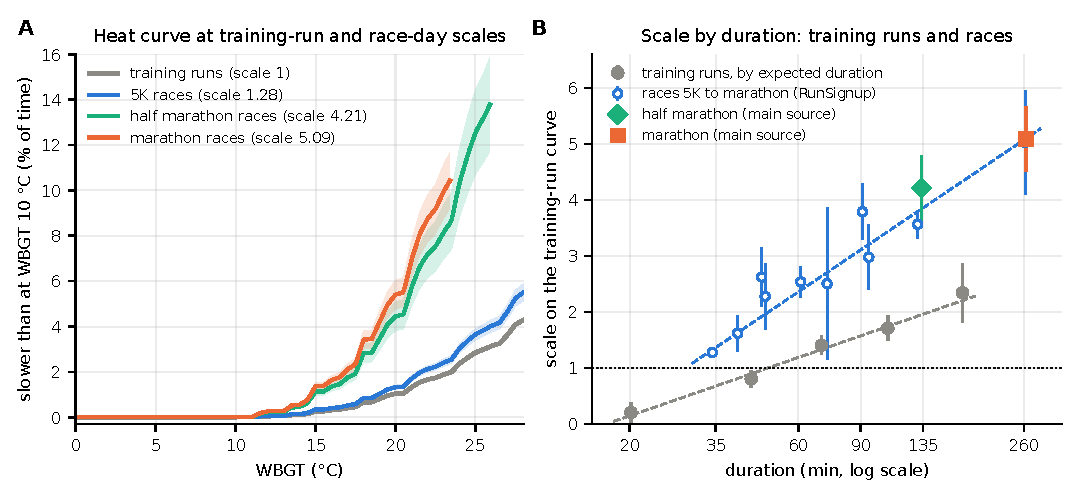
\includegraphics[width=\linewidth]{fig1_dose_response.pdf}
\caption{Training-run dose--response and race-day scale. \textbf{A}, the training-run heat curve \cW, the median runner's pace relative to WBGT 10\degC{} in counterfactual WBGT sweeps of the trained transformer (grey; zero at and below 10\degC), and the same curve multiplied by the race-day scales estimated from official results for the 5K (blue), the half marathon (green) and the marathon (orange); shaded bands are 95\% CI of the scale, and half-marathon and marathon curves are drawn up to the hottest edition in each set. \textbf{B}, within-runner scale on \cW{} for training runs in five bands of expected duration (grey; points at the band median; 95\% CI clustered by runner and by date and country; \nLtThirty, \nThirtySixty, \nSixtyNinety, \nNinetyOneFifty{} and \nGtOneFifty{} runs), race-day scales of ten distances from 5\,km to the marathon in the short-race source (open blue; course-clustered 95\% CI), and the half-marathon and marathon scales from the main official-results source (filled), placed at the median edition finish time. Dashed lines: fits on log duration across the training bands and across the ten race distances; dotted line: scale 1.}
\label{fig:dose}
\end{figure}

\begin{figure}[p]
\centering
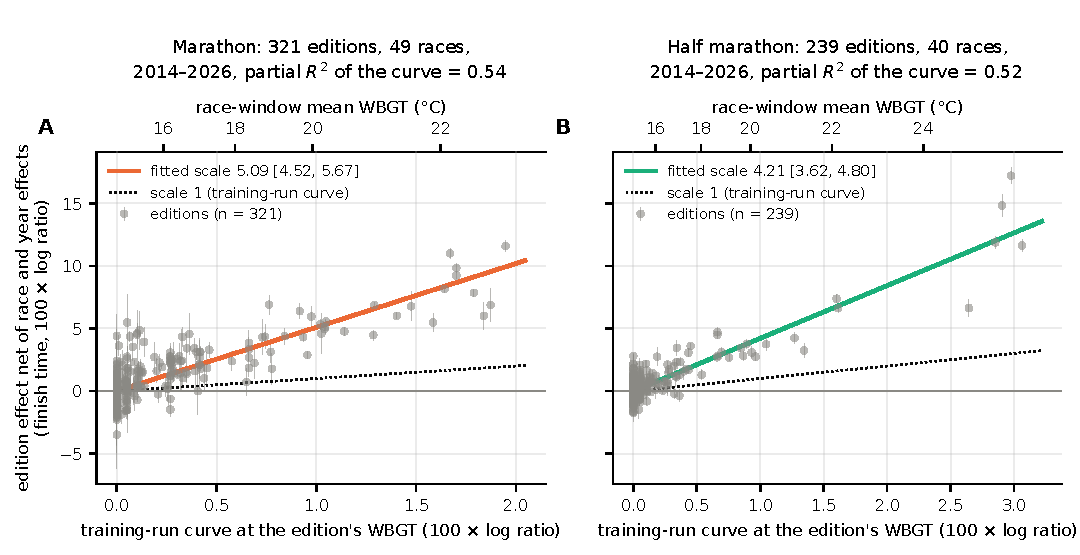
\includegraphics[width=\linewidth]{fig2_raceday_scale.pdf}
\caption{Within-person edition effects against the training-run curve at each edition's race-window WBGT. \textbf{A}, marathon, \nEdMar{} editions of \nRacesMar{} races; \textbf{B}, half marathon, \nEdHalf{} editions of \nRacesHalf{} races; 2014 to 2026 without 2020. Each point is an edition effect net of course and calendar-year fixed effects ($100 \times$ log ratio of finish time) with a 95\% CI from person-clustered standard errors. Solid line: fitted race-day scale (weighted least squares, weights $1/\mathrm{SE}^2$); dotted line: scale 1. The top axis gives the race-window mean WBGT corresponding to each curve value. Race-window WBGT is the mean from the first mass start to that start plus the edition's median finish time, at the start line. Panel titles give the partial $R^2$ of the curve beyond the fixed effects.}
\label{fig:raceday}
\end{figure}

\begin{figure}[p]
\centering
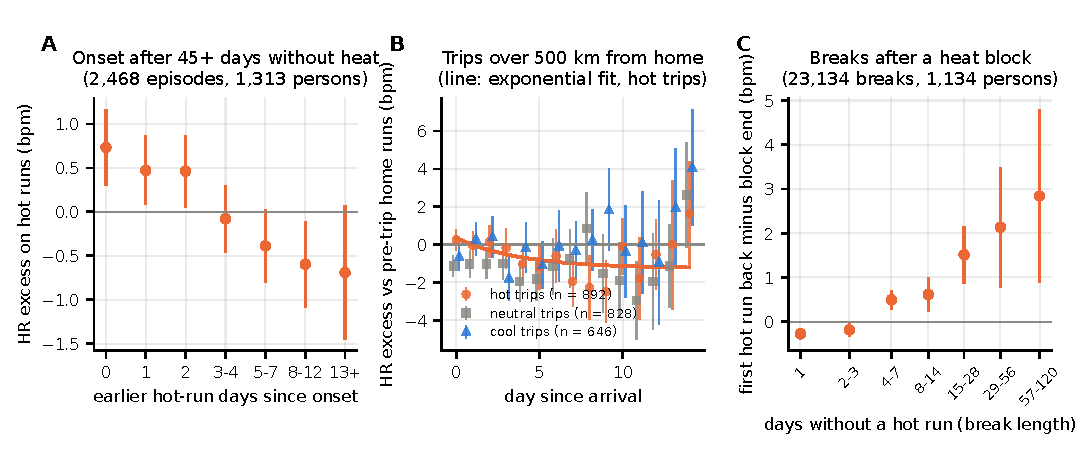
\includegraphics[width=\linewidth]{fig3_acclimation_kinetics.pdf}
\caption{Build and decay of heat acclimation in HR at matched load. The outcome is HR minus each runner's load model (pace, duration, climb), the start-hour effect and the population heat cost, relative to each design's baseline; heat is counted from WBGT 22\degC. \textbf{A}, onset: excess on hot runs by the number of earlier hot-run days after a first hot run that followed 45 or more days without one (episode fixed effects, days-since-onset trend, control for a hot run the day before; \kinOnsetEpisodes{} episodes). \textbf{B}, trips more than 500\,km from home: excess on away runs relative to home runs in the 45 days before the trip, by day since arrival, for hot ($\geq$5\degC{} warmer than home), neutral (within 2\degC) and cool ($\geq$5\degC{} cooler) trips; line, exponential fit to hot trips. \textbf{C}, breaks after a block of at least four hot-run days in 14: excess on the first hot run back minus the block's last week, by break length (\kinBreaks{} breaks). Means or coefficients with 95\% CI (person-clustered in A and C).}
\label{fig:kinetics}
\end{figure}

\begin{figure}[p]
\centering
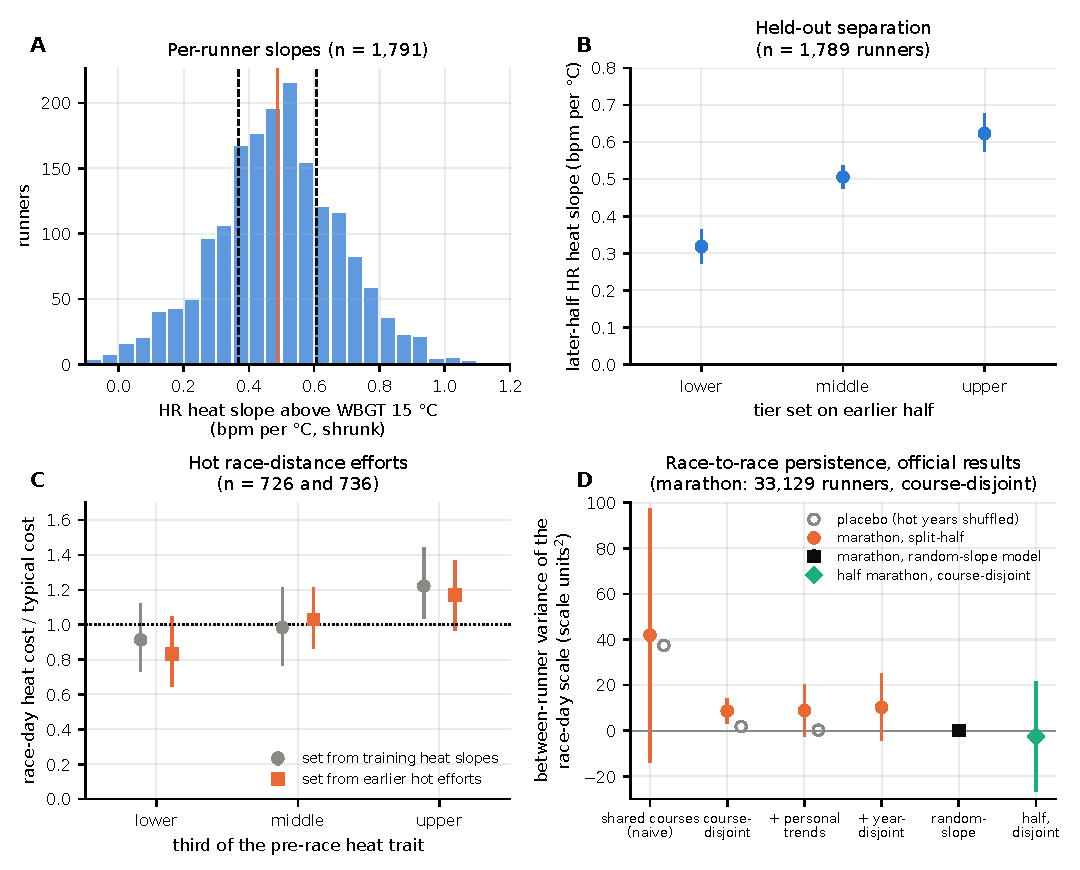
\includegraphics[width=\linewidth]{fig4_between_runner.pdf}
\caption{Between-runner differences in heat sensitivity in training and on race day. \textbf{A}, empirical-Bayes-shrunk HR heat slopes above WBGT 15\degC{} (\nSlopePersons{} runners); orange line, mean of the person slopes (\muPersons{} \bpmC); dashed lines, cut-points of three equal-probability tiers of the estimated true-slope distribution (\tierCuts{} \bpmC). \textbf{B}, later-half HR heat slope (mean and 95\% CI) by tier formed on the earlier half of each runner's history (\nTierRunners{} runners). \textbf{C}, race-day heat cost of hot race-distance efforts (WBGT 18\degC{} or above) by runners with at least one earlier hot effort, as a multiple of the population-typical cost after removing the runner's personal miss estimated from earlier data, by thirds of the training-derived heat trait (grey, \nTrainThirds{} efforts) or of the heat trait estimated from earlier race-distance efforts in the placement model (orange, \nEarlierThirds{} efforts); thirds use only data dated before each effort; 95\% CI from resampling runners; dotted line, typical cost. \textbf{D}, between-runner variance of the race-day scale in official results, estimated as the covariance of each runner's heat slopes from two halves of their races (95\% CI, delete-one-course jackknife): marathon halves sharing courses (naive), sharing no course, with personal trends, and sharing no calendar year; hollow markers, placebo with hot years shuffled within course; square, random-slope model on all repeat marathoners (upper bound shown); diamond, half marathon with halves sharing no course.}
\label{fig:between}
\end{figure}

\end{document}
" drops the line
% numbers; tables and figures already sit after the references, outside the counted span
\ifdefined\wordcountbuild
  \AtBeginDocument{\let\linenumbers\relax}
\fi

\begin{document}

% =====================================================================================================================
% TITLE PAGE
% =====================================================================================================================
\begin{titlepage}
\begin{flushleft}
{\Large\bfseries The performance cost of environmental heat in recreational distance runners: from within-runner training data to official race results\par}
\vspace{1.2em}
\textbf{Running head:} Heat cost from training to race day\par
\vspace{1.2em}
Peter Dunphy, Thomas Mulc, Gabe Cupino\par
\vspace{0.4em}
Kailo, Mountain View, CA, USA\par
\vspace{1.4em}
\textbf{Corresponding author:} \placeholder{name, postal address, e-mail address and telephone of the corresponding author}\par
\vspace{1.4em}
\textbf{Word count:} abstract \wcAbstract{} words; main text \wcMain{} words (Introduction to Conclusions, excluding the key-points box, references, tables and figure legends)\par
\textbf{Tables:} 2\quad \textbf{Figures:} 4\par
\vspace{1.4em}
\textbf{Extended version:} full methods and additional analyses are given in reference \citenum{dunphy2026extended}.\par
\vspace{1.4em}
{\small\textcolor{otred}{Working draft. Red brackets mark items to be supplied by the authors.}\par}
\end{flushleft}
\end{titlepage}

% =====================================================================================================================
% ABSTRACT
% =====================================================================================================================
\begin{onehalfspace}
\section*{Abstract}
\noindent\textbf{Purpose:} To quantify the performance cost of environmental heat in recreational runners, from training to race day, and to examine heat acclimation and between-runner differences.

\noindent\textbf{Methods:} We analysed \nRuns{} GPS-recorded training runs (\nRunners{} runners) and official results of 5-km to marathon races, computing wet-bulb globe temperature (WBGT) along each run and race window. A training-run heat curve was scaled within runner by expected duration and against within-person edition effects. Secondary outcomes were heart rate (HR) at matched load and individual differences.

\noindent\textbf{Results:} Versus 10\degC, training pace slowed at most \cFourteen\% up to WBGT 14\degC{} and \cTwentyeight\% at 28\degC; the within-runner scale rose from \scLtThirtyPt{} (runs under 30\,min) to \scGtOneFiftyPt{} (over 150\,min). Race-day scales rose with race duration, from \alphaFiveK{} (5K; 95\% CI) to \alphaHalfCI{} (half marathon) and \alphaMarCI{} (marathon), about \ratioRound{} the training scale at matched duration: \marMinTwenty{} min for a 4:00 marathon at WBGT 20\degC. In the heat, excess HR at matched load halved within \kinOnsetHalf{} hot-run days and returned with a half-life of \kinDecayHalf{} days without heat. Runners differed persistently in training HR heat slope (SD \sdPersistent{} \bpmC; at most three tiers), but this did not predict race-day heat cost, which was barely repeatable between races (reliability of a runner's race history about \persistRel).

\noindent\textbf{Conclusions:} Heat costs recreational runners more the longer the race, and about \ratioRound{} as much as training runs of equal duration.

\vspace{0.6em}
\noindent\textbf{Keywords:} wet-bulb globe temperature; heat acclimatization; marathon; half marathon; heart rate; wearable sensors
\end{onehalfspace}

\vspace{1em}
\begin{tcolorbox}[colback=white,colframe=black,boxrule=0.6pt,arc=0pt,left=6pt,right=6pt,top=4pt,bottom=4pt,title=Key points,coltitle=black,colbacktitle=gray!15,fonttitle=\bfseries]
\begin{itemize}[leftmargin=1.2em,itemsep=2pt,topsep=2pt]
\item Within the same recreational runners, the pace cost of heat on training runs was close to zero up to a WBGT of about \flatToWBGT\degC{}, accelerated above it, and grew with the duration of the run.
\item In official results, finish times followed the same curve at a scale rising with race duration, from about \alphaFiveKRound{} for the 5K to about \alphaMarRound{} for the marathon, about \ratioRound{} the cost of training runs of the same duration: \marMinTwenty{} min for a 4:00 marathon at WBGT 20\degC.
\item Heat acclimation was visible in HR at matched load, building within about \kinBuildRound{} hot runs and fading over one to two weeks without heat; runners differed persistently in their training HR response to heat (at most three groups), but neither this nor race history sorted runners reliably by race-day heat cost.
\end{itemize}
\end{tcolorbox}

\newpage
\doublespacing
\linenumbers

% =====================================================================================================================
\section{Introduction}
% =====================================================================================================================
Heat is among the most consistent environmental limits on endurance performance. During running most metabolic energy is released as heat; when the environment cannot remove it fast enough, skin blood flow competes with working muscle for cardiac output, sweat losses accumulate, and core temperature rises toward levels at which runners reduce their pace \cite{cheuvront2001,maughan2007,racinais2015}. The cost grows with the length of the event: across World Championships, sprint performances improved in the heat while endurance events were impaired by about 3\% \cite{guy2015art}. Because warming has made record heat more frequent \cite{king2017,russo2014}, more mass-participation races are run in conditions in which these limits bind.

Field estimates of the cost come mainly from race results, which show slowing that is small in cool conditions and grows with wet-bulb globe temperature (WBGT) \cite{ely2007,elhelou2012,knechtle2019,mantzios2022,vernon2021}. Most of these designs compare fields rather than people, so an edition's result also reflects who entered, started and finished; within-person designs have followed the same runners across three editions of one race \cite{tan2022}, elite athletes across races \cite{wang2024} and repeat finishers across North American marathons \cite{oliveira2026}. Controlled studies isolate the physiology and show that 5 to 14 days of heat exposure lower heart rate (HR) and core temperature at a fixed workload and improve performance in the heat \cite{periard2015,tyler2016art,tyler2024,james2017}, but they include tens of participants and rarely connect to race outcomes.

Wrist-worn GPS devices now record recreational runners' training in the conditions they actually meet, which allows within-runner comparisons of hot and cool days at scale. Large training-data studies have predicted race performance without weather \cite{smyth2020,emig2020benchmark}, and a model of wearable workouts has learned environmental effects on HR \cite{nazaret2023}, but we found no estimate of the pace cost of heat from individuals' training records and no study comparing it with race day. It is unknown whether a heat cost estimated on training runs, when a runner can slow down, shorten the session or move it to a cooler hour, describes what heat does on race day, how quickly heat exposure changes the cost in free-living runners, and whether runners differ in heat sensitivity consistently enough to be told apart.

The primary aim was to quantify the performance cost of environmental heat in recreational runners, linking a within-runner dose--response on training runs to race-day finish times in official results from 5\,km to the marathon. The secondary aims were (i) to describe how heat acclimation builds and decays in HR at matched load, and how recent exposure relates to race-day cost, and (ii) to estimate how persistent and how measurable individual differences in heat sensitivity are, in training and on race day. Against this literature the study adds four estimates: a training-run heat curve learned without a parametric form from runners' own GPS streams, whose scale is then estimated against independent official results; the ratio of race-day to training-run heat cost across ten race distances; the build and decay of acclimation from natural experiments in routine wearable records; and the persistence of individual heat sensitivity in training together with its transfer to race day. Full methods and further analyses are reported in an extended version \cite{dunphy2026extended}.

% =====================================================================================================================
\section{Methods}
% =====================================================================================================================
\subsection{Study design}
This retrospective observational study had three components: within-runner analyses of GPS-recorded training runs, analyses of race-distance efforts by the same runners, and within-person analyses of official marathon and half-marathon results, all secondary uses of existing records (see Declarations).

\subsection{Data sources and participants}
\paragraph{Training runs.} The corpus comprised outdoor runs recorded on Garmin devices by users of a training platform who had connected their accounts and permitted research use of their data. A run was retained when its mean pace was above 2.5 and below 11.5\,min\,km$^{-1}$, its mean HR above 60 and below 210\,bpm and its run-averaged WBGT at or below 28\degC, and when every covariate used below was present. The pace and HR bounds remove sensor and GPS artefacts; the WBGT ceiling reflects sparse data above it; runs without GPS were not included. Accounts belonging to one person were merged for the between-runner analyses.

\paragraph{Race-distance efforts.} Runs of 20.9 to 21.6\,km or 41.68 to 43.45\,km, with a mean HR of at least 80\% of the runner's estimated maximum, at least 20 earlier runs with weather, and a pre-race finish-time prediction, were analysed as race-distance efforts. The prediction came from a fitness model that uses only earlier training (fastest-segment times over preceding windows) \cite{dunphy2026extended}. Race labels are not available, so these efforts include an unknown share of training runs at race distance.

\paragraph{Official results.} Finish lists of marathons and half marathons held from 2014 to 2026 were assembled from a public results service, excluding virtual and cancelled editions, 2020, editions listed only as a multi-day weekend, and editions whose date or first mass-start time could not be verified from an official page or a news report. Finishers were linked across editions on normalised name, sex and a birth-year interval, with hometown as a tie-breaker; disagreement with the service's persistent member identifier, where present, bounded the false-link rate. Races from 5\,km to 10 miles came from a second public results service (United States) that records each event's scheduled start, with finishers linked within a course in the same way.

\subsection{Environmental exposure}
Exposure was outdoor WBGT ($0.7\,T_{\mathrm{nwb}} + 0.2\,T_{\mathrm{g}} + 0.1\,T_{\mathrm{a}}$), computed with the thermofeel library \cite{brimicombe2022} from air temperature, dew point, wind speed and shortwave and direct radiation, with mean radiant temperature derived from the radiation fluxes and the solar zenith angle. For training runs, weather came from a self-hosted instance of the Open-Meteo service \cite{zippenfenig2023} (the finest model available, 15-min or hourly), sampled at the start, every 15\,min and at the finish, and each run was summarised by its time-weighted mean WBGT. For each race edition, the date came from the published schedule, the start time from official pages or news reports (first mass-start wave; scheduled start for short races), and hourly ERA5 reanalysis \cite{hersbach2020} at the start line (the race city's 0.25\textdegree{} cell for short races) was interpolated and averaged from the start to the start plus the edition's median finish time. Over this window, the rise in WBGT and the degree-hours above 22\degC{} were computed, and the deviation from recent climate was the window WBGT minus the mean over the same clock window on the 60 preceding days.

A runner's recent exposure was summarised by a heat-exposure index between 0 and 1, computed from earlier runs only and updated daily: it rises in proportion to heat-weighted running time (minutes weighted from 0 at WBGT 22\degC{} to 1 at 28\degC, divided by 60 and capped at 1 per day; gain 0.15 times this stimulus times the remaining capacity) and decays by 2.5\% per day, following published kinetics \cite{racinais2015,daanen2018art}. For finishers in the official results, the published hometown was geocoded to a 1\textdegree{} cell (at least 30 persons), and a decay-weighted (14-day half-life) home WBGT over the 60 days before each race was expressed relative to the course's 60-day pre-race value.

\subsection{Outcomes}
For training runs the outcome was $100 \times \ln(\text{mean pace})$, which approximates a percentage change. For official results it was the within-person edition effect, estimated per course from same-course repeat pairs as $\ln(t_b/t_a) = e_b - e_a + \text{age term}$, with person-clustered standard errors; editions with fewer than 30 repeat pairs were dropped, and no drift term was fitted because it is collinear with the edition contrasts (long-run change enters through calendar-year effects). HR at matched load was the run's mean HR adjusted for relative speed, 30-day pace and distance, duration, climb and start hour. For race-distance efforts the outcome was the loss, $100 \times \ln(\text{actual}/\text{predicted finish time})$, re-centred on cool efforts (WBGT below 12.5\degC) of other runners, and its ratio $\rho$ to the population-typical race-day heat cost.

\subsection{Statistical analysis}
\paragraph{Training-run heat curve.} The shape of the heat response was taken from a transformer network trained on 90\% of runners to predict pace from each runner's 30 most recent activities, each represented as 128-point streams of pace, HR, cadence, power, distance, altitude, cumulative climb and WBGT, with date, latitude and activity type \cite{dunphy2026extended}. Sweeping WBGT through the trained network with all other inputs held fixed gave each runner's predicted pace across conditions. The curve \cW{} combines the median of the runners' normalised response shapes (\curveShapeRunners{} runners) with the median sensitivity of a reference sample (\curveRefRunners{} runners); it is zero at and below WBGT 10\degC{} and held constant above 28\degC{} \cite{dunphy2026extended}. These samples include \curveShapeHoldout{} and \curveRefHoldout{} runners from the network's holdout; a curve built on fitting runners alone differs from it by at most \curveHoldoutDiff{} percentage points. The network received no constraint on shape. Every magnitude reported below was estimated by regression on \cW, so the curve enters as a fixed covariate and its scale is estimated.

\paragraph{Within-runner dose--response.} On training runs, $100 \ln(\text{pace})$ was regressed on \cW{} within runner, with a cold term $\max(0, 10 - W)$, log distance, climb per kilometre (clipped at 100\,m\,km$^{-1}$) and log 30-day pace, separately within five bands of expected duration (distance times 30-day pace: under 30, 30 to 60, 60 to 90, 90 to 150 and over 150\,min), with runner-by-band intercepts. Expected rather than actual duration was used because heat itself lengthens a run, and HR was omitted because heat raises it. Race-distance runs were removed and runners needed at least 20 runs. Standard errors were clustered by runner and by date and country. A continuous version interacted \cW{} with log expected duration. Effort was examined with a label fixed before the run (the runner's usual share of maximal HR on that weekday), in thirds within runner. To check that the design does not produce a gradient by itself, the estimator was applied to data simulated with one common scale.

\paragraph{Race-day scale.} Edition effects were regressed on course and calendar-year fixed effects and $\alpha\,c(\bar W)$, where $\bar W$ is the race-window WBGT, by weighted least squares (weights $1/\mathrm{SE}^2$), separately for each distance; marathons and half marathons were also fitted jointly with a distance interaction, short-race intervals were clustered by course, and the scales of ten distances were regressed on the log of median finish time. The coefficient $\alpha$ states how many times the training-run curve the race-day cost is; dividing it by the training scale of the matching duration band gave a race-to-training factor (delta method). Fit is reported as the partial $R^2$ of the curve beyond the fixed effects, because the overall $R^2$ includes the calendar trend absorbed by the year effects. Robustness analyses used quantiles of the within-person deviations, finish-time tiers assigned from each runner's other finishes (so that tiers are not built from the outcome), a free piecewise-linear shape compared by leave-one-race-out cross-validation, and the WBGT rise and degree-hours as added terms. Official split times gave the share of the heat cost incurred in the second part of the race.

\paragraph{Recent heat exposure.} (a) Kinetics: the HR excess was a run's HR minus a within-person load model fitted on cool runs (log pace, log duration, climb), the start-hour effect and the population heat cost, on runs of at least 20\,min; a hot run lasted at least 20\,min at WBGT 22\degC{} or above. Three natural experiments used it. Onset: the first hot-run day after 45 or more days without one, with the excess on hot runs modelled by the number of earlier hot-run days (episode fixed effects, a days-since-onset trend, a control for a hot run the day before) and compared with calendar days and ambient heat by person bootstrap. Trips: runs more than 500\,km from a rolling home, classed as hot ($\geq$5\degC{} warmer than nearby home runs), neutral (within 2\degC) or cool ($\geq$5\degC{} cooler), with the excess relative to home runs in the 45 preceding days regressed on days since arrival (trip fixed effects). Breaks: after at least four hot-run days in 14, the first hot run back was compared with the block's last week, by break length. Exponential fits gave half-lives, and a recursive state (gain proportional to remaining capacity, first-order decay) was fitted by profile likelihood with a future-dose placebo. (b) Race-distance efforts: the exposure index entered the placement model below. (c) Official results: the positive deviation from recent climate was added to the edition regression, and in the hometown design $\ln(\text{finish time})$ was regressed on person and edition fixed effects and the interaction of $c(\bar W)$ with recent home climate (percent of finish time per percentage point of curve per \textdegree C), clustered by person.

\paragraph{Between-runner differences.} Each person's HR heat slope above WBGT 15\degC{} was estimated in the matched-load model (persons with at least 10 runs above 15\degC). Because errors of consecutive runs are correlated, the true between-person variance was estimated as the covariance of slopes from disjoint halves of each history: alternate calendar weeks, early against late history (the persistent part), and odd against even heat seasons. The persistent variance explained by proxies (body mass from active energy per kilometre, a stride-based height proxy, maximal HR, fitness, volume) was cross-fitted over five folds of persons, and empirical-Bayes-shrunk slopes were cut into three, four or five equal-probability tiers on the early half of each history and evaluated on the late half. Race-day placement used a linear mixed model of the loss with two effects per runner, a personal miss against the prediction that applies at every temperature and a heat trait (a multiple of the typical cost), with the exposure index and 28-day volume in the heat term and an optional training-derived prior for the trait. It was fitted by restricted maximum likelihood on four of five runner folds, each held-out effort's runner effects coming from that runner's earlier efforts only; the correlation between the two effects was fixed at zero after inspection. Pre-specified comparisons added earlier efforts, the training-derived trait and the exposure index to a population model, judged by the mean absolute error of predicted loss on hot efforts (WBGT at or above 18\degC) with runner-bootstrap intervals. Persistence of the race-day scale in official results was estimated by splitting each runner's editions into two halves that shared no course, each with warm (WBGT 15\degC{} or above) and cool editions; within each half, edition-adjusted log finish time was regressed on the curve value relative to the course mean, and the precision-weighted covariance of the two slopes estimated the persistent between-runner variance, with delete-one-course jackknife intervals and placebos that shuffled heat within runner or across years within course.

\paragraph{Inference.} Estimates are reported with 95\% confidence intervals (CI), from cluster-robust standard errors or from bootstrap resampling of runners, persons or race dates, as detailed in the extended version \cite{dunphy2026extended}. The within-runner training scale by duration and $\alpha$ for each distance were designated primary. All other analyses are secondary, were not adjusted for multiplicity, and their intervals should be read as descriptive; $p$ values are given only for key contrasts. Analyses used Python with statsmodels, scikit-learn and JAX.

% =====================================================================================================================
\section{Results}
% =====================================================================================================================
\subsection{Cohorts}
The corpus held \nRuns{} runs by \nRunners{} runners (median \runsPerRunnerMed{} runs per runner, interquartile range \runsPerRunnerIQR) recorded from \corpusFirst{} to \corpusLast{} in \nCountries{} countries (Table~\ref{tab:cohorts}). Median run WBGT was \wbgtMed\degC{} (10th to 90th percentile \wbgtPten{} to \wbgtPninety\degC); \shareEighteen\% of runs took place at 18\degC{} or above and \shareTwentytwo\% at 22\degC{} or above. There were \nEfforts{} race-distance efforts (\nEffHalf{} half, \nEffMar{} marathon) by \nEffRunners{} runners, \nEffHot{} of them at WBGT 18\degC{} or above (\nEffHotRunners{} runners). The official results comprised \nFinishes{} finishes by \nPersons{} persons, \nRepeaters{} of whom finished twice or more, and edition effects were estimable on \nCoursesEff{} courses. After exclusions (\nNoStart{} held editions outside 2020 lacked a sourced first mass-start time), \nEdMar{} marathon editions of \nRacesMar{} races and \nEdHalf{} half-marathon editions of \nRacesHalf{} races, with \nFinAnalysis{} finishes, entered the analysis. Their race-window WBGT ranged from \wbgtRangeMar\degC{} for marathons (\edMarEighteen{} editions at 18\degC{} or above, \edMarTwentytwo{} at 22\degC{} or above) and from \wbgtRangeHalf\degC{} for half marathons (\edHalfEighteen{} and \edHalfTwentytwo). The member identifier disagreed with the linkage for \falseLink\% of the persons on whom it could be checked.

\subsection{Training-run dose--response}
The training-run curve was close to zero up to WBGT 14\degC{} (\cFourteen\%) and then rose at an increasing rate, to \cSixteen\% at 16\degC, \cTwenty\% at 20\degC, \cTwentyfour\% at 24\degC{} and \cTwentyeight\% at 28\degC, relative to 10\degC{} (Fig.~\ref{fig:dose}A). Within runner, the scale on this curve increased with expected run duration, from \scLtThirty{} for runs under 30\,min (\nLtThirty{} runs) to \scThirtySixty{} (30 to 60\,min), \scSixtyNinety{} (60 to 90\,min), \scNinetyOneFifty{} (90 to 150\,min) and \scGtOneFifty{} for runs over 150\,min (\nGtOneFifty{} runs by \nGtOneFiftyRunners{} runners) (Fig.~\ref{fig:dose}B). Across the bands the scale rose by about \trainPerDoubling{} per doubling of duration. Applied to data simulated with one common scale of \placeboTrue, the estimator returned \placeboRange{} in every band. With effort fixed before the run, hard days were not steeper than easy days (difference \effortGradient\% per \textdegree C). At WBGT 20\degC, a training run of over 150\,min was therefore \longTwenty\% slower than at 10\degC{} (Table~\ref{tab:cost}).

\subsection{Race-day scale in official results}
Within-person edition effects rose with the value of the training-run curve at each edition's WBGT (Fig.~\ref{fig:raceday}). The race-day scale was $\alpha$ = \alphaMarCI{} for the marathon (partial $R^2$ of the curve \prsqMar) and \alphaHalfCI{} for the half marathon (\prsqHalf), a difference of \alphaDiff{} ($p$ = \alphaDiffP). Relative to training runs of matching duration, the race-day cost was \ratioMar{} times larger for the marathon and \ratioHalf{} times larger for the half marathon (Fig.~\ref{fig:dose}B). At a race-window WBGT of 21\degC{} a marathon took \marPctTwentyone\% longer than at 10\degC, \marMinTwentyone{} min on a 4:00 finish. Table~\ref{tab:cost} converts the scales into finish time across distances and conditions; at WBGT 20\degC{} a 4:00 marathon was \marMinTwenty{} min slower than at 10\degC. In official results of shorter races the scale was \alphaFiveK{} for the 5K (\nEdFiveK{} editions of \nCrFiveK{} races, \nWarmFiveK{} at WBGT 18\degC{} or above), \alphaTenK{} for the 10K (\nEdTenK{}, \nCrTenK{}, \nWarmTenK) and \alphaFifteen{} for 15\,km and 10 miles pooled (\nEdFifteen{}, \nCrFifteen{}, \nWarmFifteen; \alphaFifteenNoBoiler{} without the race with the largest weight). Across ten distances from 5\,km to the marathon, $\alpha$ = \durIntercept{} + \durSlope{}\,ln(median finish time, min) (weighted $R^2$ \durRsq), about \durPerDoubling{} per doubling of race duration against \trainPerDoubling{} for training runs, so races cost \raceOverTrainRange{} times the training scale at matched duration (Fig.~\ref{fig:dose}B). In this source the marathon scale was \rsuMar{} and the half-marathon scale \rsuHalf{}; shifting every start by one hour changed the scale by \startShift\%. Within each distance, the scale was highest for mid-pack finishers and lower for the fastest and slowest.

The scale did not depend on a minority of runners who slowed markedly. Estimated on the median of each edition's within-person deviations it was \alphaMarMedian{} for the marathon and \alphaHalfMedian{} for the half marathon; on the 25th percentile, \alphaMarQtf{} and \alphaHalfQtf. Finish-time tiers assigned from each runner's other finishes showed no linear trend in the marathon (\tierMarTrend{} per hour) or half marathon (\tierHalfTrend). A free piecewise shape rose earlier than the scaled curve (\freeFourteen{} against \scaledFourteen{} log points at WBGT 14\degC, marathon) but lowered leave-one-race-out error only from \rmseScaled{} to \rmseFree{} (\rmseNoWx{} without weather).

At matched mean WBGT, each degree of rise over the race window added \riseMar\% of finish time in the marathon and \riseHalf\% in the half marathon (pooled \risePooled\%). Degree-hours above 22\degC, non-zero in \nDhMar{} marathon and \nDhHalf{} half-marathon editions, were not distinguishable from zero alongside the curve (\dhMar{} and \dhHalf\% per \textdegree C\,h). In official split times (\nSplitRunners{} runners in \nSplitEd{} editions of \nSplitCourses{} courses), \lateShare\% of the heat cost in the \nSplitWarm{} warm editions fell in the second part of the race.

\subsection{Recent heat exposure}
At matched load, HR rose by \hrSlope{} \bpmC{} above WBGT 15\degC{} plus \hrSlopeTwentyfour{} above 24\degC{} (\hrRuns{} runs, \hrPersons{} persons), and this cost was larger before acclimation (Fig.~\ref{fig:kinetics}). After 45 or more days without heat (\kinOnsetEpisodes{} episodes, \kinOnsetPersons{} persons), the excess fell by \kinOnsetDecline{} bpm, half of it within \kinOnsetHalf{} hot-run days. On hot trips (\kinTrips{} trips, \kinTripPersons{} runners) the half-life was \kinTripHalf{} days and the excess declined by \kinSlopeHot{} bpm per day over the first week, against \kinSlopeNeutral{} on neutral (\kinTripsNeutral) and \kinSlopeCool{} on cool trips (\kinTripsCool); the arrival level (about \kinArrival{} bpm above neutral trips) depends on the baseline used. The count of hot-run days described the build better than calendar days (\kinCountCal\% of bootstraps) or ambient heat (\kinCountAmb\%), neither of which added to it (\kinCalAdd{} and \kinAmbAdd{} bpm). After a block of hot running (\kinBreaks{} breaks, \kinBreakPersons{} persons), the first hot run back carried \kinBreakFour, \kinBreakEight, \kinBreakFifteen{} and \kinBreakTwentynine{} bpm more excess after 4--7, 8--14, 15--28 and 29--56 days off, a decay half-life of \kinDecayHalf{} days; state models gave \kinStateOnset{} and \kinStatePanel{} days. On \kinNonhotBreaks{} breaks with non-hot runs at both ends, the hot-run rise exceeded the non-hot rise by \kinNonhotDiD{} bpm at 15--28 days, so up to about a third of the rise was not specific to heat. Saturation was not identified, and a shift in HR at every WBGT failed the future-dose placebo.

In the placement model, each unit of the exposure index changed the race-day heat cost by \scoreRace{} times the typical cost (28-day volume \volumeRace{} per SD). In official results, each degree by which race-window WBGT exceeded the 60-day climate added \devMar\% of finish time in marathons and \devHalf\% in half marathons. A warmer recent home climate went with a smaller heat cost, by \homeMarAlone{} percent of finish time per percentage point of curve per \textdegree C in marathons (\homeFinMar{} finishes, \homePersMar{} persons, \homeEdMar{} editions) and \homeHalfAlone{} in half marathons (\homeFinHalf, \homePersHalf, \homeEdHalf); for a marathon at WBGT 22\degC, a home climate 5\degC{} warmer than the course corresponds to \homeIllusMar\% (\homeIllusMarMin{} min on 4:00).

\subsection{Between-runner differences}
The true between-person SD of the HR heat slope was \sdPersistent{} \bpmC{} between the early and late halves of each history (\nSlopePersons{} persons) and \sdSeasons{} between different heat seasons (\nSeasonsPersons{} persons), against a population slope of \hrSlope. The persistent part made up \sharePersistent\% of the systematic between-person variance, the remaining \shareSameSeason\% varying within a season, and \acrossSummers\% of the alternate-week variance persisted across summers. The split-half reliability of a slope estimated from a full history was \reliability. The proxies jointly explained \proxyShare\% of the persistent variance, and the body-mass proxy \massShare\%.

Three tiers formed on the early half of each history separated later-half slopes of \tierLate{} \bpmC{} (upper minus lower \tierGap; \nTierRunners{} runners; Fig.~\ref{fig:between}A,B). The median runner's posterior probability of belonging to the assigned tier was \postThree\% with three tiers, \postFour\% with four and \postFive\% with five.

On the \nEffHot{} hot race-distance efforts (\nEffHotRunners{} runners), the held-out mean absolute error of the population model was \cpMissPop{} percentage points of finish time. The training-derived trait did not change it (\cpTrainPrior), the runner's earlier race-distance efforts reduced it by \cpRaces{} (to \cpRacesVal), and these with the exposure index by \cpCombined{} (to \cpCombinedVal). Most of the gain came from the personal miss, which applies at every temperature; the heat-specific part alone gave \cpHeatOnly. Among runners with an earlier hot effort, thirds of the estimated trait had race-day heat costs of \groupsEarlier{} times typical (upper minus lower \gapEarlier), against \groupsTrain{} (\gapTrain) for thirds of the training-derived trait (Fig.~\ref{fig:between}C), but the median posterior probability of the most probable third was only \postOneRace{} after one earlier hot effort and \postFiveRaces{} after five or more. \shareNoEarlier\% of hot efforts had no earlier hot effort; among these, training-derived thirds differed by \gapNoEarlier. Fixing the personal-miss and trait correlation at zero left the held-out error unchanged.

In official results, race-day heat cost showed little persistence between races (Fig.~\ref{fig:between}D). With marathon races split into halves sharing no course (\persistRunners{} runners, effective sample \persistNeff), the between-runner variance of the race-day scale was \persistTau{} (one-sided $p$ = \persistP), \persistTauPlacebo{} after subtracting the placebo, an SD of \persistSD{} scale units (\persistPct\% of finish time at WBGT 21\degC). The estimate was fragile: with personal trends it was \persistTrend, with halves that also shared no calendar year \persistYear, and a random-slope model fitted to all \nRepeatMar{} repeat marathoners placed it at zero (upper bound \remlUpper). A naive split sharing courses gave \naiveTau, of which shuffling hot years within course reproduced \naiveP. A runner's whole race history measured the scale with reliability \persistRel{} (90th percentile \persistRelPninety); thirds assigned from it would be right for \persistTercile\% of runners against 33\% by chance, and one earlier hot race at WBGT 21\degC{} would move the forecast for the next by about \persistShrink{} of its excess. General form persisted (correlation of cool-race levels between halves \formCorr), the warm-minus-cool contrast did not (\contrastCorr). In half marathons persistence was not identified (\persistHalf; \persistHalfRunners{} runners). Women (\womenScale) and runners finishing under 3:00 (\subThreeScale) had lower scales.

% =====================================================================================================================
\section{Discussion}
% =====================================================================================================================
\subsection{Principal findings}
On training runs, the cost of heat was negligible up to a WBGT of about \flatToWBGT\degC{} and then accelerated, and within the same runners it grew with the duration of the run. In official results, within-person finish times followed approximately the same curve at a scale rising with race duration, from about \alphaFiveKRound{} for the 5K to about \alphaMarRound{} for the marathon, roughly \ratioRound{} the cost of training runs of the same duration. Heat acclimation was visible in HR at matched load, building over about \kinBuildRound{} hot-run days and fading with a half-life of about \kinDecayRound{} days, and recent heat exposure was associated with a smaller race-day cost. Runners differed persistently in their HR response to heat in training, but race-day heat cost showed little detectable persistence between races, and the gain from a runner's earlier races came mostly from their general standing rather than from heat.

\subsection{Comparison with previous work}
The flat-then-accelerating shape agrees with syntheses of elite racing, in which performance was stable up to about 15\degC{} WBGT and declined above it \cite{mantzios2022}, and with mass-field marathon analyses \cite{ely2007,elhelou2012,knechtle2019}; the race-day response began at a lower WBGT than the scaled training curve, consistent with optimal marathon air temperatures of about 4 to 12\degC{} \cite{elhelou2012,maughan2010,llewellyn2025}. The magnitudes are of the order reported for mass fields: in seven North American marathons the 50th finisher slowed by 3.5\% between the coolest and warmest WBGT quartile and the 300th by 7.9\% \cite{ely2007}, and surveyed finishers of the warm 2018 London Marathon reported times about 14\% slower than they had expected \cite{vernon2021}. Like other within-person designs \cite{tan2022,guo2019,oliveira2026}, the present estimates compare the same people across editions, so changes in who enters or finishes affect them less; they add weather over each edition's race window from a sourced start time, a range of distances, and a scale relative to the training curve.

The dependence on duration agrees with championship data, in which endurance events were impaired and sprints were not \cite{guy2015art}, with larger losses of slower half-marathon finishers attributed to their longer exposure \cite{hodgson2022}, and with laboratory evidence that heat decrements grow as running is prolonged \cite{periard2015self,hunter2026}; it quantifies that ordering across recreational races from 5\,km upward and within individual runners' training. Elite discipline-specific slopes are not monotone in duration \cite{mantzios2022}, so the ordering may not hold at elite intensity. Duration and intensity were not separated: within a distance, mid-pack finishers lost the most and the fastest and slowest less, so the gradient across distances is not a pure effect of time on course. Earlier studies disagree on who loses most within a distance: slower runners in designs that compare finishing places \cite{ely2007,vihma2010}, faster runners in others \cite{gasparetto2020,oliveira2026,inoue2026}. The back-loading of the race-day cost agrees with marathon pacing data in which the gap between closing and opening 5-km pace widened with temperature \cite{ely2008}, with a within-runner analysis in which the penalty fell mostly in the second half \cite{oliveira2026}, and with laboratory evidence that running speed falls once core temperature approaches about 39\degC{} part-way through a hot half marathon \cite{rodrigues2020}.

The HR kinetics resemble those of controlled acclimation. Half of the build came within about \kinBuildRound{} hot-run days, as in induction studies in which the HR reduction develops most rapidly over 4 to 5 days and is virtually complete after 7 \cite{periard2015,pandolf1998}, and it followed the number of exposures rather than elapsed time or ambient heat, as in laboratory comparisons of exposure schedules \cite{willmott2018,stevens2025}. Its size, \kinOnsetDecline{} bpm, is about a tenth of the reductions measured in standardised heat-stress tests, which impose a larger and fixed heat load. The decay half-life of about \kinDecayRound{} days is close to the 60\% loss of the HR adaptation over 14 days in a laboratory decay study \cite{flouris2014}, and its interval includes the meta-analytic loss of 2.3\% per day \cite{daanen2018art}; core-temperature and sweating adaptations decay more slowly \cite{weller2007,poirier2015}, and a residual benefit of months of natural acclimatisation \cite{malgoyre2020} would not be visible within the break windows used here. Part of the rise after a break is consistent with the higher exercise HR of short-term detraining \cite{mujika2000}. The exposure index used on race-distance efforts decays at the literature rate. The added cost of a race warmer than the preceding weeks agrees with the London Marathon differential \cite{vernon2021}, and the hometown association with the advantage of athletes from warmer countries in a desert ultramarathon \cite{ioannou2018}.

Individual variation in laboratory heat strain and acclimation is well documented \cite{mee2015,corbett2018}, but we are not aware of a peer-reviewed estimate of the persistence and reliability of an individual heat response in free-living athletes at this scale. The persistent between-runner SD of \sdPersistent{} \bpmC{} is large next to the population slope, yet body size, a source of differences in heat strain in laboratory studies \cite{marino2000,cramer2014}, explained almost none of it, consistent with the small share of heat strain that individual characteristics explain at relative intensities when evaporation is not limited \cite{havenith1998,jay2011}. Most training runs are in compensable conditions, where that mechanism is weakest, and the mass proxy is indirect, so this concerns the proxy rather than body mass. On race day, at most about \persistSpreadShare{} of the extra spread of finish times in heat was persistent, so the stable HR difference seen in training is not, in these data, a usable measure of an individual's race-day heat tolerance; we found no earlier estimate of whether an individual's race-day heat cost repeats. Group differences, such as the lower scale of women and of the fastest runners, were more robust. A smaller heat effect in women agrees with some mass-field analyses \cite{vihma2010,trubee2014} but not others \cite{knechtle2021b,wang2024}, and the lower scale of the fastest runners runs against a within-runner analysis of North American marathons \cite{oliveira2026}.

\subsection{Mechanisms}
Three features of racing plausibly make heat cost more than in training of the same duration. First, a race is run close to the highest sustainable output: in training part of the heat strain is absorbed as a higher HR at an unchanged pace, whereas at race intensity it has to be paid in pace \cite{cheuvront2001,periard2015}. Second, a race fixes the distance, date and start time, while in training a runner can shorten, slow down or move to a cooler hour, the behavioural thermoregulation that dominates self-paced exercise in heat \cite{flouris2015,junge2016}, which attenuates the training estimate. Third, race pace is set in advance and corrected late, which fits the back-loaded cost in the splits \cite{rodrigues2020}. The race-day scale therefore combines physiology with pacing and selection, and is not a purely physiological multiplier.

\subsection{Practical applications}
For a recreational marathoner, heat begins to cost time at a WBGT of about \costStartRange\degC{} and the cost rises quickly: about \marMinSixteen, \marMinEighteen, \marMinTwenty{} and \marMinTwentytwo{} min for a 4:00 runner at 16, 18, 20 and 22\degC, and less over shorter races (Table~\ref{tab:cost}). Slowing on hot training runs, even long ones, understates the race-day cost, so goals and pacing plans should follow the forecast race-window WBGT rather than training experience. The HR strain of heat eases after a few hot runs and the benefit fades over one to two weeks without heat, so hot running in the last weeks before a race, or arriving early, is what counts. Neither training data nor race history sorted individual runners reliably by race-day heat tolerance, so individual adjustments beyond the population scale are not supported by these data.

\subsection{Strengths and limitations}
Strengths are within-person designs on training and race data, which hold ability constant; race weather from each edition's official date, start and location; samples large enough to resolve the warm range; and independent sources analysed on a common heat curve. The design is observational, and the race-day scale absorbs pacing, field composition and selection; only finishers are observed, and withdrawals rise steeply with heat \cite{roberts2010}, so the scale is biased downward. The training-to-race factor divides a race-day scale from official-results finishers by a training scale from device users. Exposure comes from gridded weather fields rather than on-course measurement. Marathon editions reached a race-window WBGT of \wbgtMaxMar\degC, with \edMarTwentytwo{} at 22\degC{} or above, so costs beyond about 22\degC{} are extrapolations. The corpus consists of self-selected device users, and its race-distance efforts are not confirmed races. The curve comes from a learned model and $\alpha$ is a ratio to it, and a single scale only approximates the race-day shape. Short-race results are from the United States only, with weather at the race city. Linkage relies on names, HR was measured optically, sex was not observed in the corpus, secondary analyses were not adjusted for multiplicity, and one placement-model choice was made after inspection.

% =====================================================================================================================
\section{Conclusions}
% =====================================================================================================================
Environmental heat slows recreational distance runners little below a WBGT of about \flatToWBGT\degC{} and progressively more above it. The same curve, estimated within runners on training runs, describes race-day finish times in official results at a scale that rises with race duration, from about \alphaFiveKRound{} for the 5K to about \alphaMarRound{} for the marathon, roughly \ratioRound{} the cost of training runs of the same duration. Recent heat exposure reduces the HR cost of running in the heat within a few hot runs, a benefit that fades with a half-life of about \kinDecayRound{} days, and is associated with a smaller race-day cost. Runners differ persistently in their HR response to heat in training, but race-day heat cost is barely repeatable between races, so neither training data nor race history sorts individual runners reliably by race-day heat tolerance. What is new relative to earlier work is a heat curve learned from individuals' training records and tested on official results, the ratio of race-day to training cost across race distances, acclimation kinetics from routine wearable data, and a direct test showing that individual heat sensitivity measured in training does not carry to race day.

% =====================================================================================================================
\section*{Declarations}
% =====================================================================================================================
\paragraph{Ethics approval.} \placeholder{Ethics statement to be completed by the authors: name of the reviewing body and reference number, or the basis for exemption.} This study is a secondary analysis of de-identified training records held by a training platform and of finish lists publicly posted by race organisers and timing services. No individual is identifiable in any reported result.

\paragraph{Consent to participate.} \placeholder{Confirm the wording of the platform's research-use consent.} Platform users permitted research use of their data. Finishers in public results did not consent individually; only aggregate estimates are reported, and no names or individual results are reproduced.

\paragraph{Funding.} \placeholder{Funding statement.}

\paragraph{Competing interests.} \placeholder{Competing-interests statement to be completed.} All authors are affiliated with Kailo, the company whose training platform supplied the training-run data.

\paragraph{Data and code availability.} The training-run data contain location traces and cannot be shared publicly; \placeholder{access conditions}. Official results are publicly posted by race organisers; the person-linked tables derived from them are not shared because they are built from names. Analysis code and aggregate tables are available at \placeholder{repository}.

\paragraph{Author contributions (CRediT).} \placeholder{Conceptualization; Data curation; Formal analysis; Methodology; Software; Visualization; Writing, original draft; Writing, review and editing: to be assigned.}

\paragraph{Acknowledgements.} \placeholder{Acknowledgements.}

% =====================================================================================================================
\clearpage
\nolinenumbers
\singlespacing
\bibliographystyle{vancouver}
\bibliography{../references,../tommy_refs,journal_refs}

% =====================================================================================================================
% TABLES
% =====================================================================================================================
\clearpage
\begin{table}[p]
\centering
\caption{Characteristics of the three data sets. Values are counts or median (interquartile range) unless stated.}
\label{tab:cohorts}
\small
\renewcommand{\arraystretch}{1.25}
\begin{tabular}{@{}>{\raggedright\arraybackslash}p{2.9cm}>{\raggedright\arraybackslash}p{4.1cm}>{\raggedright\arraybackslash}p{3.6cm}>{\raggedright\arraybackslash}p{4.6cm}@{}}
\toprule
 & Training runs & Race-distance efforts & Official results \\
\midrule
Source & GPS wrist devices, users of a training platform & Subset of the training-run corpus & Public results service, marathons and half marathons \\
Period & \corpusFirst{} to \corpusLast & \corpusFirst{} to \effortsLast & 2014 to 2026 (2020 excluded) \\
Units & \nRuns{} runs by \nRunners{} runners; runs per runner \runsPerRunnerMed{} (\runsPerRunnerIQR) & \nEfforts{} efforts (\nEffHalf{} half, \nEffMar{} marathon) by \nEffRunners{} runners & \nFinishes{} finishes by \nPersons{} persons, \nRepeaters{} with two or more \\
Analysed subset & All runs; between-runner analyses: \nSlopePersons{} persons with 10 or more runs above 15\degC & WBGT 18\degC{} or above: \nEffHot{} efforts by \nEffHotRunners{} runners & Marathon: \nEdMar{} editions of \nRacesMar{} races, \finMar{} finishes; half marathon: \nEdHalf{} editions of \nRacesHalf{} races, \finHalf{} finishes \\
Distance, duration & \medDist{} km; \medDur{} min & 20.9--21.6 or 41.68--43.45\,km & Median edition finish time: marathon \medFinMar, half \medFinHalf{} (h:min) \\
Pace, heart rate & \medPace{} min\,km$^{-1}$; \medHR{} bpm & Mean HR 80\% of maximum or more & Not recorded \\
Exposure (WBGT) & Run mean \wbgtMed\degC{} (10th--90th percentile \wbgtPten--\wbgtPninety); \shareEighteen\% of runs at 18\degC{} or above, \shareTwentytwo\% at 22\degC{} or above & Run mean, as for training runs & Race-window mean: marathon \wbgtRangeMar\degC{} (\edMarEighteen{} editions at 18\degC{} or above, \edMarTwentytwo{} at 22\degC{} or above); half \wbgtRangeHalf\degC{} (\edHalfEighteen, \edHalfTwentytwo) \\
Weather source & Finest available model field, sampled every 15\,min along the run & As for training runs & ERA5 at the start line, first mass start to median finish \\
Outcome & $100\ln(\text{pace})$; HR at matched load & Loss against a pre-race prediction & Within-person edition effect \\
\bottomrule
\end{tabular}
\par\smallskip
\parbox{\linewidth}{\footnotesize Countries of training runs: \nCountries{} (United States \shareUS\%, South Korea \shareKR\%, United Kingdom \shareGB\%).}
\end{table}

\begin{table}[p]
\centering
\caption{Heat cost relative to WBGT 10\degC{} implied by the estimated scales: percent of time, with minutes on a reference finish time in parentheses (5K 0:30, 10K 1:00, 15\,km and 10 miles 1:30, half marathon 2:00, marathon 4:00).}
\label{tab:cost}
\small
\renewcommand{\arraystretch}{1.35}
\setlength{\tabcolsep}{5pt}
\begin{tabular}{@{}lccccc@{}}
\toprule
 & & \multicolumn{4}{c}{Race-window or run WBGT (\textdegree C)} \\
\cmidrule(lr){3-6}
 & Scale [95\% CI] & 16 & 18 & 20 & 22 \\
\midrule
Training runs, all & \TabTr \\
Training runs over 150\,min & \TabLong \\
5K & \TabFiveK \\
10K & \TabTenK \\
15\,km and 10 miles & \TabFifteen \\
Half marathon & \TabHalf \\
Marathon & \TabMar \\
\bottomrule
\end{tabular}
\par\smallskip
\parbox{\linewidth}{\footnotesize Scales multiply the training-run curve \cW; training runs over 150\,min use the within-runner scale of that expected-duration band; 5K to 10 miles use course-clustered intervals; half marathon and marathon use the main official-results source. Percentages are $100\,[\exp(s\,c_{\log}(W)/100) - 1]$ for scale $s$ and the curve in log points $c_{\log}$. Only \edMarTwentytwo{} marathon and \edHalfTwentytwo{} half-marathon editions had a race-window WBGT of 22\degC{} or above.}
\end{table}

% =====================================================================================================================
% FIGURES (legends and figures)
% =====================================================================================================================
\clearpage
\begin{figure}[p]
\centering
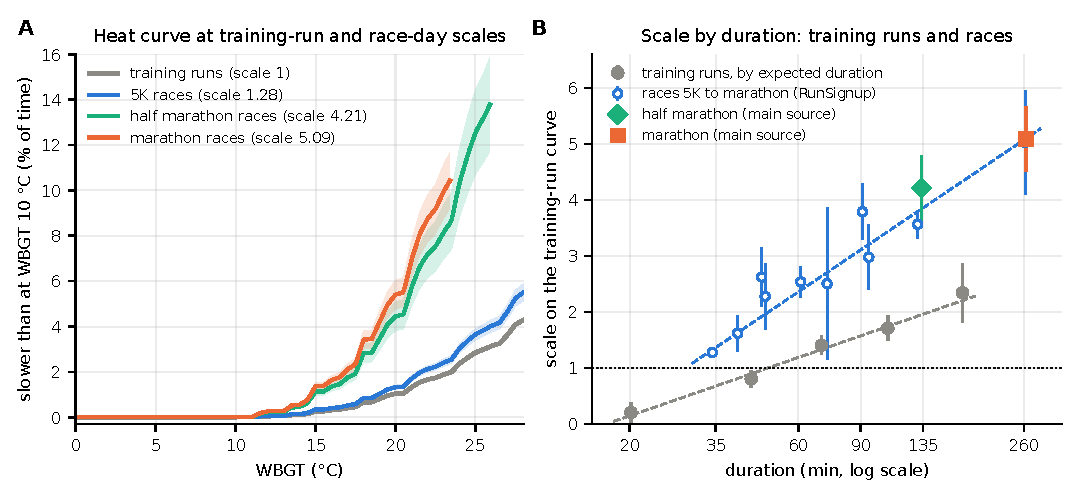
\includegraphics[width=\linewidth]{fig1_dose_response.pdf}
\caption{Training-run dose--response and race-day scale. \textbf{A}, the training-run heat curve \cW, the median runner's pace relative to WBGT 10\degC{} in counterfactual WBGT sweeps of the trained transformer (grey; zero at and below 10\degC), and the same curve multiplied by the race-day scales estimated from official results for the 5K (blue), the half marathon (green) and the marathon (orange); shaded bands are 95\% CI of the scale, and half-marathon and marathon curves are drawn up to the hottest edition in each set. \textbf{B}, within-runner scale on \cW{} for training runs in five bands of expected duration (grey; points at the band median; 95\% CI clustered by runner and by date and country; \nLtThirty, \nThirtySixty, \nSixtyNinety, \nNinetyOneFifty{} and \nGtOneFifty{} runs), race-day scales of ten distances from 5\,km to the marathon in the short-race source (open blue; course-clustered 95\% CI), and the half-marathon and marathon scales from the main official-results source (filled), placed at the median edition finish time. Dashed lines: fits on log duration across the training bands and across the ten race distances; dotted line: scale 1.}
\label{fig:dose}
\end{figure}

\begin{figure}[p]
\centering
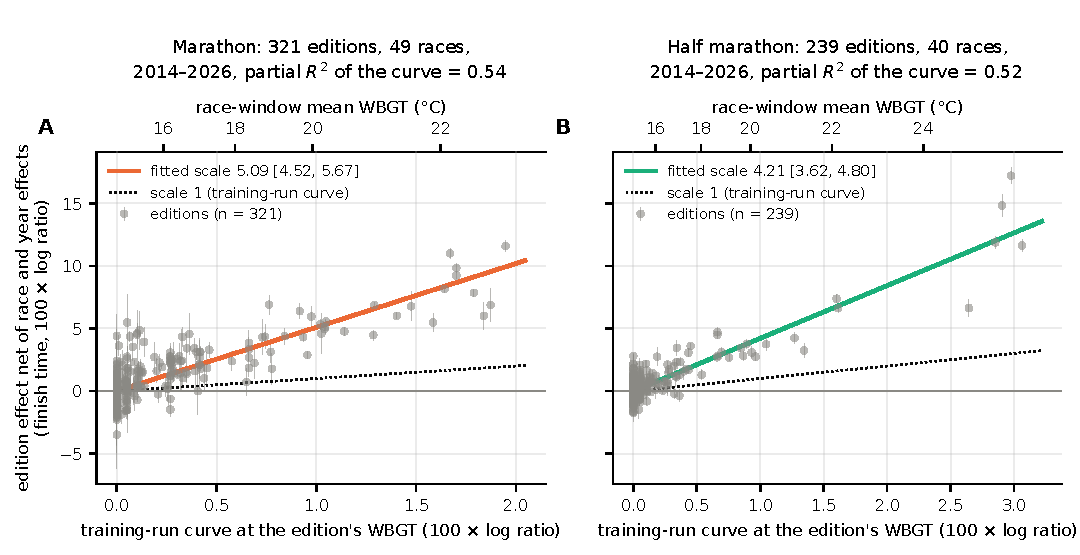
\includegraphics[width=\linewidth]{fig2_raceday_scale.pdf}
\caption{Within-person edition effects against the training-run curve at each edition's race-window WBGT. \textbf{A}, marathon, \nEdMar{} editions of \nRacesMar{} races; \textbf{B}, half marathon, \nEdHalf{} editions of \nRacesHalf{} races; 2014 to 2026 without 2020. Each point is an edition effect net of course and calendar-year fixed effects ($100 \times$ log ratio of finish time) with a 95\% CI from person-clustered standard errors. Solid line: fitted race-day scale (weighted least squares, weights $1/\mathrm{SE}^2$); dotted line: scale 1. The top axis gives the race-window mean WBGT corresponding to each curve value. Race-window WBGT is the mean from the first mass start to that start plus the edition's median finish time, at the start line. Panel titles give the partial $R^2$ of the curve beyond the fixed effects.}
\label{fig:raceday}
\end{figure}

\begin{figure}[p]
\centering
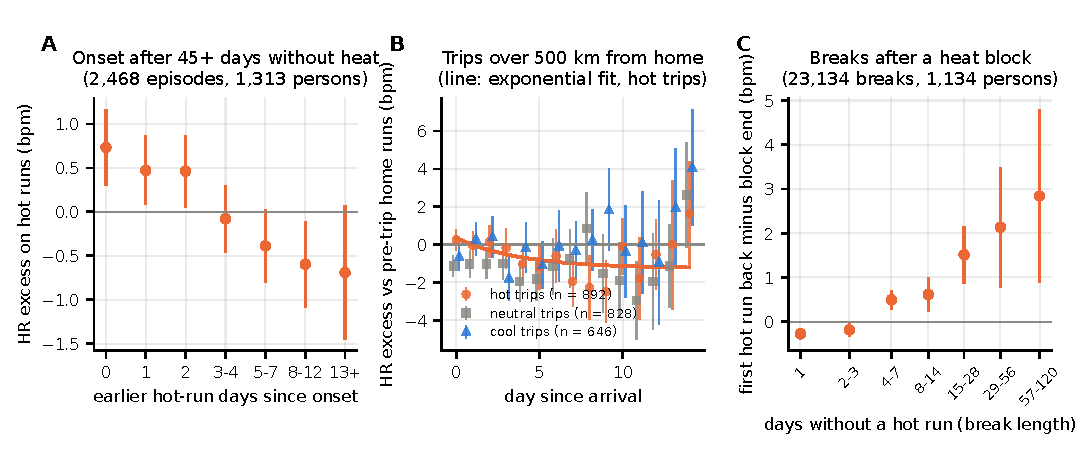
\includegraphics[width=\linewidth]{fig3_acclimation_kinetics.pdf}
\caption{Build and decay of heat acclimation in HR at matched load. The outcome is HR minus each runner's load model (pace, duration, climb), the start-hour effect and the population heat cost, relative to each design's baseline; heat is counted from WBGT 22\degC. \textbf{A}, onset: excess on hot runs by the number of earlier hot-run days after a first hot run that followed 45 or more days without one (episode fixed effects, days-since-onset trend, control for a hot run the day before; \kinOnsetEpisodes{} episodes). \textbf{B}, trips more than 500\,km from home: excess on away runs relative to home runs in the 45 days before the trip, by day since arrival, for hot ($\geq$5\degC{} warmer than home), neutral (within 2\degC) and cool ($\geq$5\degC{} cooler) trips; line, exponential fit to hot trips. \textbf{C}, breaks after a block of at least four hot-run days in 14: excess on the first hot run back minus the block's last week, by break length (\kinBreaks{} breaks). Means or coefficients with 95\% CI (person-clustered in A and C).}
\label{fig:kinetics}
\end{figure}

\begin{figure}[p]
\centering
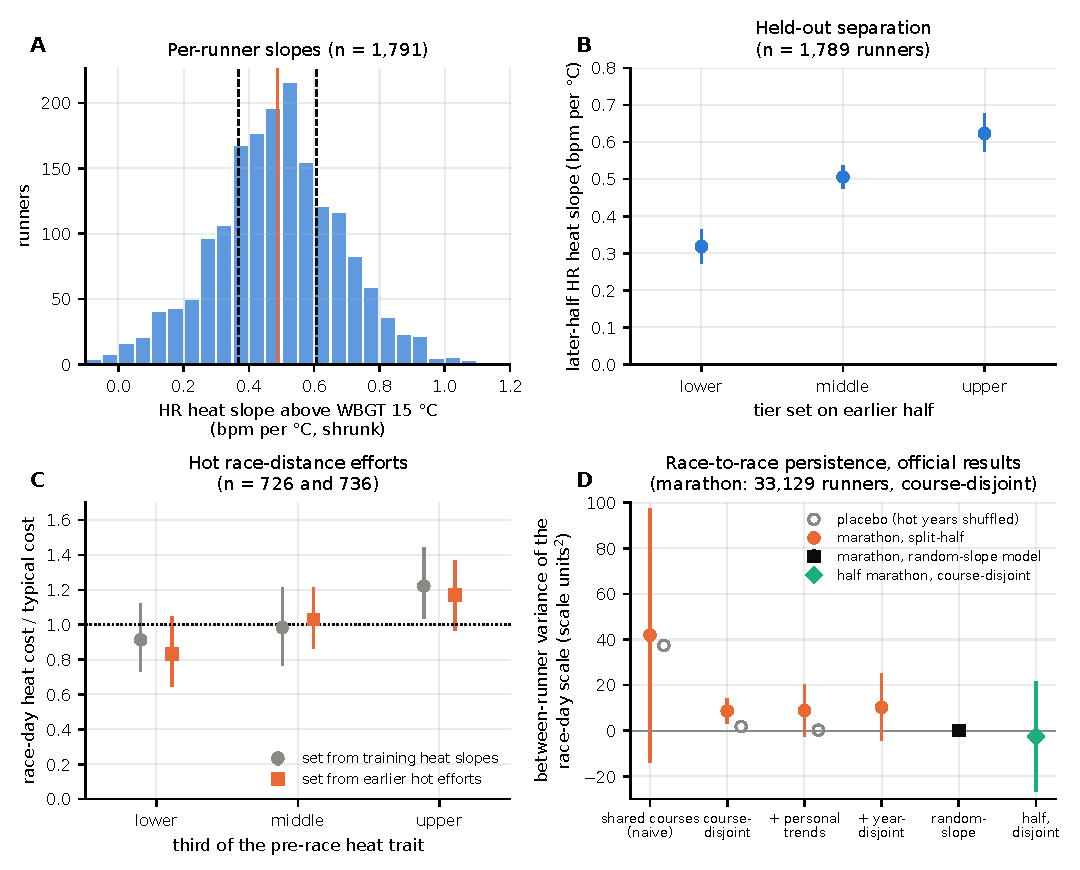
\includegraphics[width=\linewidth]{fig4_between_runner.pdf}
\caption{Between-runner differences in heat sensitivity in training and on race day. \textbf{A}, empirical-Bayes-shrunk HR heat slopes above WBGT 15\degC{} (\nSlopePersons{} runners); orange line, mean of the person slopes (\muPersons{} \bpmC); dashed lines, cut-points of three equal-probability tiers of the estimated true-slope distribution (\tierCuts{} \bpmC). \textbf{B}, later-half HR heat slope (mean and 95\% CI) by tier formed on the earlier half of each runner's history (\nTierRunners{} runners). \textbf{C}, race-day heat cost of hot race-distance efforts (WBGT 18\degC{} or above) by runners with at least one earlier hot effort, as a multiple of the population-typical cost after removing the runner's personal miss estimated from earlier data, by thirds of the training-derived heat trait (grey, \nTrainThirds{} efforts) or of the heat trait estimated from earlier race-distance efforts in the placement model (orange, \nEarlierThirds{} efforts); thirds use only data dated before each effort; 95\% CI from resampling runners; dotted line, typical cost. \textbf{D}, between-runner variance of the race-day scale in official results, estimated as the covariance of each runner's heat slopes from two halves of their races (95\% CI, delete-one-course jackknife): marathon halves sharing courses (naive), sharing no course, with personal trends, and sharing no calendar year; hollow markers, placebo with hot years shuffled within course; square, random-slope model on all repeat marathoners (upper bound shown); diamond, half marathon with halves sharing no course.}
\label{fig:between}
\end{figure}

\end{document}
" drops the line
% numbers; tables and figures already sit after the references, outside the counted span
\ifdefined\wordcountbuild
  \AtBeginDocument{\let\linenumbers\relax}
\fi

\begin{document}

% =====================================================================================================================
% TITLE PAGE
% =====================================================================================================================
\begin{titlepage}
\begin{flushleft}
{\Large\bfseries The performance cost of environmental heat in recreational distance runners: from within-runner training data to official race results\par}
\vspace{1.2em}
\textbf{Running head:} Heat cost from training to race day\par
\vspace{1.2em}
Peter Dunphy, Thomas Mulc, Gabe Cupino\par
\vspace{0.4em}
Kailo, Mountain View, CA, USA\par
\vspace{1.4em}
\textbf{Corresponding author:} \placeholder{name, postal address, e-mail address and telephone of the corresponding author}\par
\vspace{1.4em}
\textbf{Word count:} abstract \wcAbstract{} words; main text \wcMain{} words (Introduction to Conclusions, excluding the key-points box, references, tables and figure legends)\par
\textbf{Tables:} 2\quad \textbf{Figures:} 4\par
\vspace{1.4em}
\textbf{Extended version:} full methods and additional analyses are given in reference \citenum{dunphy2026extended}.\par
\vspace{1.4em}
{\small\textcolor{otred}{Working draft. Red brackets mark items to be supplied by the authors.}\par}
\end{flushleft}
\end{titlepage}

% =====================================================================================================================
% ABSTRACT
% =====================================================================================================================
\begin{onehalfspace}
\section*{Abstract}
\noindent\textbf{Purpose:} To quantify the performance cost of environmental heat in recreational runners, from training to race day, and to examine heat acclimation and between-runner differences.

\noindent\textbf{Methods:} We analysed \nRuns{} GPS-recorded training runs (\nRunners{} runners) and official results of 5-km to marathon races, computing wet-bulb globe temperature (WBGT) along each run and race window. A training-run heat curve was scaled within runner by expected duration and against within-person edition effects. Secondary outcomes were heart rate (HR) at matched load and individual differences.

\noindent\textbf{Results:} Versus 10\degC, training pace slowed at most \cFourteen\% up to WBGT 14\degC{} and \cTwentyeight\% at 28\degC; the within-runner scale rose from \scLtThirtyPt{} (runs under 30\,min) to \scGtOneFiftyPt{} (over 150\,min). Race-day scales rose with race duration, from \alphaFiveK{} (5K; 95\% CI) to \alphaHalfCI{} (half marathon) and \alphaMarCI{} (marathon), about \ratioRound{} the training scale at matched duration: \marMinTwenty{} min for a 4:00 marathon at WBGT 20\degC. In the heat, excess HR at matched load halved within \kinOnsetHalf{} hot-run days and returned with a half-life of \kinDecayHalf{} days without heat. Runners differed persistently in training HR heat slope (SD \sdPersistent{} \bpmC; at most three tiers), but this did not predict race-day heat cost, which was barely repeatable between races (reliability of a runner's race history about \persistRel).

\noindent\textbf{Conclusions:} Heat costs recreational runners more the longer the race, and about \ratioRound{} as much as training runs of equal duration.

\vspace{0.6em}
\noindent\textbf{Keywords:} wet-bulb globe temperature; heat acclimatization; marathon; half marathon; heart rate; wearable sensors
\end{onehalfspace}

\vspace{1em}
\begin{tcolorbox}[colback=white,colframe=black,boxrule=0.6pt,arc=0pt,left=6pt,right=6pt,top=4pt,bottom=4pt,title=Key points,coltitle=black,colbacktitle=gray!15,fonttitle=\bfseries]
\begin{itemize}[leftmargin=1.2em,itemsep=2pt,topsep=2pt]
\item Within the same recreational runners, the pace cost of heat on training runs was close to zero up to a WBGT of about \flatToWBGT\degC{}, accelerated above it, and grew with the duration of the run.
\item In official results, finish times followed the same curve at a scale rising with race duration, from about \alphaFiveKRound{} for the 5K to about \alphaMarRound{} for the marathon, about \ratioRound{} the cost of training runs of the same duration: \marMinTwenty{} min for a 4:00 marathon at WBGT 20\degC.
\item Heat acclimation was visible in HR at matched load, building within about \kinBuildRound{} hot runs and fading over one to two weeks without heat; runners differed persistently in their training HR response to heat (at most three groups), but neither this nor race history sorted runners reliably by race-day heat cost.
\end{itemize}
\end{tcolorbox}

\newpage
\doublespacing
\linenumbers

% =====================================================================================================================
\section{Introduction}
% =====================================================================================================================
Heat is among the most consistent environmental limits on endurance performance. During running most metabolic energy is released as heat; when the environment cannot remove it fast enough, skin blood flow competes with working muscle for cardiac output, sweat losses accumulate, and core temperature rises toward levels at which runners reduce their pace \cite{cheuvront2001,maughan2007,racinais2015}. The cost grows with the length of the event: across World Championships, sprint performances improved in the heat while endurance events were impaired by about 3\% \cite{guy2015art}. Because warming has made record heat more frequent \cite{king2017,russo2014}, more mass-participation races are run in conditions in which these limits bind.

Field estimates of the cost come mainly from race results, which show slowing that is small in cool conditions and grows with wet-bulb globe temperature (WBGT) \cite{ely2007,elhelou2012,knechtle2019,mantzios2022,vernon2021}. Most of these designs compare fields rather than people, so an edition's result also reflects who entered, started and finished; within-person designs have followed the same runners across three editions of one race \cite{tan2022}, elite athletes across races \cite{wang2024} and repeat finishers across North American marathons \cite{oliveira2026}. Controlled studies isolate the physiology and show that 5 to 14 days of heat exposure lower heart rate (HR) and core temperature at a fixed workload and improve performance in the heat \cite{periard2015,tyler2016art,tyler2024,james2017}, but they include tens of participants and rarely connect to race outcomes.

Wrist-worn GPS devices now record recreational runners' training in the conditions they actually meet, which allows within-runner comparisons of hot and cool days at scale. Large training-data studies have predicted race performance without weather \cite{smyth2020,emig2020benchmark}, and a model of wearable workouts has learned environmental effects on HR \cite{nazaret2023}, but we found no estimate of the pace cost of heat from individuals' training records and no study comparing it with race day. It is unknown whether a heat cost estimated on training runs, when a runner can slow down, shorten the session or move it to a cooler hour, describes what heat does on race day, how quickly heat exposure changes the cost in free-living runners, and whether runners differ in heat sensitivity consistently enough to be told apart.

The primary aim was to quantify the performance cost of environmental heat in recreational runners, linking a within-runner dose--response on training runs to race-day finish times in official results from 5\,km to the marathon. The secondary aims were (i) to describe how heat acclimation builds and decays in HR at matched load, and how recent exposure relates to race-day cost, and (ii) to estimate how persistent and how measurable individual differences in heat sensitivity are, in training and on race day. Against this literature the study adds four estimates: a training-run heat curve learned without a parametric form from runners' own GPS streams, whose scale is then estimated against independent official results; the ratio of race-day to training-run heat cost across ten race distances; the build and decay of acclimation from natural experiments in routine wearable records; and the persistence of individual heat sensitivity in training together with its transfer to race day. Full methods and further analyses are reported in an extended version \cite{dunphy2026extended}.

% =====================================================================================================================
\section{Methods}
% =====================================================================================================================
\subsection{Study design}
This retrospective observational study had three components: within-runner analyses of GPS-recorded training runs, analyses of race-distance efforts by the same runners, and within-person analyses of official marathon and half-marathon results, all secondary uses of existing records (see Declarations).

\subsection{Data sources and participants}
\paragraph{Training runs.} The corpus comprised outdoor runs recorded on Garmin devices by users of a training platform who had connected their accounts and permitted research use of their data. A run was retained when its mean pace was above 2.5 and below 11.5\,min\,km$^{-1}$, its mean HR above 60 and below 210\,bpm and its run-averaged WBGT at or below 28\degC, and when every covariate used below was present. The pace and HR bounds remove sensor and GPS artefacts; the WBGT ceiling reflects sparse data above it; runs without GPS were not included. Accounts belonging to one person were merged for the between-runner analyses.

\paragraph{Race-distance efforts.} Runs of 20.9 to 21.6\,km or 41.68 to 43.45\,km, with a mean HR of at least 80\% of the runner's estimated maximum, at least 20 earlier runs with weather, and a pre-race finish-time prediction, were analysed as race-distance efforts. The prediction came from a fitness model that uses only earlier training (fastest-segment times over preceding windows) \cite{dunphy2026extended}. Race labels are not available, so these efforts include an unknown share of training runs at race distance.

\paragraph{Official results.} Finish lists of marathons and half marathons held from 2014 to 2026 were assembled from a public results service, excluding virtual and cancelled editions, 2020, editions listed only as a multi-day weekend, and editions whose date or first mass-start time could not be verified from an official page or a news report. Finishers were linked across editions on normalised name, sex and a birth-year interval, with hometown as a tie-breaker; disagreement with the service's persistent member identifier, where present, bounded the false-link rate. Races from 5\,km to 10 miles came from a second public results service (United States) that records each event's scheduled start, with finishers linked within a course in the same way.

\subsection{Environmental exposure}
Exposure was outdoor WBGT ($0.7\,T_{\mathrm{nwb}} + 0.2\,T_{\mathrm{g}} + 0.1\,T_{\mathrm{a}}$), computed with the thermofeel library \cite{brimicombe2022} from air temperature, dew point, wind speed and shortwave and direct radiation, with mean radiant temperature derived from the radiation fluxes and the solar zenith angle. For training runs, weather came from a self-hosted instance of the Open-Meteo service \cite{zippenfenig2023} (the finest model available, 15-min or hourly), sampled at the start, every 15\,min and at the finish, and each run was summarised by its time-weighted mean WBGT. For each race edition, the date came from the published schedule, the start time from official pages or news reports (first mass-start wave; scheduled start for short races), and hourly ERA5 reanalysis \cite{hersbach2020} at the start line (the race city's 0.25\textdegree{} cell for short races) was interpolated and averaged from the start to the start plus the edition's median finish time. Over this window, the rise in WBGT and the degree-hours above 22\degC{} were computed, and the deviation from recent climate was the window WBGT minus the mean over the same clock window on the 60 preceding days.

A runner's recent exposure was summarised by a heat-exposure index between 0 and 1, computed from earlier runs only and updated daily: it rises in proportion to heat-weighted running time (minutes weighted from 0 at WBGT 22\degC{} to 1 at 28\degC, divided by 60 and capped at 1 per day; gain 0.15 times this stimulus times the remaining capacity) and decays by 2.5\% per day, following published kinetics \cite{racinais2015,daanen2018art}. For finishers in the official results, the published hometown was geocoded to a 1\textdegree{} cell (at least 30 persons), and a decay-weighted (14-day half-life) home WBGT over the 60 days before each race was expressed relative to the course's 60-day pre-race value.

\subsection{Outcomes}
For training runs the outcome was $100 \times \ln(\text{mean pace})$, which approximates a percentage change. For official results it was the within-person edition effect, estimated per course from same-course repeat pairs as $\ln(t_b/t_a) = e_b - e_a + \text{age term}$, with person-clustered standard errors; editions with fewer than 30 repeat pairs were dropped, and no drift term was fitted because it is collinear with the edition contrasts (long-run change enters through calendar-year effects). HR at matched load was the run's mean HR adjusted for relative speed, 30-day pace and distance, duration, climb and start hour. For race-distance efforts the outcome was the loss, $100 \times \ln(\text{actual}/\text{predicted finish time})$, re-centred on cool efforts (WBGT below 12.5\degC) of other runners, and its ratio $\rho$ to the population-typical race-day heat cost.

\subsection{Statistical analysis}
\paragraph{Training-run heat curve.} The shape of the heat response was taken from a transformer network trained on 90\% of runners to predict pace from each runner's 30 most recent activities, each represented as 128-point streams of pace, HR, cadence, power, distance, altitude, cumulative climb and WBGT, with date, latitude and activity type \cite{dunphy2026extended}. Sweeping WBGT through the trained network with all other inputs held fixed gave each runner's predicted pace across conditions. The curve \cW{} combines the median of the runners' normalised response shapes (\curveShapeRunners{} runners) with the median sensitivity of a reference sample (\curveRefRunners{} runners); it is zero at and below WBGT 10\degC{} and held constant above 28\degC{} \cite{dunphy2026extended}. These samples include \curveShapeHoldout{} and \curveRefHoldout{} runners from the network's holdout; a curve built on fitting runners alone differs from it by at most \curveHoldoutDiff{} percentage points. The network received no constraint on shape. Every magnitude reported below was estimated by regression on \cW, so the curve enters as a fixed covariate and its scale is estimated.

\paragraph{Within-runner dose--response.} On training runs, $100 \ln(\text{pace})$ was regressed on \cW{} within runner, with a cold term $\max(0, 10 - W)$, log distance, climb per kilometre (clipped at 100\,m\,km$^{-1}$) and log 30-day pace, separately within five bands of expected duration (distance times 30-day pace: under 30, 30 to 60, 60 to 90, 90 to 150 and over 150\,min), with runner-by-band intercepts. Expected rather than actual duration was used because heat itself lengthens a run, and HR was omitted because heat raises it. Race-distance runs were removed and runners needed at least 20 runs. Standard errors were clustered by runner and by date and country. A continuous version interacted \cW{} with log expected duration. Effort was examined with a label fixed before the run (the runner's usual share of maximal HR on that weekday), in thirds within runner. To check that the design does not produce a gradient by itself, the estimator was applied to data simulated with one common scale.

\paragraph{Race-day scale.} Edition effects were regressed on course and calendar-year fixed effects and $\alpha\,c(\bar W)$, where $\bar W$ is the race-window WBGT, by weighted least squares (weights $1/\mathrm{SE}^2$), separately for each distance; marathons and half marathons were also fitted jointly with a distance interaction, short-race intervals were clustered by course, and the scales of ten distances were regressed on the log of median finish time. The coefficient $\alpha$ states how many times the training-run curve the race-day cost is; dividing it by the training scale of the matching duration band gave a race-to-training factor (delta method). Fit is reported as the partial $R^2$ of the curve beyond the fixed effects, because the overall $R^2$ includes the calendar trend absorbed by the year effects. Robustness analyses used quantiles of the within-person deviations, finish-time tiers assigned from each runner's other finishes (so that tiers are not built from the outcome), a free piecewise-linear shape compared by leave-one-race-out cross-validation, and the WBGT rise and degree-hours as added terms. Official split times gave the share of the heat cost incurred in the second part of the race.

\paragraph{Recent heat exposure.} (a) Kinetics: the HR excess was a run's HR minus a within-person load model fitted on cool runs (log pace, log duration, climb), the start-hour effect and the population heat cost, on runs of at least 20\,min; a hot run lasted at least 20\,min at WBGT 22\degC{} or above. Three natural experiments used it. Onset: the first hot-run day after 45 or more days without one, with the excess on hot runs modelled by the number of earlier hot-run days (episode fixed effects, a days-since-onset trend, a control for a hot run the day before) and compared with calendar days and ambient heat by person bootstrap. Trips: runs more than 500\,km from a rolling home, classed as hot ($\geq$5\degC{} warmer than nearby home runs), neutral (within 2\degC) or cool ($\geq$5\degC{} cooler), with the excess relative to home runs in the 45 preceding days regressed on days since arrival (trip fixed effects). Breaks: after at least four hot-run days in 14, the first hot run back was compared with the block's last week, by break length. Exponential fits gave half-lives, and a recursive state (gain proportional to remaining capacity, first-order decay) was fitted by profile likelihood with a future-dose placebo. (b) Race-distance efforts: the exposure index entered the placement model below. (c) Official results: the positive deviation from recent climate was added to the edition regression, and in the hometown design $\ln(\text{finish time})$ was regressed on person and edition fixed effects and the interaction of $c(\bar W)$ with recent home climate (percent of finish time per percentage point of curve per \textdegree C), clustered by person.

\paragraph{Between-runner differences.} Each person's HR heat slope above WBGT 15\degC{} was estimated in the matched-load model (persons with at least 10 runs above 15\degC). Because errors of consecutive runs are correlated, the true between-person variance was estimated as the covariance of slopes from disjoint halves of each history: alternate calendar weeks, early against late history (the persistent part), and odd against even heat seasons. The persistent variance explained by proxies (body mass from active energy per kilometre, a stride-based height proxy, maximal HR, fitness, volume) was cross-fitted over five folds of persons, and empirical-Bayes-shrunk slopes were cut into three, four or five equal-probability tiers on the early half of each history and evaluated on the late half. Race-day placement used a linear mixed model of the loss with two effects per runner, a personal miss against the prediction that applies at every temperature and a heat trait (a multiple of the typical cost), with the exposure index and 28-day volume in the heat term and an optional training-derived prior for the trait. It was fitted by restricted maximum likelihood on four of five runner folds, each held-out effort's runner effects coming from that runner's earlier efforts only; the correlation between the two effects was fixed at zero after inspection. Pre-specified comparisons added earlier efforts, the training-derived trait and the exposure index to a population model, judged by the mean absolute error of predicted loss on hot efforts (WBGT at or above 18\degC) with runner-bootstrap intervals. Persistence of the race-day scale in official results was estimated by splitting each runner's editions into two halves that shared no course, each with warm (WBGT 15\degC{} or above) and cool editions; within each half, edition-adjusted log finish time was regressed on the curve value relative to the course mean, and the precision-weighted covariance of the two slopes estimated the persistent between-runner variance, with delete-one-course jackknife intervals and placebos that shuffled heat within runner or across years within course.

\paragraph{Inference.} Estimates are reported with 95\% confidence intervals (CI), from cluster-robust standard errors or from bootstrap resampling of runners, persons or race dates, as detailed in the extended version \cite{dunphy2026extended}. The within-runner training scale by duration and $\alpha$ for each distance were designated primary. All other analyses are secondary, were not adjusted for multiplicity, and their intervals should be read as descriptive; $p$ values are given only for key contrasts. Analyses used Python with statsmodels, scikit-learn and JAX.

% =====================================================================================================================
\section{Results}
% =====================================================================================================================
\subsection{Cohorts}
The corpus held \nRuns{} runs by \nRunners{} runners (median \runsPerRunnerMed{} runs per runner, interquartile range \runsPerRunnerIQR) recorded from \corpusFirst{} to \corpusLast{} in \nCountries{} countries (Table~\ref{tab:cohorts}). Median run WBGT was \wbgtMed\degC{} (10th to 90th percentile \wbgtPten{} to \wbgtPninety\degC); \shareEighteen\% of runs took place at 18\degC{} or above and \shareTwentytwo\% at 22\degC{} or above. There were \nEfforts{} race-distance efforts (\nEffHalf{} half, \nEffMar{} marathon) by \nEffRunners{} runners, \nEffHot{} of them at WBGT 18\degC{} or above (\nEffHotRunners{} runners). The official results comprised \nFinishes{} finishes by \nPersons{} persons, \nRepeaters{} of whom finished twice or more, and edition effects were estimable on \nCoursesEff{} courses. After exclusions (\nNoStart{} held editions outside 2020 lacked a sourced first mass-start time), \nEdMar{} marathon editions of \nRacesMar{} races and \nEdHalf{} half-marathon editions of \nRacesHalf{} races, with \nFinAnalysis{} finishes, entered the analysis. Their race-window WBGT ranged from \wbgtRangeMar\degC{} for marathons (\edMarEighteen{} editions at 18\degC{} or above, \edMarTwentytwo{} at 22\degC{} or above) and from \wbgtRangeHalf\degC{} for half marathons (\edHalfEighteen{} and \edHalfTwentytwo). The member identifier disagreed with the linkage for \falseLink\% of the persons on whom it could be checked.

\subsection{Training-run dose--response}
The training-run curve was close to zero up to WBGT 14\degC{} (\cFourteen\%) and then rose at an increasing rate, to \cSixteen\% at 16\degC, \cTwenty\% at 20\degC, \cTwentyfour\% at 24\degC{} and \cTwentyeight\% at 28\degC, relative to 10\degC{} (Fig.~\ref{fig:dose}A). Within runner, the scale on this curve increased with expected run duration, from \scLtThirty{} for runs under 30\,min (\nLtThirty{} runs) to \scThirtySixty{} (30 to 60\,min), \scSixtyNinety{} (60 to 90\,min), \scNinetyOneFifty{} (90 to 150\,min) and \scGtOneFifty{} for runs over 150\,min (\nGtOneFifty{} runs by \nGtOneFiftyRunners{} runners) (Fig.~\ref{fig:dose}B). Across the bands the scale rose by about \trainPerDoubling{} per doubling of duration. Applied to data simulated with one common scale of \placeboTrue, the estimator returned \placeboRange{} in every band. With effort fixed before the run, hard days were not steeper than easy days (difference \effortGradient\% per \textdegree C). At WBGT 20\degC, a training run of over 150\,min was therefore \longTwenty\% slower than at 10\degC{} (Table~\ref{tab:cost}).

\subsection{Race-day scale in official results}
Within-person edition effects rose with the value of the training-run curve at each edition's WBGT (Fig.~\ref{fig:raceday}). The race-day scale was $\alpha$ = \alphaMarCI{} for the marathon (partial $R^2$ of the curve \prsqMar) and \alphaHalfCI{} for the half marathon (\prsqHalf), a difference of \alphaDiff{} ($p$ = \alphaDiffP). Relative to training runs of matching duration, the race-day cost was \ratioMar{} times larger for the marathon and \ratioHalf{} times larger for the half marathon (Fig.~\ref{fig:dose}B). At a race-window WBGT of 21\degC{} a marathon took \marPctTwentyone\% longer than at 10\degC, \marMinTwentyone{} min on a 4:00 finish. Table~\ref{tab:cost} converts the scales into finish time across distances and conditions; at WBGT 20\degC{} a 4:00 marathon was \marMinTwenty{} min slower than at 10\degC. In official results of shorter races the scale was \alphaFiveK{} for the 5K (\nEdFiveK{} editions of \nCrFiveK{} races, \nWarmFiveK{} at WBGT 18\degC{} or above), \alphaTenK{} for the 10K (\nEdTenK{}, \nCrTenK{}, \nWarmTenK) and \alphaFifteen{} for 15\,km and 10 miles pooled (\nEdFifteen{}, \nCrFifteen{}, \nWarmFifteen; \alphaFifteenNoBoiler{} without the race with the largest weight). Across ten distances from 5\,km to the marathon, $\alpha$ = \durIntercept{} + \durSlope{}\,ln(median finish time, min) (weighted $R^2$ \durRsq), about \durPerDoubling{} per doubling of race duration against \trainPerDoubling{} for training runs, so races cost \raceOverTrainRange{} times the training scale at matched duration (Fig.~\ref{fig:dose}B). In this source the marathon scale was \rsuMar{} and the half-marathon scale \rsuHalf{}; shifting every start by one hour changed the scale by \startShift\%. Within each distance, the scale was highest for mid-pack finishers and lower for the fastest and slowest.

The scale did not depend on a minority of runners who slowed markedly. Estimated on the median of each edition's within-person deviations it was \alphaMarMedian{} for the marathon and \alphaHalfMedian{} for the half marathon; on the 25th percentile, \alphaMarQtf{} and \alphaHalfQtf. Finish-time tiers assigned from each runner's other finishes showed no linear trend in the marathon (\tierMarTrend{} per hour) or half marathon (\tierHalfTrend). A free piecewise shape rose earlier than the scaled curve (\freeFourteen{} against \scaledFourteen{} log points at WBGT 14\degC, marathon) but lowered leave-one-race-out error only from \rmseScaled{} to \rmseFree{} (\rmseNoWx{} without weather).

At matched mean WBGT, each degree of rise over the race window added \riseMar\% of finish time in the marathon and \riseHalf\% in the half marathon (pooled \risePooled\%). Degree-hours above 22\degC, non-zero in \nDhMar{} marathon and \nDhHalf{} half-marathon editions, were not distinguishable from zero alongside the curve (\dhMar{} and \dhHalf\% per \textdegree C\,h). In official split times (\nSplitRunners{} runners in \nSplitEd{} editions of \nSplitCourses{} courses), \lateShare\% of the heat cost in the \nSplitWarm{} warm editions fell in the second part of the race.

\subsection{Recent heat exposure}
At matched load, HR rose by \hrSlope{} \bpmC{} above WBGT 15\degC{} plus \hrSlopeTwentyfour{} above 24\degC{} (\hrRuns{} runs, \hrPersons{} persons), and this cost was larger before acclimation (Fig.~\ref{fig:kinetics}). After 45 or more days without heat (\kinOnsetEpisodes{} episodes, \kinOnsetPersons{} persons), the excess fell by \kinOnsetDecline{} bpm, half of it within \kinOnsetHalf{} hot-run days. On hot trips (\kinTrips{} trips, \kinTripPersons{} runners) the half-life was \kinTripHalf{} days and the excess declined by \kinSlopeHot{} bpm per day over the first week, against \kinSlopeNeutral{} on neutral (\kinTripsNeutral) and \kinSlopeCool{} on cool trips (\kinTripsCool); the arrival level (about \kinArrival{} bpm above neutral trips) depends on the baseline used. The count of hot-run days described the build better than calendar days (\kinCountCal\% of bootstraps) or ambient heat (\kinCountAmb\%), neither of which added to it (\kinCalAdd{} and \kinAmbAdd{} bpm). After a block of hot running (\kinBreaks{} breaks, \kinBreakPersons{} persons), the first hot run back carried \kinBreakFour, \kinBreakEight, \kinBreakFifteen{} and \kinBreakTwentynine{} bpm more excess after 4--7, 8--14, 15--28 and 29--56 days off, a decay half-life of \kinDecayHalf{} days; state models gave \kinStateOnset{} and \kinStatePanel{} days. On \kinNonhotBreaks{} breaks with non-hot runs at both ends, the hot-run rise exceeded the non-hot rise by \kinNonhotDiD{} bpm at 15--28 days, so up to about a third of the rise was not specific to heat. Saturation was not identified, and a shift in HR at every WBGT failed the future-dose placebo.

In the placement model, each unit of the exposure index changed the race-day heat cost by \scoreRace{} times the typical cost (28-day volume \volumeRace{} per SD). In official results, each degree by which race-window WBGT exceeded the 60-day climate added \devMar\% of finish time in marathons and \devHalf\% in half marathons. A warmer recent home climate went with a smaller heat cost, by \homeMarAlone{} percent of finish time per percentage point of curve per \textdegree C in marathons (\homeFinMar{} finishes, \homePersMar{} persons, \homeEdMar{} editions) and \homeHalfAlone{} in half marathons (\homeFinHalf, \homePersHalf, \homeEdHalf); for a marathon at WBGT 22\degC, a home climate 5\degC{} warmer than the course corresponds to \homeIllusMar\% (\homeIllusMarMin{} min on 4:00).

\subsection{Between-runner differences}
The true between-person SD of the HR heat slope was \sdPersistent{} \bpmC{} between the early and late halves of each history (\nSlopePersons{} persons) and \sdSeasons{} between different heat seasons (\nSeasonsPersons{} persons), against a population slope of \hrSlope. The persistent part made up \sharePersistent\% of the systematic between-person variance, the remaining \shareSameSeason\% varying within a season, and \acrossSummers\% of the alternate-week variance persisted across summers. The split-half reliability of a slope estimated from a full history was \reliability. The proxies jointly explained \proxyShare\% of the persistent variance, and the body-mass proxy \massShare\%.

Three tiers formed on the early half of each history separated later-half slopes of \tierLate{} \bpmC{} (upper minus lower \tierGap; \nTierRunners{} runners; Fig.~\ref{fig:between}A,B). The median runner's posterior probability of belonging to the assigned tier was \postThree\% with three tiers, \postFour\% with four and \postFive\% with five.

On the \nEffHot{} hot race-distance efforts (\nEffHotRunners{} runners), the held-out mean absolute error of the population model was \cpMissPop{} percentage points of finish time. The training-derived trait did not change it (\cpTrainPrior), the runner's earlier race-distance efforts reduced it by \cpRaces{} (to \cpRacesVal), and these with the exposure index by \cpCombined{} (to \cpCombinedVal). Most of the gain came from the personal miss, which applies at every temperature; the heat-specific part alone gave \cpHeatOnly. Among runners with an earlier hot effort, thirds of the estimated trait had race-day heat costs of \groupsEarlier{} times typical (upper minus lower \gapEarlier), against \groupsTrain{} (\gapTrain) for thirds of the training-derived trait (Fig.~\ref{fig:between}C), but the median posterior probability of the most probable third was only \postOneRace{} after one earlier hot effort and \postFiveRaces{} after five or more. \shareNoEarlier\% of hot efforts had no earlier hot effort; among these, training-derived thirds differed by \gapNoEarlier. Fixing the personal-miss and trait correlation at zero left the held-out error unchanged.

In official results, race-day heat cost showed little persistence between races (Fig.~\ref{fig:between}D). With marathon races split into halves sharing no course (\persistRunners{} runners, effective sample \persistNeff), the between-runner variance of the race-day scale was \persistTau{} (one-sided $p$ = \persistP), \persistTauPlacebo{} after subtracting the placebo, an SD of \persistSD{} scale units (\persistPct\% of finish time at WBGT 21\degC). The estimate was fragile: with personal trends it was \persistTrend, with halves that also shared no calendar year \persistYear, and a random-slope model fitted to all \nRepeatMar{} repeat marathoners placed it at zero (upper bound \remlUpper). A naive split sharing courses gave \naiveTau, of which shuffling hot years within course reproduced \naiveP. A runner's whole race history measured the scale with reliability \persistRel{} (90th percentile \persistRelPninety); thirds assigned from it would be right for \persistTercile\% of runners against 33\% by chance, and one earlier hot race at WBGT 21\degC{} would move the forecast for the next by about \persistShrink{} of its excess. General form persisted (correlation of cool-race levels between halves \formCorr), the warm-minus-cool contrast did not (\contrastCorr). In half marathons persistence was not identified (\persistHalf; \persistHalfRunners{} runners). Women (\womenScale) and runners finishing under 3:00 (\subThreeScale) had lower scales.

% =====================================================================================================================
\section{Discussion}
% =====================================================================================================================
\subsection{Principal findings}
On training runs, the cost of heat was negligible up to a WBGT of about \flatToWBGT\degC{} and then accelerated, and within the same runners it grew with the duration of the run. In official results, within-person finish times followed approximately the same curve at a scale rising with race duration, from about \alphaFiveKRound{} for the 5K to about \alphaMarRound{} for the marathon, roughly \ratioRound{} the cost of training runs of the same duration. Heat acclimation was visible in HR at matched load, building over about \kinBuildRound{} hot-run days and fading with a half-life of about \kinDecayRound{} days, and recent heat exposure was associated with a smaller race-day cost. Runners differed persistently in their HR response to heat in training, but race-day heat cost showed little detectable persistence between races, and the gain from a runner's earlier races came mostly from their general standing rather than from heat.

\subsection{Comparison with previous work}
The flat-then-accelerating shape agrees with syntheses of elite racing, in which performance was stable up to about 15\degC{} WBGT and declined above it \cite{mantzios2022}, and with mass-field marathon analyses \cite{ely2007,elhelou2012,knechtle2019}; the race-day response began at a lower WBGT than the scaled training curve, consistent with optimal marathon air temperatures of about 4 to 12\degC{} \cite{elhelou2012,maughan2010,llewellyn2025}. The magnitudes are of the order reported for mass fields: in seven North American marathons the 50th finisher slowed by 3.5\% between the coolest and warmest WBGT quartile and the 300th by 7.9\% \cite{ely2007}, and surveyed finishers of the warm 2018 London Marathon reported times about 14\% slower than they had expected \cite{vernon2021}. Like other within-person designs \cite{tan2022,guo2019,oliveira2026}, the present estimates compare the same people across editions, so changes in who enters or finishes affect them less; they add weather over each edition's race window from a sourced start time, a range of distances, and a scale relative to the training curve.

The dependence on duration agrees with championship data, in which endurance events were impaired and sprints were not \cite{guy2015art}, with larger losses of slower half-marathon finishers attributed to their longer exposure \cite{hodgson2022}, and with laboratory evidence that heat decrements grow as running is prolonged \cite{periard2015self,hunter2026}; it quantifies that ordering across recreational races from 5\,km upward and within individual runners' training. Elite discipline-specific slopes are not monotone in duration \cite{mantzios2022}, so the ordering may not hold at elite intensity. Duration and intensity were not separated: within a distance, mid-pack finishers lost the most and the fastest and slowest less, so the gradient across distances is not a pure effect of time on course. Earlier studies disagree on who loses most within a distance: slower runners in designs that compare finishing places \cite{ely2007,vihma2010}, faster runners in others \cite{gasparetto2020,oliveira2026,inoue2026}. The back-loading of the race-day cost agrees with marathon pacing data in which the gap between closing and opening 5-km pace widened with temperature \cite{ely2008}, with a within-runner analysis in which the penalty fell mostly in the second half \cite{oliveira2026}, and with laboratory evidence that running speed falls once core temperature approaches about 39\degC{} part-way through a hot half marathon \cite{rodrigues2020}.

The HR kinetics resemble those of controlled acclimation. Half of the build came within about \kinBuildRound{} hot-run days, as in induction studies in which the HR reduction develops most rapidly over 4 to 5 days and is virtually complete after 7 \cite{periard2015,pandolf1998}, and it followed the number of exposures rather than elapsed time or ambient heat, as in laboratory comparisons of exposure schedules \cite{willmott2018,stevens2025}. Its size, \kinOnsetDecline{} bpm, is about a tenth of the reductions measured in standardised heat-stress tests, which impose a larger and fixed heat load. The decay half-life of about \kinDecayRound{} days is close to the 60\% loss of the HR adaptation over 14 days in a laboratory decay study \cite{flouris2014}, and its interval includes the meta-analytic loss of 2.3\% per day \cite{daanen2018art}; core-temperature and sweating adaptations decay more slowly \cite{weller2007,poirier2015}, and a residual benefit of months of natural acclimatisation \cite{malgoyre2020} would not be visible within the break windows used here. Part of the rise after a break is consistent with the higher exercise HR of short-term detraining \cite{mujika2000}. The exposure index used on race-distance efforts decays at the literature rate. The added cost of a race warmer than the preceding weeks agrees with the London Marathon differential \cite{vernon2021}, and the hometown association with the advantage of athletes from warmer countries in a desert ultramarathon \cite{ioannou2018}.

Individual variation in laboratory heat strain and acclimation is well documented \cite{mee2015,corbett2018}, but we are not aware of a peer-reviewed estimate of the persistence and reliability of an individual heat response in free-living athletes at this scale. The persistent between-runner SD of \sdPersistent{} \bpmC{} is large next to the population slope, yet body size, a source of differences in heat strain in laboratory studies \cite{marino2000,cramer2014}, explained almost none of it, consistent with the small share of heat strain that individual characteristics explain at relative intensities when evaporation is not limited \cite{havenith1998,jay2011}. Most training runs are in compensable conditions, where that mechanism is weakest, and the mass proxy is indirect, so this concerns the proxy rather than body mass. On race day, at most about \persistSpreadShare{} of the extra spread of finish times in heat was persistent, so the stable HR difference seen in training is not, in these data, a usable measure of an individual's race-day heat tolerance; we found no earlier estimate of whether an individual's race-day heat cost repeats. Group differences, such as the lower scale of women and of the fastest runners, were more robust. A smaller heat effect in women agrees with some mass-field analyses \cite{vihma2010,trubee2014} but not others \cite{knechtle2021b,wang2024}, and the lower scale of the fastest runners runs against a within-runner analysis of North American marathons \cite{oliveira2026}.

\subsection{Mechanisms}
Three features of racing plausibly make heat cost more than in training of the same duration. First, a race is run close to the highest sustainable output: in training part of the heat strain is absorbed as a higher HR at an unchanged pace, whereas at race intensity it has to be paid in pace \cite{cheuvront2001,periard2015}. Second, a race fixes the distance, date and start time, while in training a runner can shorten, slow down or move to a cooler hour, the behavioural thermoregulation that dominates self-paced exercise in heat \cite{flouris2015,junge2016}, which attenuates the training estimate. Third, race pace is set in advance and corrected late, which fits the back-loaded cost in the splits \cite{rodrigues2020}. The race-day scale therefore combines physiology with pacing and selection, and is not a purely physiological multiplier.

\subsection{Practical applications}
For a recreational marathoner, heat begins to cost time at a WBGT of about \costStartRange\degC{} and the cost rises quickly: about \marMinSixteen, \marMinEighteen, \marMinTwenty{} and \marMinTwentytwo{} min for a 4:00 runner at 16, 18, 20 and 22\degC, and less over shorter races (Table~\ref{tab:cost}). Slowing on hot training runs, even long ones, understates the race-day cost, so goals and pacing plans should follow the forecast race-window WBGT rather than training experience. The HR strain of heat eases after a few hot runs and the benefit fades over one to two weeks without heat, so hot running in the last weeks before a race, or arriving early, is what counts. Neither training data nor race history sorted individual runners reliably by race-day heat tolerance, so individual adjustments beyond the population scale are not supported by these data.

\subsection{Strengths and limitations}
Strengths are within-person designs on training and race data, which hold ability constant; race weather from each edition's official date, start and location; samples large enough to resolve the warm range; and independent sources analysed on a common heat curve. The design is observational, and the race-day scale absorbs pacing, field composition and selection; only finishers are observed, and withdrawals rise steeply with heat \cite{roberts2010}, so the scale is biased downward. The training-to-race factor divides a race-day scale from official-results finishers by a training scale from device users. Exposure comes from gridded weather fields rather than on-course measurement. Marathon editions reached a race-window WBGT of \wbgtMaxMar\degC, with \edMarTwentytwo{} at 22\degC{} or above, so costs beyond about 22\degC{} are extrapolations. The corpus consists of self-selected device users, and its race-distance efforts are not confirmed races. The curve comes from a learned model and $\alpha$ is a ratio to it, and a single scale only approximates the race-day shape. Short-race results are from the United States only, with weather at the race city. Linkage relies on names, HR was measured optically, sex was not observed in the corpus, secondary analyses were not adjusted for multiplicity, and one placement-model choice was made after inspection.

% =====================================================================================================================
\section{Conclusions}
% =====================================================================================================================
Environmental heat slows recreational distance runners little below a WBGT of about \flatToWBGT\degC{} and progressively more above it. The same curve, estimated within runners on training runs, describes race-day finish times in official results at a scale that rises with race duration, from about \alphaFiveKRound{} for the 5K to about \alphaMarRound{} for the marathon, roughly \ratioRound{} the cost of training runs of the same duration. Recent heat exposure reduces the HR cost of running in the heat within a few hot runs, a benefit that fades with a half-life of about \kinDecayRound{} days, and is associated with a smaller race-day cost. Runners differ persistently in their HR response to heat in training, but race-day heat cost is barely repeatable between races, so neither training data nor race history sorts individual runners reliably by race-day heat tolerance. What is new relative to earlier work is a heat curve learned from individuals' training records and tested on official results, the ratio of race-day to training cost across race distances, acclimation kinetics from routine wearable data, and a direct test showing that individual heat sensitivity measured in training does not carry to race day.

% =====================================================================================================================
\section*{Declarations}
% =====================================================================================================================
\paragraph{Ethics approval.} \placeholder{Ethics statement to be completed by the authors: name of the reviewing body and reference number, or the basis for exemption.} This study is a secondary analysis of de-identified training records held by a training platform and of finish lists publicly posted by race organisers and timing services. No individual is identifiable in any reported result.

\paragraph{Consent to participate.} \placeholder{Confirm the wording of the platform's research-use consent.} Platform users permitted research use of their data. Finishers in public results did not consent individually; only aggregate estimates are reported, and no names or individual results are reproduced.

\paragraph{Funding.} \placeholder{Funding statement.}

\paragraph{Competing interests.} \placeholder{Competing-interests statement to be completed.} All authors are affiliated with Kailo, the company whose training platform supplied the training-run data.

\paragraph{Data and code availability.} The training-run data contain location traces and cannot be shared publicly; \placeholder{access conditions}. Official results are publicly posted by race organisers; the person-linked tables derived from them are not shared because they are built from names. Analysis code and aggregate tables are available at \placeholder{repository}.

\paragraph{Author contributions (CRediT).} \placeholder{Conceptualization; Data curation; Formal analysis; Methodology; Software; Visualization; Writing, original draft; Writing, review and editing: to be assigned.}

\paragraph{Acknowledgements.} \placeholder{Acknowledgements.}

% =====================================================================================================================
\clearpage
\nolinenumbers
\singlespacing
\bibliographystyle{vancouver}
\bibliography{../references,../tommy_refs,journal_refs}

% =====================================================================================================================
% TABLES
% =====================================================================================================================
\clearpage
\begin{table}[p]
\centering
\caption{Characteristics of the three data sets. Values are counts or median (interquartile range) unless stated.}
\label{tab:cohorts}
\small
\renewcommand{\arraystretch}{1.25}
\begin{tabular}{@{}>{\raggedright\arraybackslash}p{2.9cm}>{\raggedright\arraybackslash}p{4.1cm}>{\raggedright\arraybackslash}p{3.6cm}>{\raggedright\arraybackslash}p{4.6cm}@{}}
\toprule
 & Training runs & Race-distance efforts & Official results \\
\midrule
Source & GPS wrist devices, users of a training platform & Subset of the training-run corpus & Public results service, marathons and half marathons \\
Period & \corpusFirst{} to \corpusLast & \corpusFirst{} to \effortsLast & 2014 to 2026 (2020 excluded) \\
Units & \nRuns{} runs by \nRunners{} runners; runs per runner \runsPerRunnerMed{} (\runsPerRunnerIQR) & \nEfforts{} efforts (\nEffHalf{} half, \nEffMar{} marathon) by \nEffRunners{} runners & \nFinishes{} finishes by \nPersons{} persons, \nRepeaters{} with two or more \\
Analysed subset & All runs; between-runner analyses: \nSlopePersons{} persons with 10 or more runs above 15\degC & WBGT 18\degC{} or above: \nEffHot{} efforts by \nEffHotRunners{} runners & Marathon: \nEdMar{} editions of \nRacesMar{} races, \finMar{} finishes; half marathon: \nEdHalf{} editions of \nRacesHalf{} races, \finHalf{} finishes \\
Distance, duration & \medDist{} km; \medDur{} min & 20.9--21.6 or 41.68--43.45\,km & Median edition finish time: marathon \medFinMar, half \medFinHalf{} (h:min) \\
Pace, heart rate & \medPace{} min\,km$^{-1}$; \medHR{} bpm & Mean HR 80\% of maximum or more & Not recorded \\
Exposure (WBGT) & Run mean \wbgtMed\degC{} (10th--90th percentile \wbgtPten--\wbgtPninety); \shareEighteen\% of runs at 18\degC{} or above, \shareTwentytwo\% at 22\degC{} or above & Run mean, as for training runs & Race-window mean: marathon \wbgtRangeMar\degC{} (\edMarEighteen{} editions at 18\degC{} or above, \edMarTwentytwo{} at 22\degC{} or above); half \wbgtRangeHalf\degC{} (\edHalfEighteen, \edHalfTwentytwo) \\
Weather source & Finest available model field, sampled every 15\,min along the run & As for training runs & ERA5 at the start line, first mass start to median finish \\
Outcome & $100\ln(\text{pace})$; HR at matched load & Loss against a pre-race prediction & Within-person edition effect \\
\bottomrule
\end{tabular}
\par\smallskip
\parbox{\linewidth}{\footnotesize Countries of training runs: \nCountries{} (United States \shareUS\%, South Korea \shareKR\%, United Kingdom \shareGB\%).}
\end{table}

\begin{table}[p]
\centering
\caption{Heat cost relative to WBGT 10\degC{} implied by the estimated scales: percent of time, with minutes on a reference finish time in parentheses (5K 0:30, 10K 1:00, 15\,km and 10 miles 1:30, half marathon 2:00, marathon 4:00).}
\label{tab:cost}
\small
\renewcommand{\arraystretch}{1.35}
\setlength{\tabcolsep}{5pt}
\begin{tabular}{@{}lccccc@{}}
\toprule
 & & \multicolumn{4}{c}{Race-window or run WBGT (\textdegree C)} \\
\cmidrule(lr){3-6}
 & Scale [95\% CI] & 16 & 18 & 20 & 22 \\
\midrule
Training runs, all & \TabTr \\
Training runs over 150\,min & \TabLong \\
5K & \TabFiveK \\
10K & \TabTenK \\
15\,km and 10 miles & \TabFifteen \\
Half marathon & \TabHalf \\
Marathon & \TabMar \\
\bottomrule
\end{tabular}
\par\smallskip
\parbox{\linewidth}{\footnotesize Scales multiply the training-run curve \cW; training runs over 150\,min use the within-runner scale of that expected-duration band; 5K to 10 miles use course-clustered intervals; half marathon and marathon use the main official-results source. Percentages are $100\,[\exp(s\,c_{\log}(W)/100) - 1]$ for scale $s$ and the curve in log points $c_{\log}$. Only \edMarTwentytwo{} marathon and \edHalfTwentytwo{} half-marathon editions had a race-window WBGT of 22\degC{} or above.}
\end{table}

% =====================================================================================================================
% FIGURES (legends and figures)
% =====================================================================================================================
\clearpage
\begin{figure}[p]
\centering
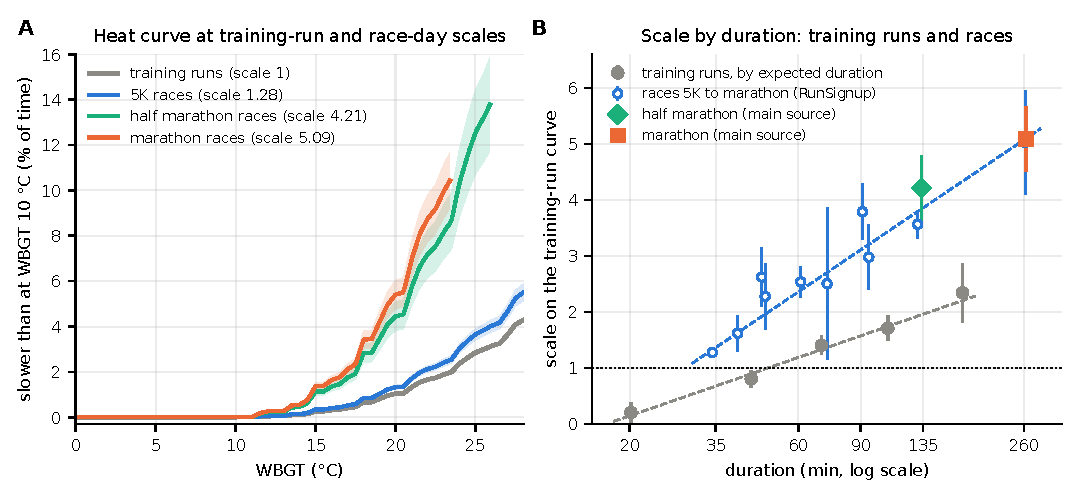
\includegraphics[width=\linewidth]{fig1_dose_response.pdf}
\caption{Training-run dose--response and race-day scale. \textbf{A}, the training-run heat curve \cW, the median runner's pace relative to WBGT 10\degC{} in counterfactual WBGT sweeps of the trained transformer (grey; zero at and below 10\degC), and the same curve multiplied by the race-day scales estimated from official results for the 5K (blue), the half marathon (green) and the marathon (orange); shaded bands are 95\% CI of the scale, and half-marathon and marathon curves are drawn up to the hottest edition in each set. \textbf{B}, within-runner scale on \cW{} for training runs in five bands of expected duration (grey; points at the band median; 95\% CI clustered by runner and by date and country; \nLtThirty, \nThirtySixty, \nSixtyNinety, \nNinetyOneFifty{} and \nGtOneFifty{} runs), race-day scales of ten distances from 5\,km to the marathon in the short-race source (open blue; course-clustered 95\% CI), and the half-marathon and marathon scales from the main official-results source (filled), placed at the median edition finish time. Dashed lines: fits on log duration across the training bands and across the ten race distances; dotted line: scale 1.}
\label{fig:dose}
\end{figure}

\begin{figure}[p]
\centering
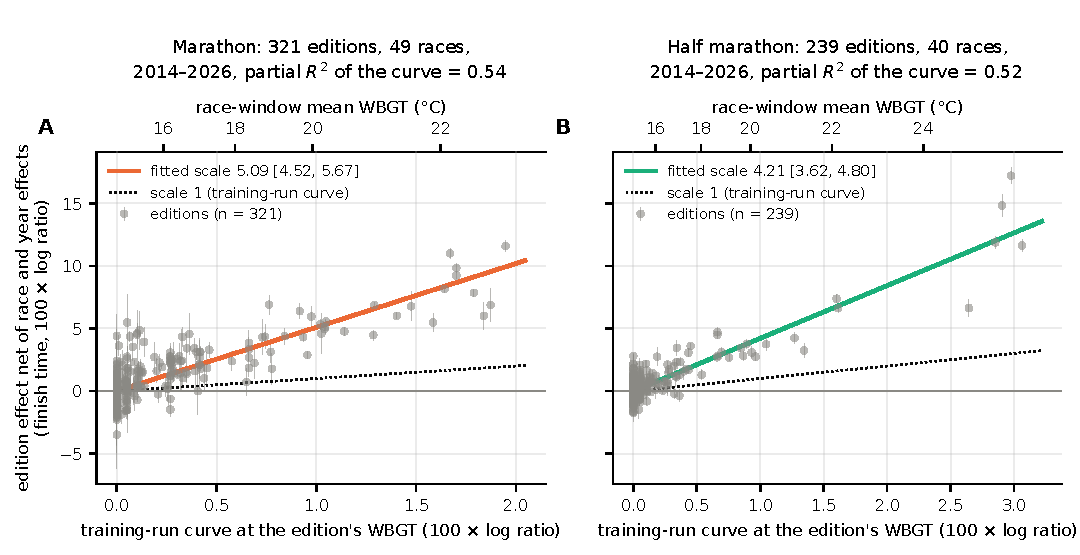
\includegraphics[width=\linewidth]{fig2_raceday_scale.pdf}
\caption{Within-person edition effects against the training-run curve at each edition's race-window WBGT. \textbf{A}, marathon, \nEdMar{} editions of \nRacesMar{} races; \textbf{B}, half marathon, \nEdHalf{} editions of \nRacesHalf{} races; 2014 to 2026 without 2020. Each point is an edition effect net of course and calendar-year fixed effects ($100 \times$ log ratio of finish time) with a 95\% CI from person-clustered standard errors. Solid line: fitted race-day scale (weighted least squares, weights $1/\mathrm{SE}^2$); dotted line: scale 1. The top axis gives the race-window mean WBGT corresponding to each curve value. Race-window WBGT is the mean from the first mass start to that start plus the edition's median finish time, at the start line. Panel titles give the partial $R^2$ of the curve beyond the fixed effects.}
\label{fig:raceday}
\end{figure}

\begin{figure}[p]
\centering
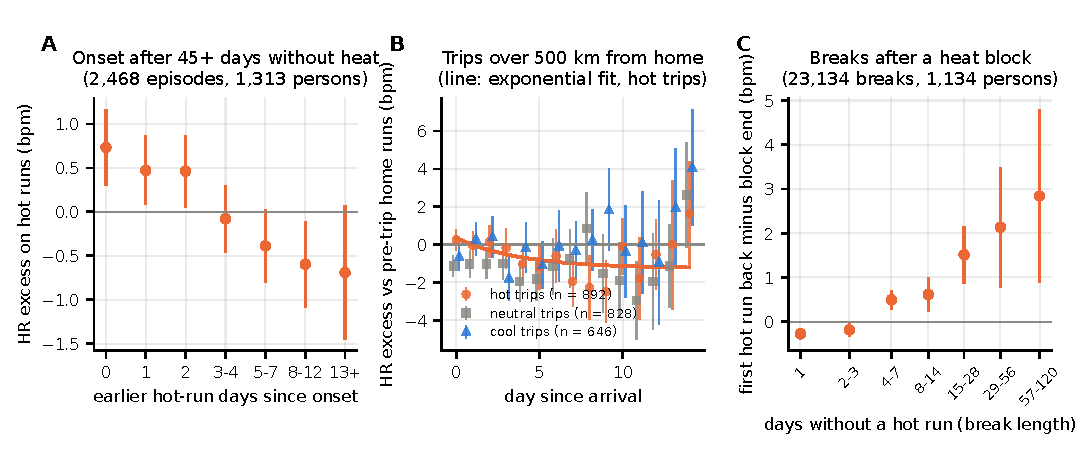
\includegraphics[width=\linewidth]{fig3_acclimation_kinetics.pdf}
\caption{Build and decay of heat acclimation in HR at matched load. The outcome is HR minus each runner's load model (pace, duration, climb), the start-hour effect and the population heat cost, relative to each design's baseline; heat is counted from WBGT 22\degC. \textbf{A}, onset: excess on hot runs by the number of earlier hot-run days after a first hot run that followed 45 or more days without one (episode fixed effects, days-since-onset trend, control for a hot run the day before; \kinOnsetEpisodes{} episodes). \textbf{B}, trips more than 500\,km from home: excess on away runs relative to home runs in the 45 days before the trip, by day since arrival, for hot ($\geq$5\degC{} warmer than home), neutral (within 2\degC) and cool ($\geq$5\degC{} cooler) trips; line, exponential fit to hot trips. \textbf{C}, breaks after a block of at least four hot-run days in 14: excess on the first hot run back minus the block's last week, by break length (\kinBreaks{} breaks). Means or coefficients with 95\% CI (person-clustered in A and C).}
\label{fig:kinetics}
\end{figure}

\begin{figure}[p]
\centering
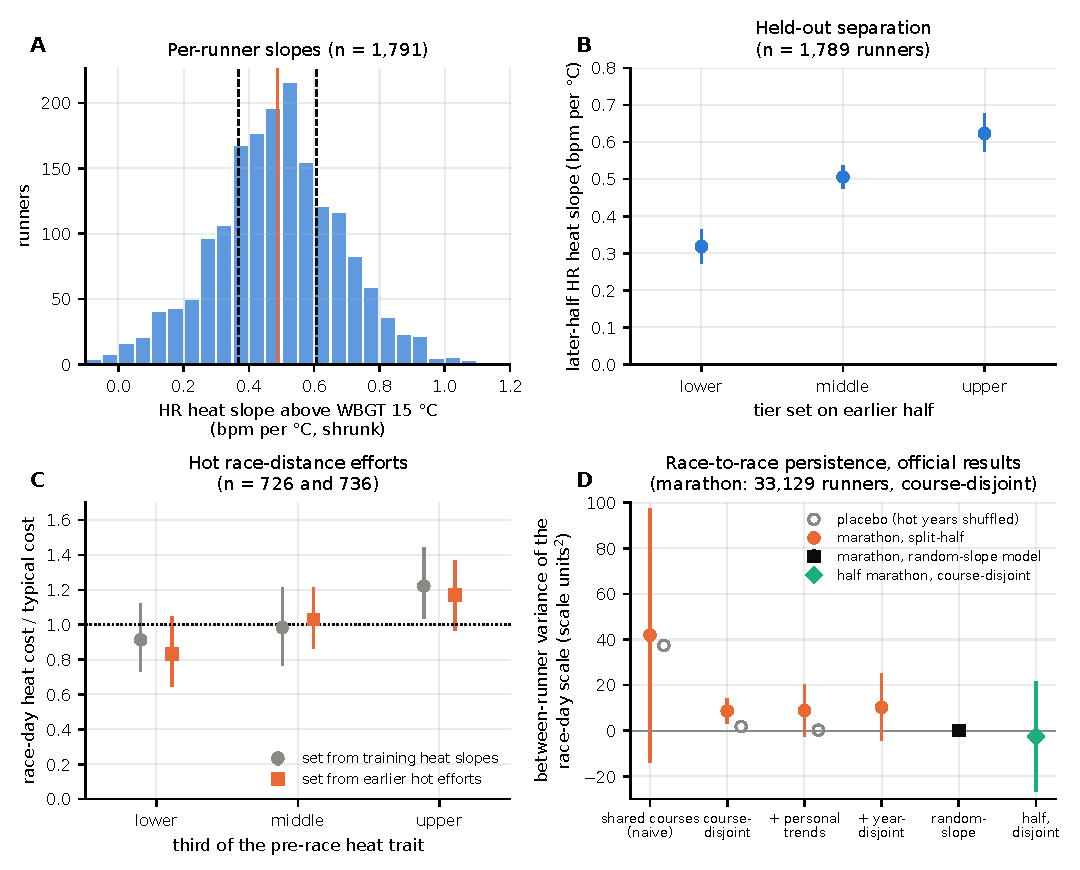
\includegraphics[width=\linewidth]{fig4_between_runner.pdf}
\caption{Between-runner differences in heat sensitivity in training and on race day. \textbf{A}, empirical-Bayes-shrunk HR heat slopes above WBGT 15\degC{} (\nSlopePersons{} runners); orange line, mean of the person slopes (\muPersons{} \bpmC); dashed lines, cut-points of three equal-probability tiers of the estimated true-slope distribution (\tierCuts{} \bpmC). \textbf{B}, later-half HR heat slope (mean and 95\% CI) by tier formed on the earlier half of each runner's history (\nTierRunners{} runners). \textbf{C}, race-day heat cost of hot race-distance efforts (WBGT 18\degC{} or above) by runners with at least one earlier hot effort, as a multiple of the population-typical cost after removing the runner's personal miss estimated from earlier data, by thirds of the training-derived heat trait (grey, \nTrainThirds{} efforts) or of the heat trait estimated from earlier race-distance efforts in the placement model (orange, \nEarlierThirds{} efforts); thirds use only data dated before each effort; 95\% CI from resampling runners; dotted line, typical cost. \textbf{D}, between-runner variance of the race-day scale in official results, estimated as the covariance of each runner's heat slopes from two halves of their races (95\% CI, delete-one-course jackknife): marathon halves sharing courses (naive), sharing no course, with personal trends, and sharing no calendar year; hollow markers, placebo with hot years shuffled within course; square, random-slope model on all repeat marathoners (upper bound shown); diamond, half marathon with halves sharing no course.}
\label{fig:between}
\end{figure}

\end{document}
" drops the line
% numbers; tables and figures already sit after the references, outside the counted span
\ifdefined\wordcountbuild
  \AtBeginDocument{\let\linenumbers\relax}
\fi

\begin{document}

% =====================================================================================================================
% TITLE PAGE
% =====================================================================================================================
\begin{titlepage}
\begin{flushleft}
{\Large\bfseries The performance cost of environmental heat in recreational distance runners: from within-runner training data to official race results\par}
\vspace{1.2em}
\textbf{Running head:} Heat cost from training to race day\par
\vspace{1.2em}
Peter Dunphy, Thomas Mulc, Gabe Cupino\par
\vspace{0.4em}
Kailo, Mountain View, CA, USA\par
\vspace{1.4em}
\textbf{Corresponding author:} \placeholder{name, postal address, e-mail address and telephone of the corresponding author}\par
\vspace{1.4em}
\textbf{Word count:} abstract \wcAbstract{} words; main text \wcMain{} words (Introduction to Conclusions, excluding the key-points box, references, tables and figure legends)\par
\textbf{Tables:} 2\quad \textbf{Figures:} 4\par
\vspace{1.4em}
\textbf{Extended version:} full methods and additional analyses are given in reference \citenum{dunphy2026extended}.\par
\vspace{1.4em}
{\small\textcolor{otred}{Working draft. Red brackets mark items to be supplied by the authors.}\par}
\end{flushleft}
\end{titlepage}

% =====================================================================================================================
% ABSTRACT
% =====================================================================================================================
\begin{onehalfspace}
\section*{Abstract}
\noindent\textbf{Purpose:} To quantify the performance cost of environmental heat in recreational runners, from training to race day, and to examine heat acclimation and between-runner differences.

\noindent\textbf{Methods:} We analysed \nRuns{} GPS-recorded training runs (\nRunners{} runners) and official results of 5-km to marathon races, computing wet-bulb globe temperature (WBGT) along each run and race window. A training-run heat curve was scaled within runner by expected duration and against within-person edition effects. Secondary outcomes were heart rate (HR) at matched load and individual differences.

\noindent\textbf{Results:} Versus 10\degC, training pace slowed at most \cFourteen\% up to WBGT 14\degC{} and \cTwentyeight\% at 28\degC; the within-runner scale rose from \scLtThirtyPt{} (runs under 30\,min) to \scGtOneFiftyPt{} (over 150\,min). Race-day scales rose with race duration, from \alphaFiveK{} (5K; 95\% CI) to \alphaHalfCI{} (half marathon) and \alphaMarCI{} (marathon), about \ratioRound{} the training scale at matched duration: \marMinTwenty{} min for a 4:00 marathon at WBGT 20\degC. In the heat, excess HR at matched load halved within \kinOnsetHalf{} hot-run days and returned with a half-life of \kinDecayHalf{} days without heat. Runners differed persistently in training HR heat slope (SD \sdPersistent{} \bpmC; at most three tiers), but this did not predict race-day heat cost, which was barely repeatable between races (reliability of a runner's race history about \persistRel).

\noindent\textbf{Conclusions:} Heat costs recreational runners more the longer the race, and about \ratioRound{} as much as training runs of equal duration.

\vspace{0.6em}
\noindent\textbf{Keywords:} wet-bulb globe temperature; heat acclimatization; marathon; half marathon; heart rate; wearable sensors
\end{onehalfspace}

\vspace{1em}
\begin{tcolorbox}[colback=white,colframe=black,boxrule=0.6pt,arc=0pt,left=6pt,right=6pt,top=4pt,bottom=4pt,title=Key points,coltitle=black,colbacktitle=gray!15,fonttitle=\bfseries]
\begin{itemize}[leftmargin=1.2em,itemsep=2pt,topsep=2pt]
\item Within the same recreational runners, the pace cost of heat on training runs was close to zero up to a WBGT of about \flatToWBGT\degC{}, accelerated above it, and grew with the duration of the run.
\item In official results, finish times followed the same curve at a scale rising with race duration, from about \alphaFiveKRound{} for the 5K to about \alphaMarRound{} for the marathon, about \ratioRound{} the cost of training runs of the same duration: \marMinTwenty{} min for a 4:00 marathon at WBGT 20\degC.
\item Heat acclimation was visible in HR at matched load, building within about \kinBuildRound{} hot runs and fading over one to two weeks without heat; runners differed persistently in their training HR response to heat (at most three groups), but neither this nor race history sorted runners reliably by race-day heat cost.
\end{itemize}
\end{tcolorbox}

\newpage
\doublespacing
\linenumbers

% =====================================================================================================================
\section{Introduction}
% =====================================================================================================================
Heat is among the most consistent environmental limits on endurance performance. During running most metabolic energy is released as heat; when the environment cannot remove it fast enough, skin blood flow competes with working muscle for cardiac output, sweat losses accumulate, and core temperature rises toward levels at which runners reduce their pace \cite{cheuvront2001,maughan2007,racinais2015}. The cost grows with the length of the event: across World Championships, sprint performances improved in the heat while endurance events were impaired by about 3\% \cite{guy2015art}. Because warming has made record heat more frequent \cite{king2017,russo2014}, more mass-participation races are run in conditions in which these limits bind.

Field estimates of the cost come mainly from race results, which show slowing that is small in cool conditions and grows with wet-bulb globe temperature (WBGT) \cite{ely2007,elhelou2012,knechtle2019,mantzios2022,vernon2021}. Most of these designs compare fields rather than people, so an edition's result also reflects who entered, started and finished; within-person designs have followed the same runners across three editions of one race \cite{tan2022}, elite athletes across races \cite{wang2024} and repeat finishers across North American marathons \cite{oliveira2026}. Controlled studies isolate the physiology and show that 5 to 14 days of heat exposure lower heart rate (HR) and core temperature at a fixed workload and improve performance in the heat \cite{periard2015,tyler2016art,tyler2024,james2017}, but they include tens of participants and rarely connect to race outcomes.

Wrist-worn GPS devices now record recreational runners' training in the conditions they actually meet, which allows within-runner comparisons of hot and cool days at scale. Large training-data studies have predicted race performance without weather \cite{smyth2020,emig2020benchmark}, and a model of wearable workouts has learned environmental effects on HR \cite{nazaret2023}, but we found no estimate of the pace cost of heat from individuals' training records and no study comparing it with race day. It is unknown whether a heat cost estimated on training runs, when a runner can slow down, shorten the session or move it to a cooler hour, describes what heat does on race day, how quickly heat exposure changes the cost in free-living runners, and whether runners differ in heat sensitivity consistently enough to be told apart.

The primary aim was to quantify the performance cost of environmental heat in recreational runners, linking a within-runner dose--response on training runs to race-day finish times in official results from 5\,km to the marathon. The secondary aims were (i) to describe how heat acclimation builds and decays in HR at matched load, and how recent exposure relates to race-day cost, and (ii) to estimate how persistent and how measurable individual differences in heat sensitivity are, in training and on race day. Against this literature the study adds four estimates: a training-run heat curve learned without a parametric form from runners' own GPS streams, whose scale is then estimated against independent official results; the ratio of race-day to training-run heat cost across ten race distances; the build and decay of acclimation from natural experiments in routine wearable records; and the persistence of individual heat sensitivity in training together with its transfer to race day. Full methods and further analyses are reported in an extended version \cite{dunphy2026extended}.

% =====================================================================================================================
\section{Methods}
% =====================================================================================================================
\subsection{Study design}
This retrospective observational study had three components: within-runner analyses of GPS-recorded training runs, analyses of race-distance efforts by the same runners, and within-person analyses of official marathon and half-marathon results, all secondary uses of existing records (see Declarations).

\subsection{Data sources and participants}
\paragraph{Training runs.} The corpus comprised outdoor runs recorded on Garmin devices by users of a training platform who had connected their accounts and permitted research use of their data. A run was retained when its mean pace was above 2.5 and below 11.5\,min\,km$^{-1}$, its mean HR above 60 and below 210\,bpm and its run-averaged WBGT at or below 28\degC, and when every covariate used below was present. The pace and HR bounds remove sensor and GPS artefacts; the WBGT ceiling reflects sparse data above it; runs without GPS were not included. Accounts belonging to one person were merged for the between-runner analyses.

\paragraph{Race-distance efforts.} Runs of 20.9 to 21.6\,km or 41.68 to 43.45\,km, with a mean HR of at least 80\% of the runner's estimated maximum, at least 20 earlier runs with weather, and a pre-race finish-time prediction, were analysed as race-distance efforts. The prediction came from a fitness model that uses only earlier training (fastest-segment times over preceding windows) \cite{dunphy2026extended}. Race labels are not available, so these efforts include an unknown share of training runs at race distance.

\paragraph{Official results.} Finish lists of marathons and half marathons held from 2014 to 2026 were assembled from a public results service, excluding virtual and cancelled editions, 2020, editions listed only as a multi-day weekend, and editions whose date or first mass-start time could not be verified from an official page or a news report. Finishers were linked across editions on normalised name, sex and a birth-year interval, with hometown as a tie-breaker; disagreement with the service's persistent member identifier, where present, bounded the false-link rate. Races from 5\,km to 10 miles came from a second public results service (United States) that records each event's scheduled start, with finishers linked within a course in the same way.

\subsection{Environmental exposure}
Exposure was outdoor WBGT ($0.7\,T_{\mathrm{nwb}} + 0.2\,T_{\mathrm{g}} + 0.1\,T_{\mathrm{a}}$), computed with the thermofeel library \cite{brimicombe2022} from air temperature, dew point, wind speed and shortwave and direct radiation, with mean radiant temperature derived from the radiation fluxes and the solar zenith angle. For training runs, weather came from a self-hosted instance of the Open-Meteo service \cite{zippenfenig2023} (the finest model available, 15-min or hourly), sampled at the start, every 15\,min and at the finish, and each run was summarised by its time-weighted mean WBGT. For each race edition, the date came from the published schedule, the start time from official pages or news reports (first mass-start wave; scheduled start for short races), and hourly ERA5 reanalysis \cite{hersbach2020} at the start line (the race city's 0.25\textdegree{} cell for short races) was interpolated and averaged from the start to the start plus the edition's median finish time. Over this window, the rise in WBGT and the degree-hours above 22\degC{} were computed, and the deviation from recent climate was the window WBGT minus the mean over the same clock window on the 60 preceding days.

A runner's recent exposure was summarised by a heat-exposure index between 0 and 1, computed from earlier runs only and updated daily: it rises in proportion to heat-weighted running time (minutes weighted from 0 at WBGT 22\degC{} to 1 at 28\degC, divided by 60 and capped at 1 per day; gain 0.15 times this stimulus times the remaining capacity) and decays by 2.5\% per day, following published kinetics \cite{racinais2015,daanen2018art}. For finishers in the official results, the published hometown was geocoded to a 1\textdegree{} cell (at least 30 persons), and a decay-weighted (14-day half-life) home WBGT over the 60 days before each race was expressed relative to the course's 60-day pre-race value.

\subsection{Outcomes}
For training runs the outcome was $100 \times \ln(\text{mean pace})$, which approximates a percentage change. For official results it was the within-person edition effect, estimated per course from same-course repeat pairs as $\ln(t_b/t_a) = e_b - e_a + \text{age term}$, with person-clustered standard errors; editions with fewer than 30 repeat pairs were dropped, and no drift term was fitted because it is collinear with the edition contrasts (long-run change enters through calendar-year effects). HR at matched load was the run's mean HR adjusted for relative speed, 30-day pace and distance, duration, climb and start hour. For race-distance efforts the outcome was the loss, $100 \times \ln(\text{actual}/\text{predicted finish time})$, re-centred on cool efforts (WBGT below 12.5\degC) of other runners, and its ratio $\rho$ to the population-typical race-day heat cost.

\subsection{Statistical analysis}
\paragraph{Training-run heat curve.} The shape of the heat response was taken from a transformer network trained on 90\% of runners to predict pace from each runner's 30 most recent activities, each represented as 128-point streams of pace, HR, cadence, power, distance, altitude, cumulative climb and WBGT, with date, latitude and activity type \cite{dunphy2026extended}. Sweeping WBGT through the trained network with all other inputs held fixed gave each runner's predicted pace across conditions. The curve \cW{} combines the median of the runners' normalised response shapes (\curveShapeRunners{} runners) with the median sensitivity of a reference sample (\curveRefRunners{} runners); it is zero at and below WBGT 10\degC{} and held constant above 28\degC{} \cite{dunphy2026extended}. These samples include \curveShapeHoldout{} and \curveRefHoldout{} runners from the network's holdout; a curve built on fitting runners alone differs from it by at most \curveHoldoutDiff{} percentage points. The network received no constraint on shape. Every magnitude reported below was estimated by regression on \cW, so the curve enters as a fixed covariate and its scale is estimated.

\paragraph{Within-runner dose--response.} On training runs, $100 \ln(\text{pace})$ was regressed on \cW{} within runner, with a cold term $\max(0, 10 - W)$, log distance, climb per kilometre (clipped at 100\,m\,km$^{-1}$) and log 30-day pace, separately within five bands of expected duration (distance times 30-day pace: under 30, 30 to 60, 60 to 90, 90 to 150 and over 150\,min), with runner-by-band intercepts. Expected rather than actual duration was used because heat itself lengthens a run, and HR was omitted because heat raises it. Race-distance runs were removed and runners needed at least 20 runs. Standard errors were clustered by runner and by date and country. A continuous version interacted \cW{} with log expected duration. Effort was examined with a label fixed before the run (the runner's usual share of maximal HR on that weekday), in thirds within runner. To check that the design does not produce a gradient by itself, the estimator was applied to data simulated with one common scale.

\paragraph{Race-day scale.} Edition effects were regressed on course and calendar-year fixed effects and $\alpha\,c(\bar W)$, where $\bar W$ is the race-window WBGT, by weighted least squares (weights $1/\mathrm{SE}^2$), separately for each distance; marathons and half marathons were also fitted jointly with a distance interaction, short-race intervals were clustered by course, and the scales of ten distances were regressed on the log of median finish time. The coefficient $\alpha$ states how many times the training-run curve the race-day cost is; dividing it by the training scale of the matching duration band gave a race-to-training factor (delta method). Fit is reported as the partial $R^2$ of the curve beyond the fixed effects, because the overall $R^2$ includes the calendar trend absorbed by the year effects. Robustness analyses used quantiles of the within-person deviations, finish-time tiers assigned from each runner's other finishes (so that tiers are not built from the outcome), a free piecewise-linear shape compared by leave-one-race-out cross-validation, and the WBGT rise and degree-hours as added terms. Official split times gave the share of the heat cost incurred in the second part of the race.

\paragraph{Recent heat exposure.} (a) Kinetics: the HR excess was a run's HR minus a within-person load model fitted on cool runs (log pace, log duration, climb), the start-hour effect and the population heat cost, on runs of at least 20\,min; a hot run lasted at least 20\,min at WBGT 22\degC{} or above. Three natural experiments used it. Onset: the first hot-run day after 45 or more days without one, with the excess on hot runs modelled by the number of earlier hot-run days (episode fixed effects, a days-since-onset trend, a control for a hot run the day before) and compared with calendar days and ambient heat by person bootstrap. Trips: runs more than 500\,km from a rolling home, classed as hot ($\geq$5\degC{} warmer than nearby home runs), neutral (within 2\degC) or cool ($\geq$5\degC{} cooler), with the excess relative to home runs in the 45 preceding days regressed on days since arrival (trip fixed effects). Breaks: after at least four hot-run days in 14, the first hot run back was compared with the block's last week, by break length. Exponential fits gave half-lives, and a recursive state (gain proportional to remaining capacity, first-order decay) was fitted by profile likelihood with a future-dose placebo. (b) Race-distance efforts: the exposure index entered the placement model below. (c) Official results: the positive deviation from recent climate was added to the edition regression, and in the hometown design $\ln(\text{finish time})$ was regressed on person and edition fixed effects and the interaction of $c(\bar W)$ with recent home climate (percent of finish time per percentage point of curve per \textdegree C), clustered by person.

\paragraph{Between-runner differences.} Each person's HR heat slope above WBGT 15\degC{} was estimated in the matched-load model (persons with at least 10 runs above 15\degC). Because errors of consecutive runs are correlated, the true between-person variance was estimated as the covariance of slopes from disjoint halves of each history: alternate calendar weeks, early against late history (the persistent part), and odd against even heat seasons. The persistent variance explained by proxies (body mass from active energy per kilometre, a stride-based height proxy, maximal HR, fitness, volume) was cross-fitted over five folds of persons, and empirical-Bayes-shrunk slopes were cut into three, four or five equal-probability tiers on the early half of each history and evaluated on the late half. Race-day placement used a linear mixed model of the loss with two effects per runner, a personal miss against the prediction that applies at every temperature and a heat trait (a multiple of the typical cost), with the exposure index and 28-day volume in the heat term and an optional training-derived prior for the trait. It was fitted by restricted maximum likelihood on four of five runner folds, each held-out effort's runner effects coming from that runner's earlier efforts only; the correlation between the two effects was fixed at zero after inspection. Pre-specified comparisons added earlier efforts, the training-derived trait and the exposure index to a population model, judged by the mean absolute error of predicted loss on hot efforts (WBGT at or above 18\degC) with runner-bootstrap intervals. Persistence of the race-day scale in official results was estimated by splitting each runner's editions into two halves that shared no course, each with warm (WBGT 15\degC{} or above) and cool editions; within each half, edition-adjusted log finish time was regressed on the curve value relative to the course mean, and the precision-weighted covariance of the two slopes estimated the persistent between-runner variance, with delete-one-course jackknife intervals and placebos that shuffled heat within runner or across years within course.

\paragraph{Inference.} Estimates are reported with 95\% confidence intervals (CI), from cluster-robust standard errors or from bootstrap resampling of runners, persons or race dates, as detailed in the extended version \cite{dunphy2026extended}. The within-runner training scale by duration and $\alpha$ for each distance were designated primary. All other analyses are secondary, were not adjusted for multiplicity, and their intervals should be read as descriptive; $p$ values are given only for key contrasts. Analyses used Python with statsmodels, scikit-learn and JAX.

% =====================================================================================================================
\section{Results}
% =====================================================================================================================
\subsection{Cohorts}
The corpus held \nRuns{} runs by \nRunners{} runners (median \runsPerRunnerMed{} runs per runner, interquartile range \runsPerRunnerIQR) recorded from \corpusFirst{} to \corpusLast{} in \nCountries{} countries (Table~\ref{tab:cohorts}). Median run WBGT was \wbgtMed\degC{} (10th to 90th percentile \wbgtPten{} to \wbgtPninety\degC); \shareEighteen\% of runs took place at 18\degC{} or above and \shareTwentytwo\% at 22\degC{} or above. There were \nEfforts{} race-distance efforts (\nEffHalf{} half, \nEffMar{} marathon) by \nEffRunners{} runners, \nEffHot{} of them at WBGT 18\degC{} or above (\nEffHotRunners{} runners). The official results comprised \nFinishes{} finishes by \nPersons{} persons, \nRepeaters{} of whom finished twice or more, and edition effects were estimable on \nCoursesEff{} courses. After exclusions (\nNoStart{} held editions outside 2020 lacked a sourced first mass-start time), \nEdMar{} marathon editions of \nRacesMar{} races and \nEdHalf{} half-marathon editions of \nRacesHalf{} races, with \nFinAnalysis{} finishes, entered the analysis. Their race-window WBGT ranged from \wbgtRangeMar\degC{} for marathons (\edMarEighteen{} editions at 18\degC{} or above, \edMarTwentytwo{} at 22\degC{} or above) and from \wbgtRangeHalf\degC{} for half marathons (\edHalfEighteen{} and \edHalfTwentytwo). The member identifier disagreed with the linkage for \falseLink\% of the persons on whom it could be checked.

\subsection{Training-run dose--response}
The training-run curve was close to zero up to WBGT 14\degC{} (\cFourteen\%) and then rose at an increasing rate, to \cSixteen\% at 16\degC, \cTwenty\% at 20\degC, \cTwentyfour\% at 24\degC{} and \cTwentyeight\% at 28\degC, relative to 10\degC{} (Fig.~\ref{fig:dose}A). Within runner, the scale on this curve increased with expected run duration, from \scLtThirty{} for runs under 30\,min (\nLtThirty{} runs) to \scThirtySixty{} (30 to 60\,min), \scSixtyNinety{} (60 to 90\,min), \scNinetyOneFifty{} (90 to 150\,min) and \scGtOneFifty{} for runs over 150\,min (\nGtOneFifty{} runs by \nGtOneFiftyRunners{} runners) (Fig.~\ref{fig:dose}B). Across the bands the scale rose by about \trainPerDoubling{} per doubling of duration. Applied to data simulated with one common scale of \placeboTrue, the estimator returned \placeboRange{} in every band. With effort fixed before the run, hard days were not steeper than easy days (difference \effortGradient\% per \textdegree C). At WBGT 20\degC, a training run of over 150\,min was therefore \longTwenty\% slower than at 10\degC{} (Table~\ref{tab:cost}).

\subsection{Race-day scale in official results}
Within-person edition effects rose with the value of the training-run curve at each edition's WBGT (Fig.~\ref{fig:raceday}). The race-day scale was $\alpha$ = \alphaMarCI{} for the marathon (partial $R^2$ of the curve \prsqMar) and \alphaHalfCI{} for the half marathon (\prsqHalf), a difference of \alphaDiff{} ($p$ = \alphaDiffP). Relative to training runs of matching duration, the race-day cost was \ratioMar{} times larger for the marathon and \ratioHalf{} times larger for the half marathon (Fig.~\ref{fig:dose}B). At a race-window WBGT of 21\degC{} a marathon took \marPctTwentyone\% longer than at 10\degC, \marMinTwentyone{} min on a 4:00 finish. Table~\ref{tab:cost} converts the scales into finish time across distances and conditions; at WBGT 20\degC{} a 4:00 marathon was \marMinTwenty{} min slower than at 10\degC. In official results of shorter races the scale was \alphaFiveK{} for the 5K (\nEdFiveK{} editions of \nCrFiveK{} races, \nWarmFiveK{} at WBGT 18\degC{} or above), \alphaTenK{} for the 10K (\nEdTenK{}, \nCrTenK{}, \nWarmTenK) and \alphaFifteen{} for 15\,km and 10 miles pooled (\nEdFifteen{}, \nCrFifteen{}, \nWarmFifteen; \alphaFifteenNoBoiler{} without the race with the largest weight). Across ten distances from 5\,km to the marathon, $\alpha$ = \durIntercept{} + \durSlope{}\,ln(median finish time, min) (weighted $R^2$ \durRsq), about \durPerDoubling{} per doubling of race duration against \trainPerDoubling{} for training runs, so races cost \raceOverTrainRange{} times the training scale at matched duration (Fig.~\ref{fig:dose}B). In this source the marathon scale was \rsuMar{} and the half-marathon scale \rsuHalf{}; shifting every start by one hour changed the scale by \startShift\%. Within each distance, the scale was highest for mid-pack finishers and lower for the fastest and slowest.

The scale did not depend on a minority of runners who slowed markedly. Estimated on the median of each edition's within-person deviations it was \alphaMarMedian{} for the marathon and \alphaHalfMedian{} for the half marathon; on the 25th percentile, \alphaMarQtf{} and \alphaHalfQtf. Finish-time tiers assigned from each runner's other finishes showed no linear trend in the marathon (\tierMarTrend{} per hour) or half marathon (\tierHalfTrend). A free piecewise shape rose earlier than the scaled curve (\freeFourteen{} against \scaledFourteen{} log points at WBGT 14\degC, marathon) but lowered leave-one-race-out error only from \rmseScaled{} to \rmseFree{} (\rmseNoWx{} without weather).

At matched mean WBGT, each degree of rise over the race window added \riseMar\% of finish time in the marathon and \riseHalf\% in the half marathon (pooled \risePooled\%). Degree-hours above 22\degC, non-zero in \nDhMar{} marathon and \nDhHalf{} half-marathon editions, were not distinguishable from zero alongside the curve (\dhMar{} and \dhHalf\% per \textdegree C\,h). In official split times (\nSplitRunners{} runners in \nSplitEd{} editions of \nSplitCourses{} courses), \lateShare\% of the heat cost in the \nSplitWarm{} warm editions fell in the second part of the race.

\subsection{Recent heat exposure}
At matched load, HR rose by \hrSlope{} \bpmC{} above WBGT 15\degC{} plus \hrSlopeTwentyfour{} above 24\degC{} (\hrRuns{} runs, \hrPersons{} persons), and this cost was larger before acclimation (Fig.~\ref{fig:kinetics}). After 45 or more days without heat (\kinOnsetEpisodes{} episodes, \kinOnsetPersons{} persons), the excess fell by \kinOnsetDecline{} bpm, half of it within \kinOnsetHalf{} hot-run days. On hot trips (\kinTrips{} trips, \kinTripPersons{} runners) the half-life was \kinTripHalf{} days and the excess declined by \kinSlopeHot{} bpm per day over the first week, against \kinSlopeNeutral{} on neutral (\kinTripsNeutral) and \kinSlopeCool{} on cool trips (\kinTripsCool); the arrival level (about \kinArrival{} bpm above neutral trips) depends on the baseline used. The count of hot-run days described the build better than calendar days (\kinCountCal\% of bootstraps) or ambient heat (\kinCountAmb\%), neither of which added to it (\kinCalAdd{} and \kinAmbAdd{} bpm). After a block of hot running (\kinBreaks{} breaks, \kinBreakPersons{} persons), the first hot run back carried \kinBreakFour, \kinBreakEight, \kinBreakFifteen{} and \kinBreakTwentynine{} bpm more excess after 4--7, 8--14, 15--28 and 29--56 days off, a decay half-life of \kinDecayHalf{} days; state models gave \kinStateOnset{} and \kinStatePanel{} days. On \kinNonhotBreaks{} breaks with non-hot runs at both ends, the hot-run rise exceeded the non-hot rise by \kinNonhotDiD{} bpm at 15--28 days, so up to about a third of the rise was not specific to heat. Saturation was not identified, and a shift in HR at every WBGT failed the future-dose placebo.

In the placement model, each unit of the exposure index changed the race-day heat cost by \scoreRace{} times the typical cost (28-day volume \volumeRace{} per SD). In official results, each degree by which race-window WBGT exceeded the 60-day climate added \devMar\% of finish time in marathons and \devHalf\% in half marathons. A warmer recent home climate went with a smaller heat cost, by \homeMarAlone{} percent of finish time per percentage point of curve per \textdegree C in marathons (\homeFinMar{} finishes, \homePersMar{} persons, \homeEdMar{} editions) and \homeHalfAlone{} in half marathons (\homeFinHalf, \homePersHalf, \homeEdHalf); for a marathon at WBGT 22\degC, a home climate 5\degC{} warmer than the course corresponds to \homeIllusMar\% (\homeIllusMarMin{} min on 4:00).

\subsection{Between-runner differences}
The true between-person SD of the HR heat slope was \sdPersistent{} \bpmC{} between the early and late halves of each history (\nSlopePersons{} persons) and \sdSeasons{} between different heat seasons (\nSeasonsPersons{} persons), against a population slope of \hrSlope. The persistent part made up \sharePersistent\% of the systematic between-person variance, the remaining \shareSameSeason\% varying within a season, and \acrossSummers\% of the alternate-week variance persisted across summers. The split-half reliability of a slope estimated from a full history was \reliability. The proxies jointly explained \proxyShare\% of the persistent variance, and the body-mass proxy \massShare\%.

Three tiers formed on the early half of each history separated later-half slopes of \tierLate{} \bpmC{} (upper minus lower \tierGap; \nTierRunners{} runners; Fig.~\ref{fig:between}A,B). The median runner's posterior probability of belonging to the assigned tier was \postThree\% with three tiers, \postFour\% with four and \postFive\% with five.

On the \nEffHot{} hot race-distance efforts (\nEffHotRunners{} runners), the held-out mean absolute error of the population model was \cpMissPop{} percentage points of finish time. The training-derived trait did not change it (\cpTrainPrior), the runner's earlier race-distance efforts reduced it by \cpRaces{} (to \cpRacesVal), and these with the exposure index by \cpCombined{} (to \cpCombinedVal). Most of the gain came from the personal miss, which applies at every temperature; the heat-specific part alone gave \cpHeatOnly. Among runners with an earlier hot effort, thirds of the estimated trait had race-day heat costs of \groupsEarlier{} times typical (upper minus lower \gapEarlier), against \groupsTrain{} (\gapTrain) for thirds of the training-derived trait (Fig.~\ref{fig:between}C), but the median posterior probability of the most probable third was only \postOneRace{} after one earlier hot effort and \postFiveRaces{} after five or more. \shareNoEarlier\% of hot efforts had no earlier hot effort; among these, training-derived thirds differed by \gapNoEarlier. Fixing the personal-miss and trait correlation at zero left the held-out error unchanged.

In official results, race-day heat cost showed little persistence between races (Fig.~\ref{fig:between}D). With marathon races split into halves sharing no course (\persistRunners{} runners, effective sample \persistNeff), the between-runner variance of the race-day scale was \persistTau{} (one-sided $p$ = \persistP), \persistTauPlacebo{} after subtracting the placebo, an SD of \persistSD{} scale units (\persistPct\% of finish time at WBGT 21\degC). The estimate was fragile: with personal trends it was \persistTrend, with halves that also shared no calendar year \persistYear, and a random-slope model fitted to all \nRepeatMar{} repeat marathoners placed it at zero (upper bound \remlUpper). A naive split sharing courses gave \naiveTau, of which shuffling hot years within course reproduced \naiveP. A runner's whole race history measured the scale with reliability \persistRel{} (90th percentile \persistRelPninety); thirds assigned from it would be right for \persistTercile\% of runners against 33\% by chance, and one earlier hot race at WBGT 21\degC{} would move the forecast for the next by about \persistShrink{} of its excess. General form persisted (correlation of cool-race levels between halves \formCorr), the warm-minus-cool contrast did not (\contrastCorr). In half marathons persistence was not identified (\persistHalf; \persistHalfRunners{} runners). Women (\womenScale) and runners finishing under 3:00 (\subThreeScale) had lower scales.

% =====================================================================================================================
\section{Discussion}
% =====================================================================================================================
\subsection{Principal findings}
On training runs, the cost of heat was negligible up to a WBGT of about \flatToWBGT\degC{} and then accelerated, and within the same runners it grew with the duration of the run. In official results, within-person finish times followed approximately the same curve at a scale rising with race duration, from about \alphaFiveKRound{} for the 5K to about \alphaMarRound{} for the marathon, roughly \ratioRound{} the cost of training runs of the same duration. Heat acclimation was visible in HR at matched load, building over about \kinBuildRound{} hot-run days and fading with a half-life of about \kinDecayRound{} days, and recent heat exposure was associated with a smaller race-day cost. Runners differed persistently in their HR response to heat in training, but race-day heat cost showed little detectable persistence between races, and the gain from a runner's earlier races came mostly from their general standing rather than from heat.

\subsection{Comparison with previous work}
The flat-then-accelerating shape agrees with syntheses of elite racing, in which performance was stable up to about 15\degC{} WBGT and declined above it \cite{mantzios2022}, and with mass-field marathon analyses \cite{ely2007,elhelou2012,knechtle2019}; the race-day response began at a lower WBGT than the scaled training curve, consistent with optimal marathon air temperatures of about 4 to 12\degC{} \cite{elhelou2012,maughan2010,llewellyn2025}. The magnitudes are of the order reported for mass fields: in seven North American marathons the 50th finisher slowed by 3.5\% between the coolest and warmest WBGT quartile and the 300th by 7.9\% \cite{ely2007}, and surveyed finishers of the warm 2018 London Marathon reported times about 14\% slower than they had expected \cite{vernon2021}. Like other within-person designs \cite{tan2022,guo2019,oliveira2026}, the present estimates compare the same people across editions, so changes in who enters or finishes affect them less; they add weather over each edition's race window from a sourced start time, a range of distances, and a scale relative to the training curve.

The dependence on duration agrees with championship data, in which endurance events were impaired and sprints were not \cite{guy2015art}, with larger losses of slower half-marathon finishers attributed to their longer exposure \cite{hodgson2022}, and with laboratory evidence that heat decrements grow as running is prolonged \cite{periard2015self,hunter2026}; it quantifies that ordering across recreational races from 5\,km upward and within individual runners' training. Elite discipline-specific slopes are not monotone in duration \cite{mantzios2022}, so the ordering may not hold at elite intensity. Duration and intensity were not separated: within a distance, mid-pack finishers lost the most and the fastest and slowest less, so the gradient across distances is not a pure effect of time on course. Earlier studies disagree on who loses most within a distance: slower runners in designs that compare finishing places \cite{ely2007,vihma2010}, faster runners in others \cite{gasparetto2020,oliveira2026,inoue2026}. The back-loading of the race-day cost agrees with marathon pacing data in which the gap between closing and opening 5-km pace widened with temperature \cite{ely2008}, with a within-runner analysis in which the penalty fell mostly in the second half \cite{oliveira2026}, and with laboratory evidence that running speed falls once core temperature approaches about 39\degC{} part-way through a hot half marathon \cite{rodrigues2020}.

The HR kinetics resemble those of controlled acclimation. Half of the build came within about \kinBuildRound{} hot-run days, as in induction studies in which the HR reduction develops most rapidly over 4 to 5 days and is virtually complete after 7 \cite{periard2015,pandolf1998}, and it followed the number of exposures rather than elapsed time or ambient heat, as in laboratory comparisons of exposure schedules \cite{willmott2018,stevens2025}. Its size, \kinOnsetDecline{} bpm, is about a tenth of the reductions measured in standardised heat-stress tests, which impose a larger and fixed heat load. The decay half-life of about \kinDecayRound{} days is close to the 60\% loss of the HR adaptation over 14 days in a laboratory decay study \cite{flouris2014}, and its interval includes the meta-analytic loss of 2.3\% per day \cite{daanen2018art}; core-temperature and sweating adaptations decay more slowly \cite{weller2007,poirier2015}, and a residual benefit of months of natural acclimatisation \cite{malgoyre2020} would not be visible within the break windows used here. Part of the rise after a break is consistent with the higher exercise HR of short-term detraining \cite{mujika2000}. The exposure index used on race-distance efforts decays at the literature rate. The added cost of a race warmer than the preceding weeks agrees with the London Marathon differential \cite{vernon2021}, and the hometown association with the advantage of athletes from warmer countries in a desert ultramarathon \cite{ioannou2018}.

Individual variation in laboratory heat strain and acclimation is well documented \cite{mee2015,corbett2018}, but we are not aware of a peer-reviewed estimate of the persistence and reliability of an individual heat response in free-living athletes at this scale. The persistent between-runner SD of \sdPersistent{} \bpmC{} is large next to the population slope, yet body size, a source of differences in heat strain in laboratory studies \cite{marino2000,cramer2014}, explained almost none of it, consistent with the small share of heat strain that individual characteristics explain at relative intensities when evaporation is not limited \cite{havenith1998,jay2011}. Most training runs are in compensable conditions, where that mechanism is weakest, and the mass proxy is indirect, so this concerns the proxy rather than body mass. On race day, at most about \persistSpreadShare{} of the extra spread of finish times in heat was persistent, so the stable HR difference seen in training is not, in these data, a usable measure of an individual's race-day heat tolerance; we found no earlier estimate of whether an individual's race-day heat cost repeats. Group differences, such as the lower scale of women and of the fastest runners, were more robust. A smaller heat effect in women agrees with some mass-field analyses \cite{vihma2010,trubee2014} but not others \cite{knechtle2021b,wang2024}, and the lower scale of the fastest runners runs against a within-runner analysis of North American marathons \cite{oliveira2026}.

\subsection{Mechanisms}
Three features of racing plausibly make heat cost more than in training of the same duration. First, a race is run close to the highest sustainable output: in training part of the heat strain is absorbed as a higher HR at an unchanged pace, whereas at race intensity it has to be paid in pace \cite{cheuvront2001,periard2015}. Second, a race fixes the distance, date and start time, while in training a runner can shorten, slow down or move to a cooler hour, the behavioural thermoregulation that dominates self-paced exercise in heat \cite{flouris2015,junge2016}, which attenuates the training estimate. Third, race pace is set in advance and corrected late, which fits the back-loaded cost in the splits \cite{rodrigues2020}. The race-day scale therefore combines physiology with pacing and selection, and is not a purely physiological multiplier.

\subsection{Practical applications}
For a recreational marathoner, heat begins to cost time at a WBGT of about \costStartRange\degC{} and the cost rises quickly: about \marMinSixteen, \marMinEighteen, \marMinTwenty{} and \marMinTwentytwo{} min for a 4:00 runner at 16, 18, 20 and 22\degC, and less over shorter races (Table~\ref{tab:cost}). Slowing on hot training runs, even long ones, understates the race-day cost, so goals and pacing plans should follow the forecast race-window WBGT rather than training experience. The HR strain of heat eases after a few hot runs and the benefit fades over one to two weeks without heat, so hot running in the last weeks before a race, or arriving early, is what counts. Neither training data nor race history sorted individual runners reliably by race-day heat tolerance, so individual adjustments beyond the population scale are not supported by these data.

\subsection{Strengths and limitations}
Strengths are within-person designs on training and race data, which hold ability constant; race weather from each edition's official date, start and location; samples large enough to resolve the warm range; and independent sources analysed on a common heat curve. The design is observational, and the race-day scale absorbs pacing, field composition and selection; only finishers are observed, and withdrawals rise steeply with heat \cite{roberts2010}, so the scale is biased downward. The training-to-race factor divides a race-day scale from official-results finishers by a training scale from device users. Exposure comes from gridded weather fields rather than on-course measurement. Marathon editions reached a race-window WBGT of \wbgtMaxMar\degC, with \edMarTwentytwo{} at 22\degC{} or above, so costs beyond about 22\degC{} are extrapolations. The corpus consists of self-selected device users, and its race-distance efforts are not confirmed races. The curve comes from a learned model and $\alpha$ is a ratio to it, and a single scale only approximates the race-day shape. Short-race results are from the United States only, with weather at the race city. Linkage relies on names, HR was measured optically, sex was not observed in the corpus, secondary analyses were not adjusted for multiplicity, and one placement-model choice was made after inspection.

% =====================================================================================================================
\section{Conclusions}
% =====================================================================================================================
Environmental heat slows recreational distance runners little below a WBGT of about \flatToWBGT\degC{} and progressively more above it. The same curve, estimated within runners on training runs, describes race-day finish times in official results at a scale that rises with race duration, from about \alphaFiveKRound{} for the 5K to about \alphaMarRound{} for the marathon, roughly \ratioRound{} the cost of training runs of the same duration. Recent heat exposure reduces the HR cost of running in the heat within a few hot runs, a benefit that fades with a half-life of about \kinDecayRound{} days, and is associated with a smaller race-day cost. Runners differ persistently in their HR response to heat in training, but race-day heat cost is barely repeatable between races, so neither training data nor race history sorts individual runners reliably by race-day heat tolerance. What is new relative to earlier work is a heat curve learned from individuals' training records and tested on official results, the ratio of race-day to training cost across race distances, acclimation kinetics from routine wearable data, and a direct test showing that individual heat sensitivity measured in training does not carry to race day.

% =====================================================================================================================
\section*{Declarations}
% =====================================================================================================================
\paragraph{Ethics approval.} \placeholder{Ethics statement to be completed by the authors: name of the reviewing body and reference number, or the basis for exemption.} This study is a secondary analysis of de-identified training records held by a training platform and of finish lists publicly posted by race organisers and timing services. No individual is identifiable in any reported result.

\paragraph{Consent to participate.} \placeholder{Confirm the wording of the platform's research-use consent.} Platform users permitted research use of their data. Finishers in public results did not consent individually; only aggregate estimates are reported, and no names or individual results are reproduced.

\paragraph{Funding.} \placeholder{Funding statement.}

\paragraph{Competing interests.} \placeholder{Competing-interests statement to be completed.} All authors are affiliated with Kailo, the company whose training platform supplied the training-run data.

\paragraph{Data and code availability.} The training-run data contain location traces and cannot be shared publicly; \placeholder{access conditions}. Official results are publicly posted by race organisers; the person-linked tables derived from them are not shared because they are built from names. Analysis code and aggregate tables are available at \placeholder{repository}.

\paragraph{Author contributions (CRediT).} \placeholder{Conceptualization; Data curation; Formal analysis; Methodology; Software; Visualization; Writing, original draft; Writing, review and editing: to be assigned.}

\paragraph{Acknowledgements.} \placeholder{Acknowledgements.}

% =====================================================================================================================
\clearpage
\nolinenumbers
\singlespacing
\bibliographystyle{vancouver}
\bibliography{../references,../tommy_refs,journal_refs}

% =====================================================================================================================
% TABLES
% =====================================================================================================================
\clearpage
\begin{table}[p]
\centering
\caption{Characteristics of the three data sets. Values are counts or median (interquartile range) unless stated.}
\label{tab:cohorts}
\small
\renewcommand{\arraystretch}{1.25}
\begin{tabular}{@{}>{\raggedright\arraybackslash}p{2.9cm}>{\raggedright\arraybackslash}p{4.1cm}>{\raggedright\arraybackslash}p{3.6cm}>{\raggedright\arraybackslash}p{4.6cm}@{}}
\toprule
 & Training runs & Race-distance efforts & Official results \\
\midrule
Source & GPS wrist devices, users of a training platform & Subset of the training-run corpus & Public results service, marathons and half marathons \\
Period & \corpusFirst{} to \corpusLast & \corpusFirst{} to \effortsLast & 2014 to 2026 (2020 excluded) \\
Units & \nRuns{} runs by \nRunners{} runners; runs per runner \runsPerRunnerMed{} (\runsPerRunnerIQR) & \nEfforts{} efforts (\nEffHalf{} half, \nEffMar{} marathon) by \nEffRunners{} runners & \nFinishes{} finishes by \nPersons{} persons, \nRepeaters{} with two or more \\
Analysed subset & All runs; between-runner analyses: \nSlopePersons{} persons with 10 or more runs above 15\degC & WBGT 18\degC{} or above: \nEffHot{} efforts by \nEffHotRunners{} runners & Marathon: \nEdMar{} editions of \nRacesMar{} races, \finMar{} finishes; half marathon: \nEdHalf{} editions of \nRacesHalf{} races, \finHalf{} finishes \\
Distance, duration & \medDist{} km; \medDur{} min & 20.9--21.6 or 41.68--43.45\,km & Median edition finish time: marathon \medFinMar, half \medFinHalf{} (h:min) \\
Pace, heart rate & \medPace{} min\,km$^{-1}$; \medHR{} bpm & Mean HR 80\% of maximum or more & Not recorded \\
Exposure (WBGT) & Run mean \wbgtMed\degC{} (10th--90th percentile \wbgtPten--\wbgtPninety); \shareEighteen\% of runs at 18\degC{} or above, \shareTwentytwo\% at 22\degC{} or above & Run mean, as for training runs & Race-window mean: marathon \wbgtRangeMar\degC{} (\edMarEighteen{} editions at 18\degC{} or above, \edMarTwentytwo{} at 22\degC{} or above); half \wbgtRangeHalf\degC{} (\edHalfEighteen, \edHalfTwentytwo) \\
Weather source & Finest available model field, sampled every 15\,min along the run & As for training runs & ERA5 at the start line, first mass start to median finish \\
Outcome & $100\ln(\text{pace})$; HR at matched load & Loss against a pre-race prediction & Within-person edition effect \\
\bottomrule
\end{tabular}
\par\smallskip
\parbox{\linewidth}{\footnotesize Countries of training runs: \nCountries{} (United States \shareUS\%, South Korea \shareKR\%, United Kingdom \shareGB\%).}
\end{table}

\begin{table}[p]
\centering
\caption{Heat cost relative to WBGT 10\degC{} implied by the estimated scales: percent of time, with minutes on a reference finish time in parentheses (5K 0:30, 10K 1:00, 15\,km and 10 miles 1:30, half marathon 2:00, marathon 4:00).}
\label{tab:cost}
\small
\renewcommand{\arraystretch}{1.35}
\setlength{\tabcolsep}{5pt}
\begin{tabular}{@{}lccccc@{}}
\toprule
 & & \multicolumn{4}{c}{Race-window or run WBGT (\textdegree C)} \\
\cmidrule(lr){3-6}
 & Scale [95\% CI] & 16 & 18 & 20 & 22 \\
\midrule
Training runs, all & \TabTr \\
Training runs over 150\,min & \TabLong \\
5K & \TabFiveK \\
10K & \TabTenK \\
15\,km and 10 miles & \TabFifteen \\
Half marathon & \TabHalf \\
Marathon & \TabMar \\
\bottomrule
\end{tabular}
\par\smallskip
\parbox{\linewidth}{\footnotesize Scales multiply the training-run curve \cW; training runs over 150\,min use the within-runner scale of that expected-duration band; 5K to 10 miles use course-clustered intervals; half marathon and marathon use the main official-results source. Percentages are $100\,[\exp(s\,c_{\log}(W)/100) - 1]$ for scale $s$ and the curve in log points $c_{\log}$. Only \edMarTwentytwo{} marathon and \edHalfTwentytwo{} half-marathon editions had a race-window WBGT of 22\degC{} or above.}
\end{table}

% =====================================================================================================================
% FIGURES (legends and figures)
% =====================================================================================================================
\clearpage
\begin{figure}[p]
\centering
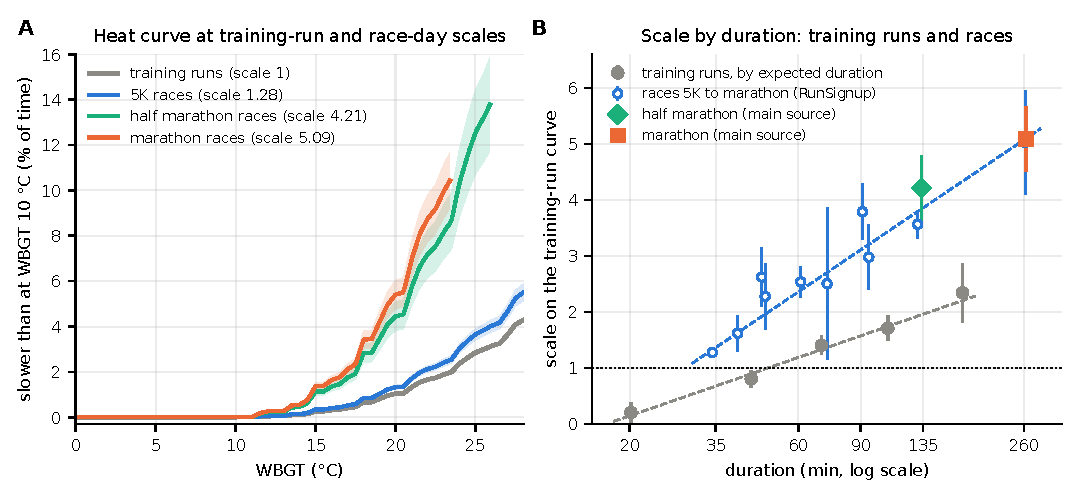
\includegraphics[width=\linewidth]{fig1_dose_response.pdf}
\caption{Training-run dose--response and race-day scale. \textbf{A}, the training-run heat curve \cW, the median runner's pace relative to WBGT 10\degC{} in counterfactual WBGT sweeps of the trained transformer (grey; zero at and below 10\degC), and the same curve multiplied by the race-day scales estimated from official results for the 5K (blue), the half marathon (green) and the marathon (orange); shaded bands are 95\% CI of the scale, and half-marathon and marathon curves are drawn up to the hottest edition in each set. \textbf{B}, within-runner scale on \cW{} for training runs in five bands of expected duration (grey; points at the band median; 95\% CI clustered by runner and by date and country; \nLtThirty, \nThirtySixty, \nSixtyNinety, \nNinetyOneFifty{} and \nGtOneFifty{} runs), race-day scales of ten distances from 5\,km to the marathon in the short-race source (open blue; course-clustered 95\% CI), and the half-marathon and marathon scales from the main official-results source (filled), placed at the median edition finish time. Dashed lines: fits on log duration across the training bands and across the ten race distances; dotted line: scale 1.}
\label{fig:dose}
\end{figure}

\begin{figure}[p]
\centering
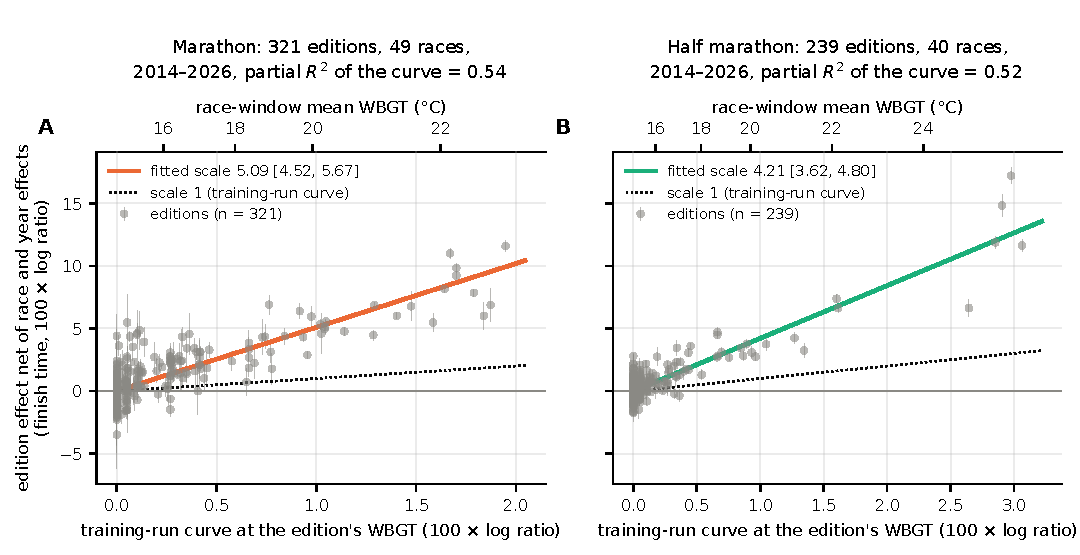
\includegraphics[width=\linewidth]{fig2_raceday_scale.pdf}
\caption{Within-person edition effects against the training-run curve at each edition's race-window WBGT. \textbf{A}, marathon, \nEdMar{} editions of \nRacesMar{} races; \textbf{B}, half marathon, \nEdHalf{} editions of \nRacesHalf{} races; 2014 to 2026 without 2020. Each point is an edition effect net of course and calendar-year fixed effects ($100 \times$ log ratio of finish time) with a 95\% CI from person-clustered standard errors. Solid line: fitted race-day scale (weighted least squares, weights $1/\mathrm{SE}^2$); dotted line: scale 1. The top axis gives the race-window mean WBGT corresponding to each curve value. Race-window WBGT is the mean from the first mass start to that start plus the edition's median finish time, at the start line. Panel titles give the partial $R^2$ of the curve beyond the fixed effects.}
\label{fig:raceday}
\end{figure}

\begin{figure}[p]
\centering
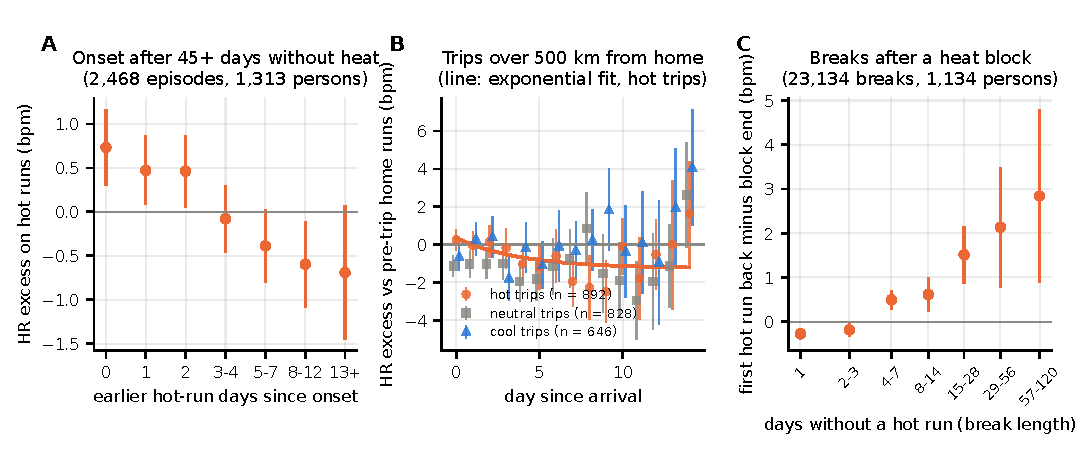
\includegraphics[width=\linewidth]{fig3_acclimation_kinetics.pdf}
\caption{Build and decay of heat acclimation in HR at matched load. The outcome is HR minus each runner's load model (pace, duration, climb), the start-hour effect and the population heat cost, relative to each design's baseline; heat is counted from WBGT 22\degC. \textbf{A}, onset: excess on hot runs by the number of earlier hot-run days after a first hot run that followed 45 or more days without one (episode fixed effects, days-since-onset trend, control for a hot run the day before; \kinOnsetEpisodes{} episodes). \textbf{B}, trips more than 500\,km from home: excess on away runs relative to home runs in the 45 days before the trip, by day since arrival, for hot ($\geq$5\degC{} warmer than home), neutral (within 2\degC) and cool ($\geq$5\degC{} cooler) trips; line, exponential fit to hot trips. \textbf{C}, breaks after a block of at least four hot-run days in 14: excess on the first hot run back minus the block's last week, by break length (\kinBreaks{} breaks). Means or coefficients with 95\% CI (person-clustered in A and C).}
\label{fig:kinetics}
\end{figure}

\begin{figure}[p]
\centering
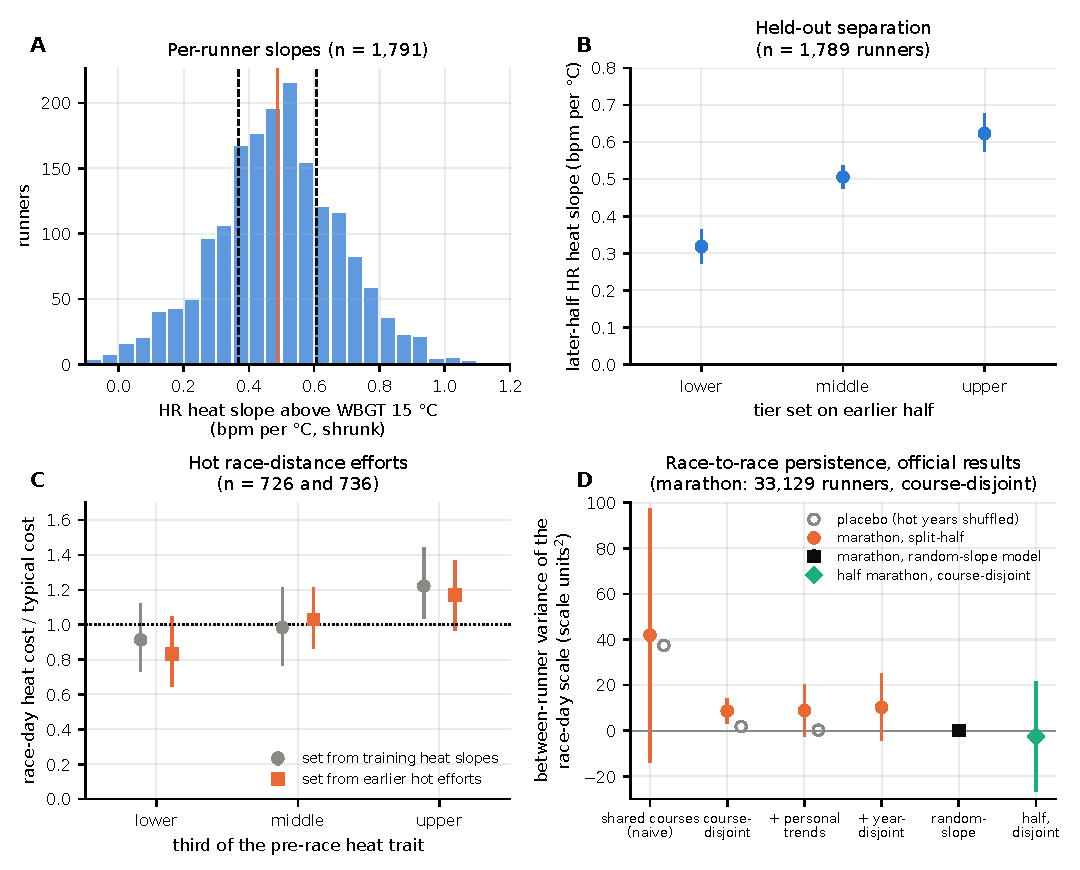
\includegraphics[width=\linewidth]{fig4_between_runner.pdf}
\caption{Between-runner differences in heat sensitivity in training and on race day. \textbf{A}, empirical-Bayes-shrunk HR heat slopes above WBGT 15\degC{} (\nSlopePersons{} runners); orange line, mean of the person slopes (\muPersons{} \bpmC); dashed lines, cut-points of three equal-probability tiers of the estimated true-slope distribution (\tierCuts{} \bpmC). \textbf{B}, later-half HR heat slope (mean and 95\% CI) by tier formed on the earlier half of each runner's history (\nTierRunners{} runners). \textbf{C}, race-day heat cost of hot race-distance efforts (WBGT 18\degC{} or above) by runners with at least one earlier hot effort, as a multiple of the population-typical cost after removing the runner's personal miss estimated from earlier data, by thirds of the training-derived heat trait (grey, \nTrainThirds{} efforts) or of the heat trait estimated from earlier race-distance efforts in the placement model (orange, \nEarlierThirds{} efforts); thirds use only data dated before each effort; 95\% CI from resampling runners; dotted line, typical cost. \textbf{D}, between-runner variance of the race-day scale in official results, estimated as the covariance of each runner's heat slopes from two halves of their races (95\% CI, delete-one-course jackknife): marathon halves sharing courses (naive), sharing no course, with personal trends, and sharing no calendar year; hollow markers, placebo with hot years shuffled within course; square, random-slope model on all repeat marathoners (upper bound shown); diamond, half marathon with halves sharing no course.}
\label{fig:between}
\end{figure}

\end{document}
